% documentclass options:
\documentclass[11pt,
  a4paper,
  parskip=half, % This is some extra vertical space between paragraphs, the suggestion is 2cm which is really ugly, so we use what koma script gives us
  % you can also set it to full for even more space. But there is a bad tex style decision: parskip also changes the spacing between listitems such as
  % enumerate and itemize. For this purpose we include the enumitem package and set itemsep=.5em, of course you can change this
  BCOR=10mm, % BCOR is binding correction
  english,
  % if you'd rather have a one sided thesis, add `oneside' to the documentclass
  oneside,
  % ngerman is needed for hyphenation if the thesis contains parts written in German, switch order with english if you write mainly in English.
  % Remember to change order in the babel package (below) as well.
  % Last language is the preferred one.
  ngerman]{scrbook}
\usepackage[english, ngerman]{babel} % If you write mainly in English change order to ngerman, english. Also change that in the documentclass options above.
% Include of titling must happen before \title etc.
% that's why it's not in setup.tex
\usepackage{titling}
\title{Analyse der Covid-19-Daten der deutschen Landkreise}
\author{Leander Marius Bürkin}

% Change to your first examiner
% The ~ enables non sentence spacing after a period
\newcommand{\firstexaminer}{Dr.~Andreas Greiner}
% Change to your second examiner, some undergraduate studies don't have a second examiner
% in this case just comment out the following line
\newcommand{\secondexaminer}{Prof.~Dr.~Moritz Mathias Diehl}
% Change to your adivers
\newcommand{\advisers}{Dr.~Andreas Greiner}

% include all packages and define commands in setup.tex

%------------------------------------------------------------------------------
%       package includes
%------------------------------------------------------------------------------
    % font encoding is set up for pdflatex, for other environments see
    % http://tex.stackexchange.com/questions/44694/fontenc-vs-inputenc
    \usepackage[T1]{fontenc}  % 8-bit fonts, improves handling of hyphenations
    \usepackage[utf8]{inputenc}
    % provides `old' commands for table of contents. Eases the ability to switch
    % between book and scrbook
    \usepackage{scrhack}

    % ------------------- layout, default -------------------
    % adjust the style of float's captions, separated from text to improve readabilty
    \usepackage[labelfont=bf, labelsep=colon, format=hang, textfont=singlespacing]{caption}
    % With format = hang your caption will look like this:
    % Figure 1: Lorem ipsum dolor sit amet,
    %           consectetuer adipiscing elit.
    %           Ut purus elit, vestibulum
    % If you instead want
    % Figure 1: Lorem ipsum dolor sit amet,
    % consectetuer adipiscing elit. Ut purus
    % elit, vestibulum
    % change to format=plain
    \usepackage{chngcntr}  % continuous numbering of figures/tables over chapters
    \counterwithout{equation}{chapter}
    \counterwithout{figure}{chapter}
    \counterwithout{table}{chapter}

    % Uncomment the following line if you switch from scrbook to book
    % and comment the setkomafont line
    %\usepackage{titlesec}  % remove "Chapter" from the chapter title
    %\titleformat{\chapter}[hang]{\bfseries\huge}{\thechapter}{2pc}{\huge}
    \setkomafont{chapter}{\normalfont\bfseries\huge}

    \usepackage{setspace}  % Line spacing
    \onehalfspacing
    % \doublespacing  % uncomment for double spacing, e.g. for annotations in correction

    % ------------------- functional, default-------------------
    \usepackage[dvipsnames]{xcolor}  % more colors
    \usepackage{array}  % custom format per column in table - needed on the title page
    \usepackage{graphicx}  % include graphics
    \usepackage{subfig}  % divide figure, e.g. 1(a), 1(b)...
    \usepackage{amsmath}  % |
    \usepackage{amsthm}   % | math, bmatrix etc
    \usepackage{amsfonts} % |
    \usepackage{calc}  % calculate within LaTeX
    \usepackage[unicode=true,bookmarks=true,bookmarksnumbered=true,
                bookmarksopen=true,bookmarksopenlevel=1,breaklinks=false,
                pdfborder={0 0 0},backref=false,colorlinks=false]{hyperref}
    \usepackage{etoolbox} % if-else commands


    %==========================================
    % You might not need the following packages, I only included them as they
    % are needed for the example floats
    % ------------------- functional, custom -------------------
    \usepackage{algorithm2e,algpseudocode}
    \usepackage{bm}  % bold greek variables (boldmath)
    \usepackage{tikz}
    \usetikzlibrary{positioning}  % use: above left of, etc
    
    % Required for the ToDo list.
    \usepackage{ifthen}

    % Improves general appearance of the text
    \usepackage[protrusion=true,expansion=true, kerning]{microtype}
    \usepackage{enumitem}
    % Nicer font for pdf rendering.
    %\usepackage{lmodern}
    
    % For nicer looking tables.
    \usepackage{booktabs}

    % You don't need this, just for demonstration of a longer caption.
    \usepackage{lipsum}

%------------------------------------------------------------------------------
%       (re)new commands / settings
%------------------------------------------------------------------------------
    % ----------------- referencing ----------------
    \newcommand{\secref}[1]{Sektion~\ref{#1}}
    \newcommand{\chapref}[1]{Kapitel~\ref{#1}}
    \renewcommand{\eqref}[1]{Gleichung~(\ref{#1})}
    \newcommand{\figref}[1]{Abbildung~\ref{#1}}
    \newcommand{\tabref}[1]{Tabelle~\ref{#1}}

    % ------------------- colors -------------------
    \definecolor{darkgreen}{rgb}{0.0, 0.5, 0.0}
    % Colors of the Albert Ludwigs University as in
    % https://www.zuv.uni-freiburg.de/service/cd/cd-manual/farbwelt
    \definecolor{UniBlue}{RGB}{0, 74, 153}
    \definecolor{UniRed}{RGB}{193, 0, 42}
    \definecolor{UniGrey}{RGB}{154, 155, 156}


    % ------------------- layout -------------------
    % prevents floating objects from being placed ahead of their section
    \let\mySection\section\renewcommand{\section}{\suppressfloats[t]\mySection}
    \let\mySubSection\subsection\renewcommand{\subsection}{\suppressfloats[t]\mySubSection}



    % ------------------- math formatting commands -------------------
    % define vectors to be bold instead of using an arrow
    \renewcommand{\vec}[1]{\mathbf{#1}}
    \newcommand{\mat}[1]{\mathbf{#1}}
    % tag equation with name
    \newcommand{\eqname}[1]{\tag*{#1}}


    % ------------------- pdf settings -------------------
    % ADAPT THIS
    \hypersetup{pdftitle={\thetitle},
                pdfauthor={\theauthor},
                pdfsubject={Undergraduate thesis at the Albert Ludwig University of Freiburg},
                pdfkeywords={simulation, corona, covid19, model reconstruction, diffusion, spreading},
                pdfpagelayout=OneColumn, pdfnewwindow=true, pdfstartview=XYZ, plainpages=false}


    %==========================================
    % You might not need the following commands, I only included them as they
    % are needed for the example floats

    % ------------------- Tikz styles -------------------
    \tikzset{>=latex}  % arrow style


    % ------------------- algorithm ---------------------
    % Command to align comments in algorithm
    \newcommand{\alignedComment}[1]{\Comment{\parbox[t]{.35\linewidth}{#1}}}
    % define a foreach command in algorithms
    \algnewcommand\algorithmicforeach{\textbf{foreach}}
    \algdef{S}[FOR]{ForEach}[1]{\algorithmicforeach\ #1\ \algorithmicdo}

    % line spacing should be 1.5
    \renewcommand{\baselinestretch}{1.5}

    % set distance between items in a list, for more details see the
    % enumitem package: https://www.ctan.org/pkg/enumitem
    \setlist{itemsep=.5em}
    
    % use ra in your tables to increase the space between rows
    % 1.3 should be fine
    \newcommand{\ra}[1]{\renewcommand{\arraystretch}{#1}}

	% ToDo counters
	\usepackage{ifthen} %für whiledo-Schleife
	\newcounter{todos}
	\setcounter{todos}{0}
	\newcounter{extends}
	\setcounter{extends}{0}
	\newcounter{drafts}
	\setcounter{drafts}{0}

	% ------------------- marker commands -------------------
    % ToDo command
    \newcommand{\todo}[1]{\textbf{\textcolor{red}{(TODO: #1)}}\refstepcounter{todos}\label{todo \thetodos}}
	\newcommand{\extend}[1]{\textbf{\textcolor{darkgreen}{(EXTEND: #1)}}\refstepcounter{extends}\label{extend \theextends}}
	% Lighter color to note down quick drafts
	\newcommand{\draft}[1]{\textbf{\textcolor{NavyBlue}{(DRAFT: #1)}}\refstepcounter{drafts}\label{draft \thedrafts}}
	
	% microtype with lmodern, see https://tex.stackexchange.com/questions/75305/microtype-warning-with-lmodern-package-and-koma-script
	%\DeclareMicrotypeAlias{lmss}{cmr}
	
	\renewcommand{\listalgorithmcfname}{Algorithmenverzeichnis}
	\renewcommand{\algorithmcfname}{Algorithmus}
	
	
	
%  ------------------- my own packages -------------------

    
    % to add biber/biblatex handling the references
    \usepackage[backend=biber]{biblatex}
    \addbibresource{References/Refs_Grundlagen_und_Stand_der_Forschung.bib}
    \addbibresource{References/Refs_Motivation.bib}
    \addbibresource{References/Refs_Zitatseite.bib}
    \usepackage{csquotes}
    
    % to prevent underfull/overfull hbox
    \usepackage{parskip}

    % to pack content into multiple cells of a table
    \usepackage{multirow}

\begin{document}
    \pagestyle{empty} % no header and no page number
    % disable hyper links to remove warning "destination with same identifier"
    % this means within this section nothing can be referenced with a hyperlink
    \hypersetup{pageanchor=false}

    % enable/disable, depending on your chosen language
    \begin{titlepage}
\begin{center}
\ \\
\newcommand{\HorizontalLine}{\rule{\linewidth}{0.3mm}}
{\large Bachelorarbeit}\\[-0.5cm]
\HorizontalLine \\[0.4cm]
{ \huge \bfseries \thetitle }
\HorizontalLine \\[0.7cm]

{\huge \theauthor} \\[0.3cm]
\begin{tabular}[hc]{>{\large}l >{\Large}l}
  Gutachter: & \advisers \\[1cm]
\end{tabular}
\setlength{\fboxrule}{2pt}
\setlength{\fboxsep}{0pt}
\fbox{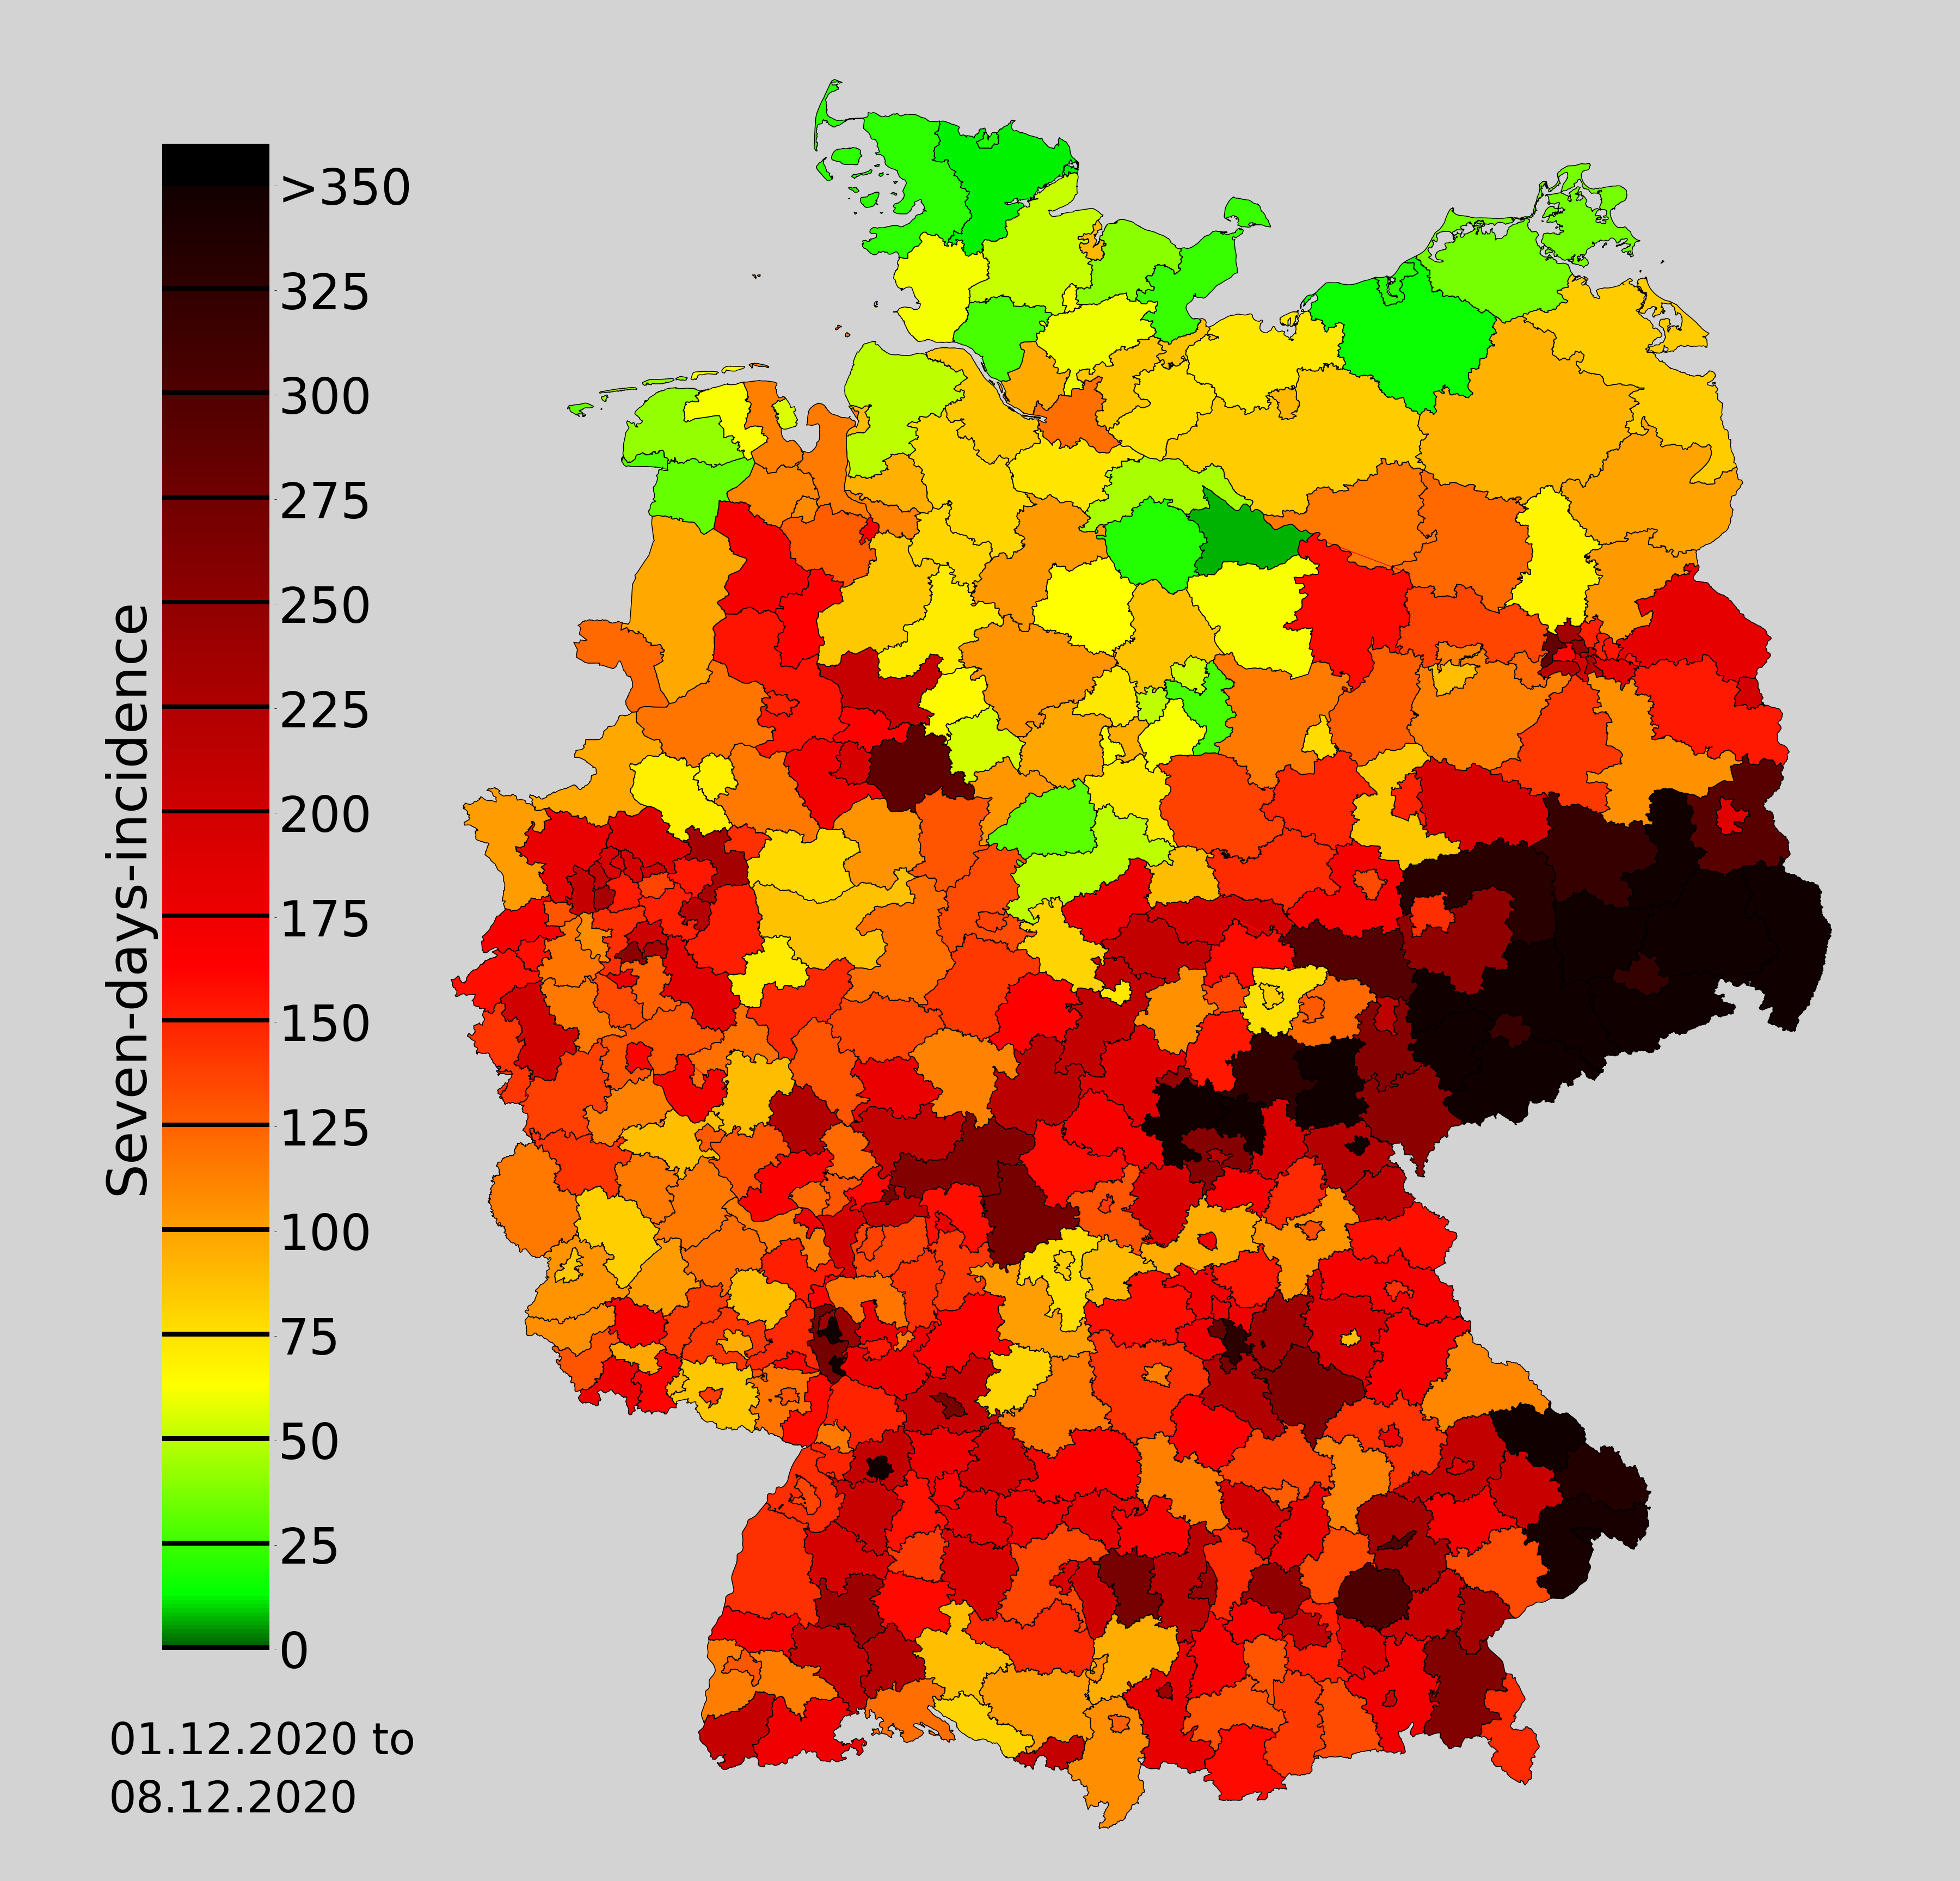
\includegraphics[width=0.6\textwidth]{figures/vor_dem_Inhaltsverzeichniss/282lightgrey.png}}
\\[1cm]
Lehrstuhl für Simulation\\[-0.25cm]
Institut für Mikrosystemtechnik - IMTEK\\[-0.25cm]
Albert-Ludwigs-Universität, Freiburg im Breisgau
\end{center}
\end{titlepage}

\thispagestyle{empty}
\ \vfill \ \\
\
\textbf{Bearbeitungszeit}           \smallskip{} \\
02.\,04.\,2021 -- 08.\,08.\,2021    \bigskip{} \\
\
\textbf{Gutachter}                  \smallskip{} \\
\firstexaminer                      \bigskip{} \\
\
% If there is a second examiner include it
\textbf{Zweitgutachter}             \smallskip{} \\
\secondexaminer                     \bigskip{} \\
\
\textbf{Betreuer}                   \smallskip{} \\
\advisers

    \pagestyle{plain} % remove chapter name from top, page number at the bottom
    % use \pagestyle{headings} for having the chapter on top of the pages
    % if you wang a more fancy header use \usepackage[automark,headsepline]{scrlayer-scrpage}
    % and read about it in the KOMA script documentation, https://www.ctan.org/pkg/koma-script
    \frontmatter  % roman page numbers
    \chapter*{Erklärung}
Hiermit erkläre ich, dass ich diese Abschlussarbeit selbständig verfasst habe, keine anderen als die angegebenen Quellen/Hilfsmittel verwendet habe und alle Stellen, die wörtlich oder sinngemäß aus veröffentlichten Schriften entnommen wurden, als solche kenntlich gemacht habe. Darüber hinaus erkläre ich, dass diese Abschlussarbeit nicht, auch nicht auszugsweise, bereits für eine andere Prüfung angefertigt wurde.
\\[3\normalbaselineskip]
\begin{tabular}{p{\textwidth/2} l}
  \rule{\textwidth/3}{0.4pt}   &   \rule{\textwidth/3}{0.4pt} \\
  Ort, Datum                  &   Unterschrift
\end{tabular}

    \chapter*{Abstract}
2020 and 2021 have been marked by COVID-19 and the ensuing uncertainty:
How does the virus spread? Does the virus spread from the cities to rural areas? Can the counties whose case numbers skyrocketed earlier be categorized in any way? Or more generally: is the spread of the virus SARS-CoV-2 correlated with certain characteristics of a given area?

An attempt to answer these questions and to summarize the given data is described in this thesis. The project uses data provided by the Robert Koch Institute (RKI).

On the basis of the processed data, an SIR model for Germany is created and several correlation analyses of data regarding COVID-19 from various administrative districts are carried out.
Finally, the results are plotted and interpreted in order to make the elusive COVID-19 infection patterns accessible.

\chapter*{Kurzfassung}
Die Jahre 2020 und 2021 waren von der COVID-19-Pandemie und der einhergehenden Unsicherheit geprägt:
Wie verbreitet sich das Virus? Breitet sich das Virus von den Städten ausgehend in die ländlichen Gebiete aus? Lassen sich die Stadt- und Landkreise, deren Fallzahlen früher in die Höhe schießen, kategorisieren? Oder ganz allgemein: Korreliert die Ausbreitung von SARS-CoV-2 mit bestimmten Eigenschaften von Gebieten?

Ein Versuch, diese Fragen zu beantworten und die gegebenen Daten zusammenzufassen, Gegenstand dieser Arbeit beschrieben. Hierbei wird mit Daten gearbeitet, welche das Robert Koch-Institut (RKI) zur Verfügung stellt.

Auf Basis der aufgearbeiteten Daten wird ein SIR-Modell für Deutschland erstellt und mehrere Korrelationsanalysen von den Daten der kreisfreien Städte, Landkreise und Regierungsbezirke zu der COVID-19-Pandemie durchgeführt.
Zuletzt werden graphische Darstellungen der Ergebnisse erstellt und interpretiert, um das schwer greifbare Infektionsgeschehen des Virus SARS-CoV-2 zugänglich zu machen.
\newpage
    \vspace*{15pt}
\begin{center}
    \huge{\textbf{
    \textit{Those who cannot remember the past\\ are condemned to repeat it.}}}
    \large{- George Santayana \autocite{history-quoteSantayana}}
\end{center}
\vspace*{65pt}
\begin{figure}[h]
    \centering
    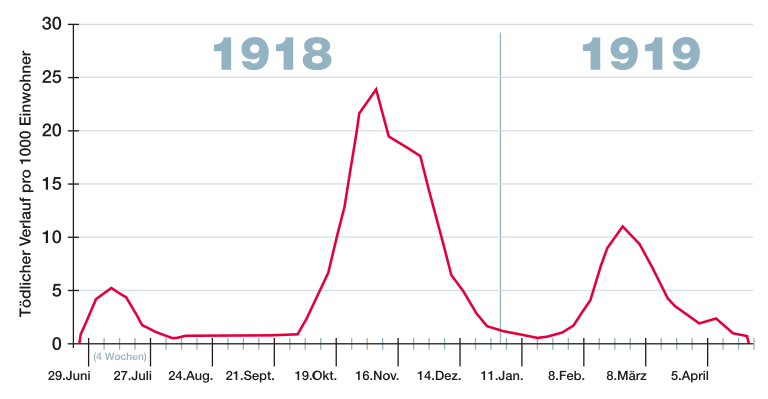
\includegraphics[width=0.71\textwidth]{figures/vor_dem_Inhaltsverzeichniss/Spanische_Grippe_1918_1919_GB.svg.png}
    \caption{Die drei Wellen der \glqq{}Spanischen Grippe\grqq{} in Großbritannien, wöchentliche kombinierte Grippe- und Lungenentzündungssterblichkeit von Juni 1918 bis Mai 1919. \autocite{spanischflu}}
    \label{fig:spanishflu}
\end{figure}

\begin{figure}[h]
    \centering
    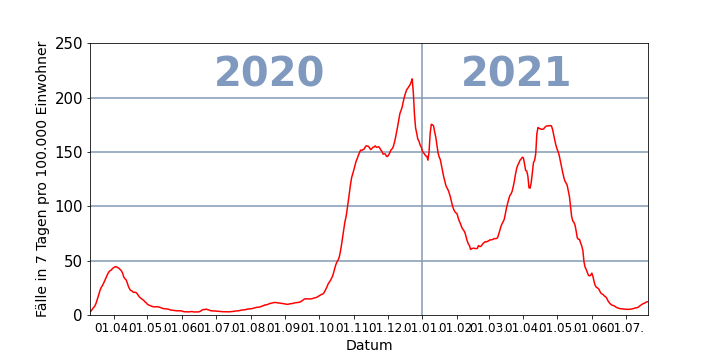
\includegraphics[width=0.76\textwidth]{figures/vor_dem_Inhaltsverzeichniss/Inzidenz_Deutschland.png}
    \caption{Die drei Wellen der COVID-19-Pandemie in Deutschland, dargestellt durch die sieben Tage Inzidenz jeden Tages über den Zeitraum vom 01.03.2020 bis 05.06.2021.}
    \label{fig:germany_incidence}
\end{figure}
    \tableofcontents
    \listoffigures
    %\listoftables
    %\listofalgorithms
    \hypersetup{pageanchor=true}  % re-enable hyperlinking

    \mainmatter  % Arabic page numbers
    \chapter{Motivation}\label{chap:Motivation}
Viele große Zivilisationen hatten bereits mit Pandemien ähnlich zur aktuellen COVID-19 Pandemie zu kämpfen.\\
Schon aus dem Alten Rom haben wir Zeugnisse der Antoninischen Pest im zweiten Jahrhundert nach Christus: Vermutlich ein Pocken Ausbruch, dessen 7-10 Millionen Tote das Römische Reich destabilisierten (\autocite{RomPest}, S. 255).
Im Mittelalter kamen 200 Millionen Menschen durch die Pest um \autocite{PestMittelalter}.
Die Armeen des ersten Weltkriegs wurden ebenfalls durch die Spanische Grippe geschwächt: Sie forderte circa 100 Millionen Opfer weltweit \autocite{SpanischeGrippe}.

Doch nicht nur in den dicht besiedelten Gebieten des Mittelmeerraums und des Nahen Ostens sorgten Pandemien für Instabilität: Sie sind seit jeher ein weltweites Problem und können durch Reisen ausgleöst oder stark verstärkt werden.\\
Nach 1707 starben innerhalb von zwei Jahren circa 18.000 der 50.000 Einwohner Islands an Pocken (\autocite{americaPandemics}, Seite 325 Zeile 20ff). Vieles spricht für einen ähnlich vernichtenden Pockenausbruch bei den Azteken, den Inka und den andere Völkern der Neuen Welt \autocite{americaPandemics}.

Über diese vergangenen Pandemien wissen wir recht wenig, da sie beispielsweise durch den Zorn Gottes erklärt wurden(\autocite{americaPandemics}, Seite 324 Zeile 7) oder die genannten Zahlen eher die Gefühle der Zeitzeugen widerspiegeln als statistische Daten zu liefern (\autocite{americaPandemics}, Seite 324 Zeile 20ffff). Mit dem heutigen Stand der Datenerfassung und -übermittlung lässt sich die COVID-19 Pandemie sehr viel einfacher untersuchen als ihre Vorgänger.

um derartige Todeswellen zu vermeiden und einer Zivilisation Stabilität zu bieten, ist es wichtig, diese einschneidenden Ereignisse mit verschiedensten Ansätzen zu untersuchen. 

Die meisten von uns haben genau diese Zahlen des Robert-Koch-Instituts oder der Weltgesundheitsorganisation beobachtet und versucht zu verstehen, wie man sich morgen zu Verhalten hat. Viele Hypothesen wurden aufgestellt und jede*r musste sich auf einmal mit Epidemiologie beschäftigen, wobei wir meist nur ein Puzzleteil vor Augen hatten.

Trotz immenser Bemühungen brachte die aktuelle COVID-19 Pandemie unser Gesundheitssystem an seine Grenzen: Kleinere Krankenhäuser wurden schnell überwältigt, wenn der Bedarf an Beatmungsgeräten größer wurde als ihre Kapazitäten.

Daher soll diese Arbeit das gesellschaftliche Verständniss für zukünftigen Pandemien schärfen, damit die Ausbreitung zukünfitger Erreger verlangsamt wird und ein Kollaps des Gesundheitssystems oder gar der gesamten Zivilisation verhindert werden kann.

    \chapter{Grundlagen}\label{chap:Grundlagen}

\section{Mittelwert}\label{sec:Grundlagen:Mittelwert}
Der Mittelwert, das Mittel oder auch der Durchschnitt entspricht nach \autoref{eq:Mittelwert} der Summe der einzelnen Werte $x_1$, $x_2$, $x_3$ ... $x_n$ geteilt durch ihre Anzahl $n$.
\begin{equation}\label{eq:Mittelwert}
    \bar x = \frac{1}{n}\sum_{i=1}^n x_i
\end{equation}

\section{Susceptible-Infectious-Removed-Modell}\label{sec:Grundlagen:SIR}
Ein Weg zur Beschreibung der Pandemie bietet das \glqq{}Susceptible-Infectious-Removed-Modell\grqq{} (SIR-Modell) \autocite{SIR}. Dieses Modell teilt die Mitglieder einer Menschengruppe in eine der drei folgenden Kategorien ein und ermöglicht es, die zeitliche Entwicklung einer Pandemie übersichtlich darzustellen:
\begin{itemize}
    \item \glqq{}Susceptible\grqq{}: Menschen, welche angesteckt werden können.
    \item \glqq{}Infectious\grqq{}: Infizierte Menschen, welche weitere Menschen anstecken können. Werden auch als \glqq{}die aktiven Fälle\grqq{} bezeichnet.
    \item \glqq{}Removed\grqq{}: Menschen, welche in die Kategorie \glqq{}Infectious\grqq{} fielen, nun keine weiteren Menschen mehr anstecken können und aus dem Infektionsgeschehen entfernt wurden,
    in diesem Fall Genesene und Verstorbene. 
\end{itemize}
In dem hier verwendeten SIR-Modell wird weder die Geburten- noch die Sterberate beachtet, die angenommen Bevölkerung bleibt durchgehend konstant.

Zudem wird angenommen, das jedes Individuum nur einmal infiziert werden kann und die Infektion die einzige Möglichkeit darstellt, von der Kategorie \glqq{}Susceptible\grqq{} in die Kategorie \glqq{}Removed\grqq{} zu wechseln.
Somit fällt die Zahl der Menschen in der Kategorie \glqq{}Susceptible\grqq{} monoton und die Zahl der Menschen in der Kategorie \glqq{}Removed\grqq{} steigt monoton an.\autocite{SIR}

\section{Bevölkerungsdichte}
Die Bevölkerungsdichte eines Gebietes $\rho_{Gebiet}$ wird berechnet, indem die Anzahl der Einwohner im Gebiet $n_{Einwohner\ Gebiet}$ durch die Fläche des Gebiets $A_{Gebiet}$ geteilt wird:
\begin{equation}\label{eq:Bevölkerungsdichte}
    \rho_{Gebiet} = \frac{n_{Einwohner\  Gebiet}}{A_{Gebiet}}
\end{equation}
\section{7-Tages Inzidenz}\label{sec:Grundlagen:7-Tages Inzidenz}
Die 7-Tages Inzidenz ist laut RKI als die \glqq{}Anzahl der innerhalb der letzten 7 Tage neu gemeldeten Fälle pro 100.000 Einwohner\grqq{} definiert \autocite{7-TageInzidenz}.

Um die 7-Tages Inzidenz $i_d$ für den Tag $d$ zu berechnen, wird von der akkumulierten Zahl der Fälle  am gewählten Tag $f_d$ die akkumulierte Zahl der Fälle sieben Tage zuvor $f_{d-7}$ abgezogen, dies ergibt die neu hinzugekommenen Fälle innerhalb von sieben Tagen.

Schlussendlich wird diese Zahl durch die Anzahl der Bewohner des Gebiets $p_{Gebiet}$ geteilt und mit 100 000 multipliziert. Dies ergibt \autoref{eq:7-Tages_Inzidenz}.
\begin{equation}\label{eq:7-Tages_Inzidenz}
    i_t= \frac{f_d-f_{d-7}}{p_{Gebiet}}\cdot 100.000
\end{equation}

Die 7-Tages Inzidenz bietet sich im Vergleich zur täglichen Fallzahl aus mehreren Gründen als Kennzahl für die Verbreitung eines Virus in einem Gebiet an:

Wie in \autoref{fig:neue_Fälle_pro_Wochentag_Deutschland} klar zu sehen, werden an Wochenenden im Schnitt deutlich weniger neue Fälle registriert als an den anderen Wochentagen.
Daher werden immer sieben Tage in der 7-Tages Inzidenz zusammengefasst.
\begin{figure}[H]
    \centering
    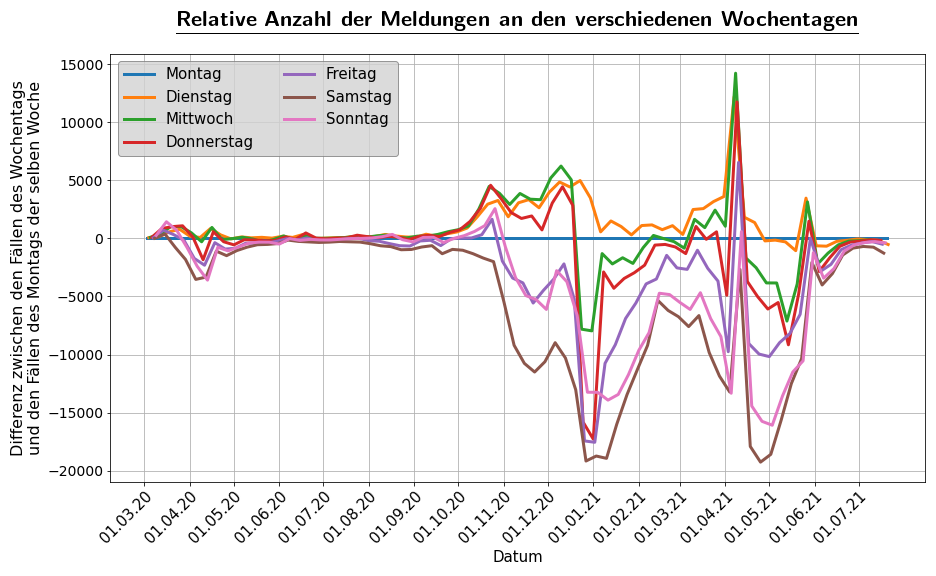
\includegraphics[width=0.95\textwidth]{figures/Grundlagen/neue_Fälle_pro_Wochentag_Deutschland.png}
    \caption{In Deutschland neu gemeldete COVID-19 Fälle am jeweiligen Wochentag im Vergleich zu den am Montag der selben Woche gemeldeten Fälle.}
    \label{fig:neue_Fälle_pro_Wochentag_Deutschland}
\end{figure}
Da die Bevölkerung der deutschen Landkreise und Regierungsbezirke nicht identisch ist, wird jeweils durch die Bevölkerungszahl geteilt, um die einzelnen Gebiete miteinander vergleichen zu können.

Aufgrund der ansonsten sehr kleinen Zahlen, bietet es sich zudem an, das Ergebnis mit 100.000 zu multiplizieren.

Dies sind die drei Begründungen für die drei Schritte in der Berechnung der 7-Tages Inzidenz nach \autoref{eq:7-Tages_Inzidenz}.


\section{Korrelationsanalyse mithilfe einer Faltung}\label{sec:BeschreibungKorrelationsanalyse}

\subsection{Berechnung der Korrelationswerte}\label{sec:Grundlagen:BerechnungderKorrelationwertes}
Um festzustellen, ob die 7-Tages Inzidenzen einiger Landkreise im Vergleich zu anderen Landkreisen eher voraus- oder nacheilen, wird die Korrelationsfunktion verwendet \autocite{Korrelation}.

Bei diskreten Werten, aufgeteilt in zwei Zeitserien $X$ und $Y$, wie in diesem Fall, basiert die Korrelationsanalyse auf einer diskreten Faltung:
Für eine zeitliche Verschiebung $\tau$ wird mit jedem Wert $x_i$ zum jeweiligen Zeitpunkt $t_i$ aus der ersten Zeitserie mit dem zugehörigen Wert $y_i$ aus der zweiten Zeitserie ein Produkt gebildet. Der zugehörige Wert aus der zweiten Zeitserie entspricht hierbei dem Zeitpunkt $t$ des Wertes der ersten Zeitserie plus die gewählte Verschiebung $\tau$. Sollte dieser zweite Wert nicht existieren, wird kein Produkt gebildet.

Für jede zeitliche Verschiebung $\tau$, für die mindestens ein Produkt gebildet wird, werden alle möglichen Produkte aufsummiert.

Somit ergibt sich \autoref{eq:Korrelation}, mit $n := $ Länge von $X$ und wenn $y_{i+\tau} \not\in Y$, dann $y_{i+\tau} := 0$:
\begin{equation}\label{eq:Korrelation}
    c(\tau) = \sum_{i=1}^n x_i\cdot y_{i+\tau}
\end{equation}


Bildlich gesprochen wird die zweite Zeitserie an der ersten Zeitserie vorbeigeschoben, beginnend an dem Punkt, an dem ausschließlich das erste Element der ersten Zeitserie mit dem letzten Element der zweiten Zeitserie multipliziert wird. Dies ist beispielhaft mit den Folgen $[1,2,3,2]$ und $[5,7,5,1]$ in \autoref{fig:Korrelation Beispiel} dargestellt.

\begin{figure}[H]
    \centering
    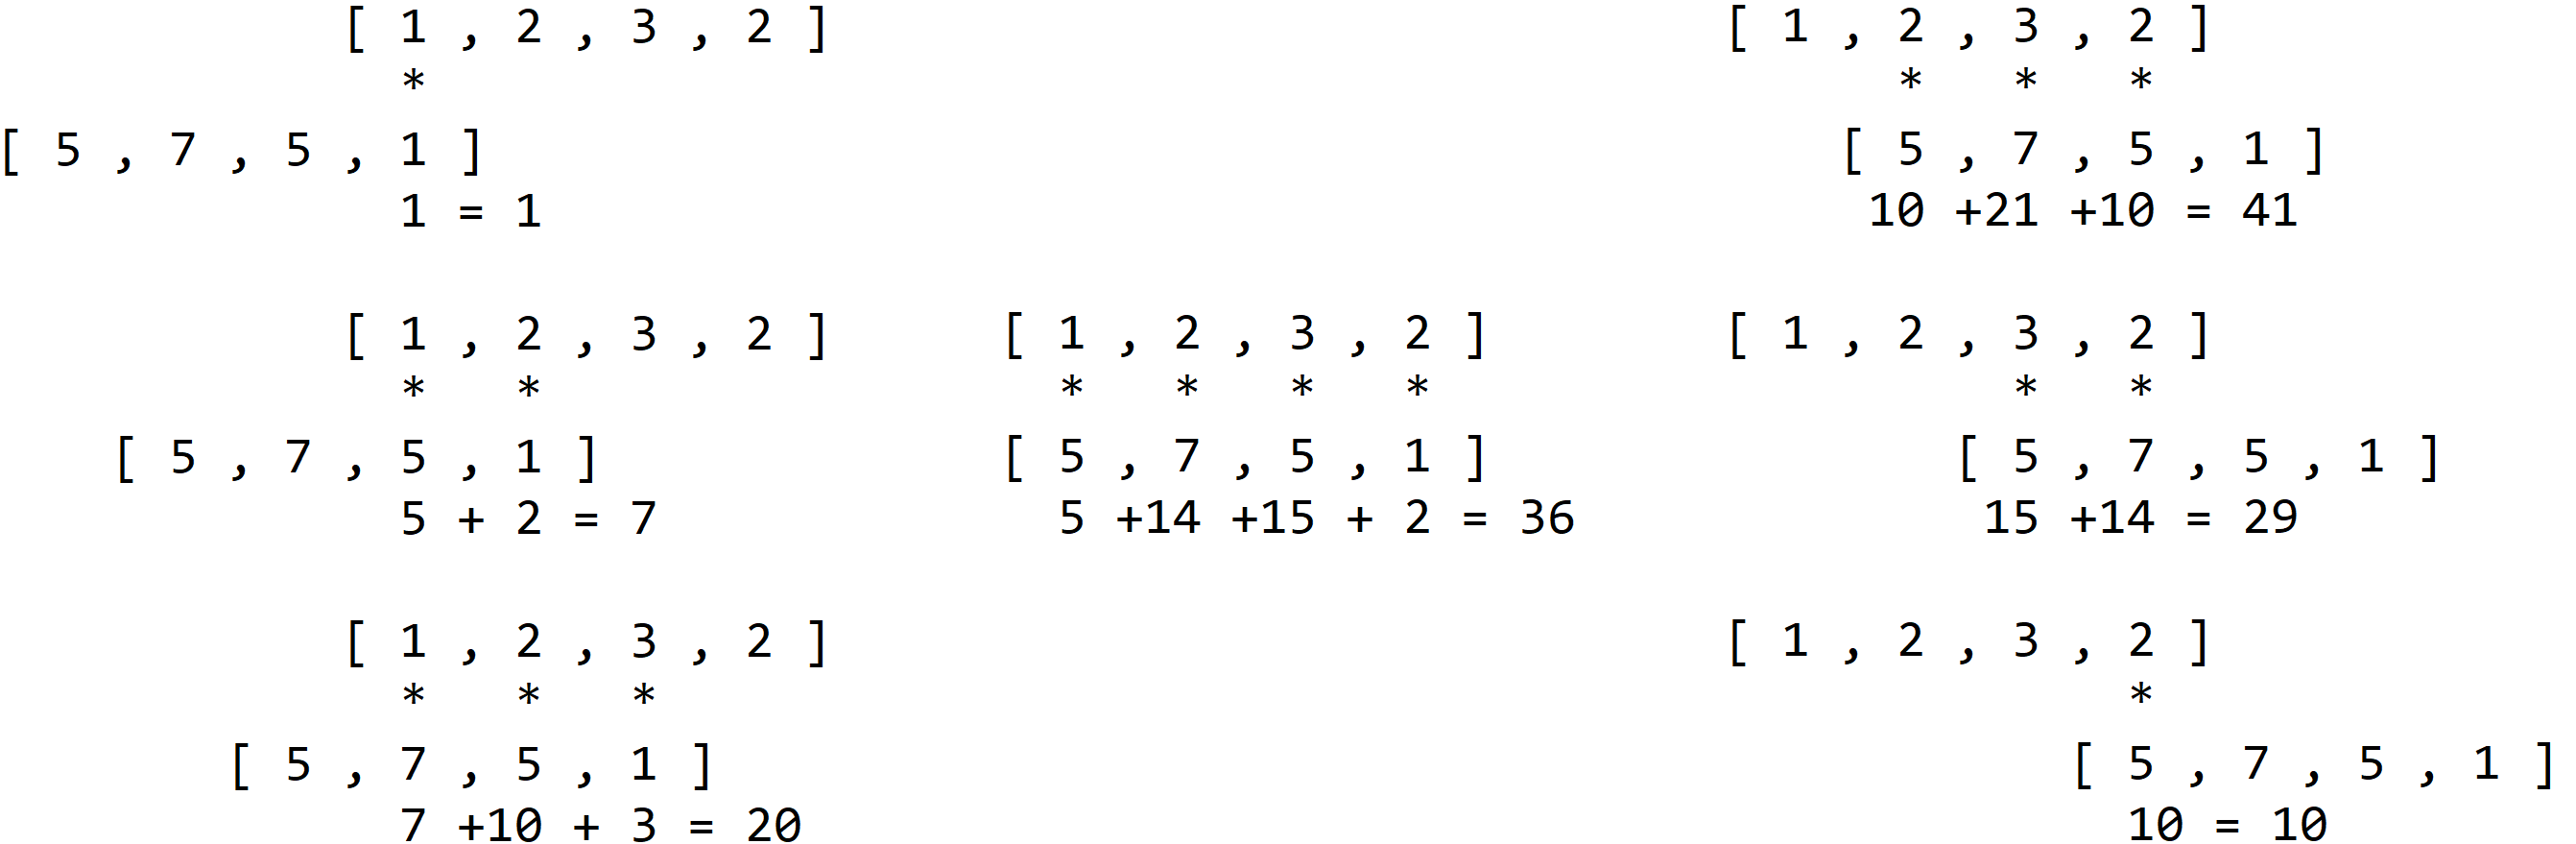
\includegraphics[width=\textwidth]{figures/Grundlagen/Korrelation.png}
    \caption{Beispielhafte Darstellung einer Faltung anhand der Folgen $[1,2,3,2]$ und $[5,7,5,1]$. Auf der linken Seite sind von oben nach unten hinter dem Gleichheitszeichen die Korrelationswerte für die negativen Verschiebungen $\tau=-3$, $\tau=-2$ und $\tau=-1$ eingetragen. Entsprechend ist der Korrelationswert für die Verschiebung $\tau=0$ in der Mitte und die Korrelationswerte für die positiven Verschiebungen $\tau=1$, $\tau=2$ und $\tau=3$ auf der rechten Seite zu finden.}
    \label{fig:Korrelation Beispiel}
\end{figure}

Da bei einer Korrelationsanalyse nach \autoref{eq:Korrelation} Summen aus mehr Produkten übergewichtet werden und Zeitserien mit größeren Werten größere Korrelationswerte erzeugen, müssen die Korrelationswerte noch skaliert werden.

Um zum einen die unterschiedliche Anzahl der Produkte auszugleichen, werden die Summen durch die Anzahl ihrer Summanden geteilt, wie in \autoref{eq:skalierte_Korrelation_geteilt_durch_Produkte} gezeigt. Ohne diese Gewichtung würden zwei Zeitserien mit konstanten Werten größer null bei einer Verschiebung $\tau=0$ die größte Korrelation aufweisen und die Korrelation bei betragsmäßig größeren Verschiebungen abnehmen, was nicht gewünscht ist.

Da jede Zeitserie die gleiche Länge $n$ hat, erhält man die Anzahl der Summanden indem man
den Betrag der Verschiebung $\vert\tau\vert$
von der Länge der Zeitserie $n$ abzieht:

\begin{equation}\label{eq:skalierte_Korrelation_geteilt_durch_Produkte}
    c(\tau) =\frac{1}{n-\vert\tau\vert} \sum_{i=1}^n x_i\cdot y_{i+\tau}
\end{equation}

Um zum anderen die tendenziell größeren Werte mancher Zeitserien auszugleichen, werden die Werte aller Zeitserien mithilfe des sogenannten \glqq{}Autokorrelationswerts für die Verschiebung $\tau=0$ \grqq{} gewichtet: Er beschreibt den Wert der Korrelation einer Zeitserie mit sich selbst bei keiner zeitlichen Verschiebung. Wie in \autoref{eq:skalierte_Korrelation} zu sehen, werden die Werte einer Zeitserie gewichtet, indem sie durch die Wurzel des Autokorrelationswerts für die Verschiebung $\tau=0$ dieser Zeitserie geteilt werden.

\begin{equation}\label{eq:skalierte_Korrelation}
    c(\tau) =
    \frac{1}{n-\vert\tau\vert}
    \sum_{i=1}^n
    \frac{x_i}{\sqrt{\frac{1}{n}\sum_{i=1}^n x_i^2}}
    \cdot
    \frac{y_{i+\tau}}{\sqrt{\frac{1}{n}\sum_{i=1}^n y_i^2}}
    =
    \frac{n}{n-\vert\tau\vert}
    \frac{\sum_{i=1}^n x_i \cdot y_{i+\tau}}
    {\sqrt{\sum_{i=1}^n x_i^2}
    \sqrt{\sum_{i=1}^n y_i^2}}
\end{equation}


Zudem wird von jedem Wert der Zeitserie $x_i$ der Mittelwert $\overline x = \frac{1}{n}\sum_{i=1}^n x_i$ abgezogen, dadurch lassen sich Antikorrelationen feststellen: Wenn beispielsweise die Anzahl der COVID-19 Infektionen eines Landkreises zu einem Zeitpunkt überdurchschnittlich wächst, also die 7-Tages-Inzidenz minus dem Mittelwert der 7-Tages-Inzidenzen positiv ist, und das andere Edukt aus der anderen Zeitserie negativ ist, also in dem anderen Landkreis die Anzahl der COVID-19 Infektionen unterdurchschnittlich wächst, ergibt sich ein negatives Produkt, da sich die Situation in dem einen Landkreis  schneller als üblich verschlechtert, während sich die Situation im anderen Landkreis verbessert oder langsamer als üblich verschlechtert.

Ergibt die Summe aus all den Produkten einer Korrelation eine negative Zahl, scheint die 7-Tages Inzidenz des einen Landkreises zu fallen oder langsam zu steigen, während die 7-Tages Inzidenz des anderen Landkreises steigt oder langsam fällt, dies wird hier Antikorrelation genannt.

Mit allen Ergänzungen berechnet sich die Korrelation $c(\tau)$ zwischen der Zeitserie $X:|X|=n$ mit den Werten $x_i\in X$ und der Zeitserie $Y:|Y|=n$ mit den Werten $y_i \in Y$ und einer Verschiebung $\tau$ relativ zu $X$ mithilfe der Mittelwerte der Zeitserien $\overline x,\ \overline y$ wie in \autoref{eq:komplette_skalierte_Korrelation} beschrieben.
\begin{equation}\label{eq:komplette_skalierte_Korrelation}
    c(\tau) =\frac{n}{n-\vert\tau\vert}
    \frac{\sum_{i=1}^n (x_i-\overline x)\cdot (y_{i+\tau}-\overline y)}{\sqrt{\sum_{i=1}^n (x_i-\overline x)^2}\sqrt{\sum_{i=1}^n (y_i-\overline y)^2}}
\end{equation}

\subsection{Korrelation zwischen zwei Gebieten am Beispiel von Flensburg und Kiel}
Um die verwendete Terminologie und die hergeleiteten Gleichungen anhand eines Beispiels näher zu bringen, werden in diesem Abschnitt die einzelnen Schritten einer Korrelationsanalyse ausgeführt. Als Beispiel dient hierfür die Korrelation zwischen den 7-Tages Inzidenzen der Stadtkreise Flensburg und Kiel. Die 7-Tages Inzidenzen sind in \autoref{fig:Inzidenz_Flensburg} und \autoref{fig:Inzidenz_Kiel} abgebildet, jeweils einmal im Original und einmal um den Mittelwert der 7-Tages Inzidenz in x-Richtung nach unten verschoben.

\begin{figure}[H]
    \centering
    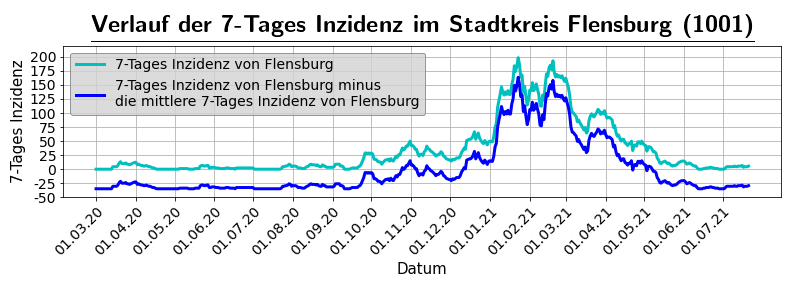
\includegraphics[width=0.95\textwidth]{figures/Grundlagen/Inzidenz_Flensburg.png}
    \caption{Der Verlauf der 7-Tages Inzidenz des Stadtkreises Flensburg (Gemeindeschlüssel 1001).
    In Hellblau ist der originale Verlauf der 7-Tages Inzidenz dargestellt. Der Verlauf der 7-Tages Inzidenzen, von denen der Mittelwert der 7-Tages Inzidenzen von Flensburg abgezogen wurde, ist blau dargestellt.}
    \label{fig:Inzidenz_Flensburg}
\end{figure}
\begin{figure}[H]
    \centering
    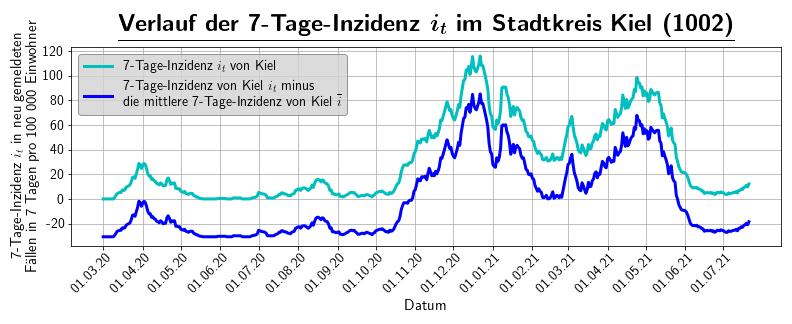
\includegraphics[width=0.95\textwidth]{figures/Grundlagen/Inzidenz_Kiel.png}
    \caption{Der Verlauf der 7-Tages Inzidenz des Stadtkreises Kiel (Gemeindeschlüssel 1002).
    In Hellblau sind ist der originale Verlauf der 7-Tages Inzidenz dargestellt. Der Verlauf der 7-Tages Inzidenzen, von denen der Mittelwert der 7-Tages Inzidenzen von Kiel abgezogen wurde, ist blau dargestellt.}
    \label{fig:Inzidenz_Kiel}
\end{figure}
In \autoref{fig:correlation_Flensburg_Kiel} ist die diskrete Faltung abgebildet, wie sie der Korrelationsanalyse zugrunde liegt und in \autoref{eq:Korrelation} definiert ist.
\begin{figure}[H]
    \centering
    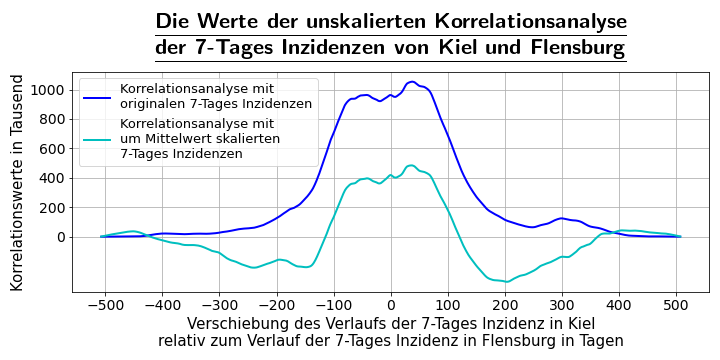
\includegraphics[width=0.95\textwidth]{figures/Grundlagen/correlation_Flensburg_Kiel.png}
    \caption{Ergebnis der diskreten Faltung der 7-Tages Inzidenzen der Stadtkreise Kiel und Flensburg.
    In Hellblau ist das Ergebnis der Faltung mit den originalen 7-Tages Inzidenzen dargestellt. Das Ergebnis der Faltung mit den 7-Tages Inzidenzen, von denen der Mittelwert der 7-Tages Inzidenzen des jeweiligen Landkreises abgezogen wurde, ist blau dargestellt.}
    \label{fig:correlation_Flensburg_Kiel}
\end{figure}
\autoref{fig:correlation_Flensburg_Kiel_scaled_autocorrelation} ergibt sich, wenn die Summen jeweils durch die Anzahl ihrer Summanden (den Produkten) geteilt werden, wie in \autoref{eq:skalierte_Korrelation_geteilt_durch_Produkte} beschrieben. Klar zu erkennen die verstärkten Ausschläge am linken und rechten Rand.
\begin{figure}[H]
    \centering
    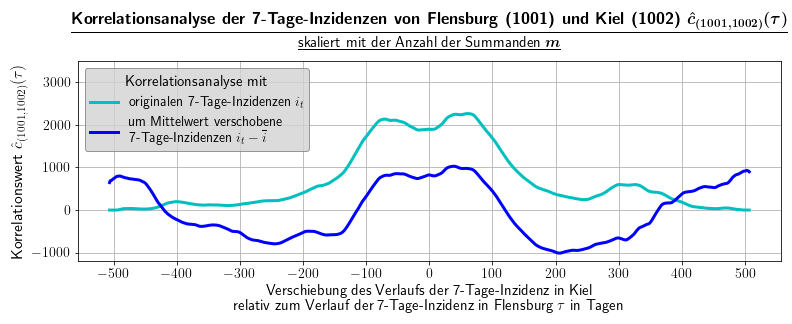
\includegraphics[width=0.95\textwidth]{figures/Grundlagen/correlation_Flensburg_Kiel_scaled_autocorrelation.png}
    \caption{Korrelationsanalyse der 7-Tages Inzidenzen der Stadtkreise Kiel und Flensburg ohne Skalierung mithilfe der Autokorrelation.
    In Hellblau ist das Ergebnis der Korrelationsanalyse mit den originalen 7-Tages Inzidenzen dargestellt. Das Ergebnis der Korrelationsanalyse mit den 7-Tages Inzidenzen, von denen der Mittelwert der 7-Tages Inzidenzen des jeweiligen Landkreises abgezogen wurde, ist blau dargestellt.}
    \label{fig:correlation_Flensburg_Kiel_scaled_autocorrelation}
\end{figure}
In \autoref{fig:correlation_Flensburg_Kiel_scaled_autocorrelation} sind die Ergebnisse der kompletten Korrelationsanalyse abgebildet, wie sie mithilfe von \autoref{eq:skalierte_Korrelation} erzeugt werden.
\begin{figure}[H]
    \centering
    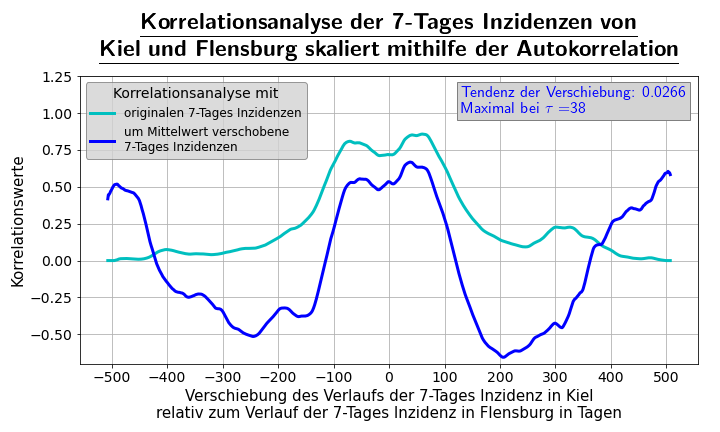
\includegraphics[width=0.95\textwidth]{figures/Grundlagen/correlation_Flensburg_Kiel_scaled_complete.png}
    \caption{Vollständige Korrelationsanalyse der 7-Tages Inzidenzen der Stadtkreise Kiel und Flensburg skaliert mithilfe der Autokorrelation.
    In Hellblau ist das Ergebnis der Korrelationsanalyse mit den originalen 7-Tages Inzidenzen dargestellt. Das Ergebnis der Korrelationsanalyse mit den 7-Tages Inzidenzen, von denen der Mittelwert der 7-Tages Inzidenzen des jeweiligen Landkreises abgezogen wurde, ist blau dargestellt.}
    \label{fig:correlation_Flensburg_Kiel_scaled_complete}
\end{figure}

In \autoref{fig:correlation_Flensburg_Kiel_scaled_complete} ist zu erkennen, das die Korrelationsanalyse von zwei Zeitserien mit 508 7-Tages Inzidenzen 1015 Korrelationswerte ergibt.
Für jeden der 412 Landkreis ergeben sich daher aus der Korrelationsanalyse mit sich selbst und jedem anderen Landkreise 418.180 Werte, ebenso ergeben sich für jeden der 38 Regierungsbezirk 38.570. Dies ergibt in Summe $
%38.570\cdot 38 + 418.180\cdot412 =
1.465.660+172.290.160=173.755.820$ Werte.

Jeder Wert gibt die Wahrscheinlichkeit einer Korrelation bei der jeweiligen Verschiebung an, wobei die zugeordneten Verschiebungen von links nach rechts bei jedem Schritt um eins zunehmen und der mittlerste der Korrelationswerte der Verschiebung $\tau = 0$ zugeordnet ist. Die Verschiebung ist im Kontext dieser Arbeit stets in ganzen Tagen zwischen $-507$ und $507$ angegeben. Der Wert an Position 501 in der Liste der Korrelationswerte gibt also an, wie wahrscheinlich der Verlauf der 7-Tages Inzidenz des ersten Gebiets mit dem um eine Woche nach links verschobenen Verlauf der 7-Tages Inzidenz des zweiten Gebiets korreliert.

\subsection{Komprimierung und Darstellung als Matrizen}\label{sec:Grundlagen:Korrelation:Komprimierung}
Das Ziel der nachfolgend beschriebenen Schritte ist, die Korrelationswerte eines Gebiets auf einen Wert zusammenzuführen. Dadurch kann man einfach und schnell auffallende Korrelationen zwischen zwei oder mehreren Gebieten finden kann.
Hierfür werden zwei verschiedenen Methoden verwendet:
\begin{itemize}
    \item Die Verschiebung mit dem maximalen Korrelationswert: Die zeitliche Verschiebung, bei der die Korrelationsanalyse den größten Wert angibt. Sie sagt aus bei welcher Verschiebung in Tagen am wahrscheinlichsten eine Korrelation vorliegt.
    \item Die Tendenz der Verschiebung: 
    Das Mittel der Differenz zwischen den Werten der betragsmäßig gleichen Verschiebungen.
    Das Resultat ermöglicht eine grobe Einschätzung, ob der maximale Wert nur ein Ausreißer ist oder nicht.
\end{itemize}

Die Berechnung der Tendenz der Verschiebung ist etwas komplexer und wird daher ebenfalls am Beispiel der Korrelationsanalyse der Stadtkreise Kiel und Flensburg erklärt.
In \autoref{fig:Flensburg_Kiel_Verschiebung_Tendenz} ist die Berechnung graphisch dargestellt.
Die Tendenz der Verschiebung berechnet sich aus der Liste der Korrelationswerte $C:\vert C\vert =m$, genauer gesagt aus ihrer Länge $m$ und ihren Werten $c_\tau$,$ -\lfloor m/2 \rfloor\geq \tau\leq \lfloor m/2 \rfloor$:
\begin{equation}
    s_{Tendenz} = \frac{1}{\lfloor m/2 \rfloor}
    \sum_{\tau=1}^{\lfloor m/2 \rfloor}c_{\tau}-c_{-\tau}
\end{equation}
In \autoref{fig:Flensburg_Kiel_Verschiebung_Tendenz} entspricht der blaue Graph den Werten der Korrelationsanalyse, wie sie auch in \autoref{fig:correlation_Flensburg_Kiel_scaled_complete} abgebildet sind. Um bildlich die Differenz zwischen den Werten der betragsmäßig gleichen Verschiebungen darzustellen, werden die Werte der negativen Verschiebungen an der Vertikalen bei $x=0$ gespiegelt und Lila eingefärbt.
Da die Linke Seite gespiegelt wird, ist sie nicht weiter von Bedeutung.

In den Zwischenräumen der beiden Graphen und auf der Horizontalen bei $y=0$ sind die Differenzen der Werte der betragsmäßig gleichen Verschiebungen aufgezeichnet, deren Mittel der Tendenz der Verschiebung entspricht. Diese ist als dunkelblaue Horizontale bei $y=0,0266$ dargestellt.

\begin{figure}[H]
    \centering
    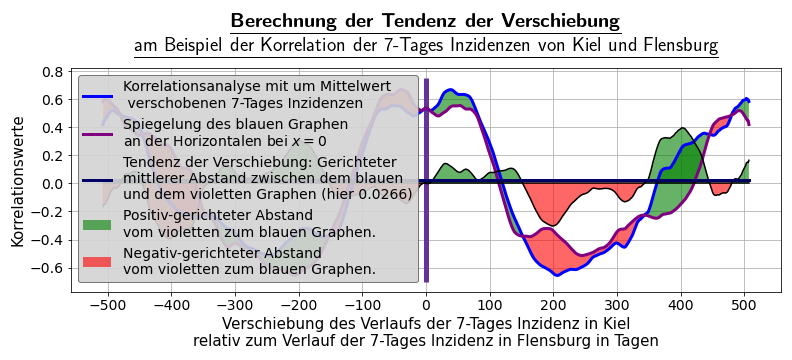
\includegraphics[width=0.95\textwidth]{figures/Grundlagen/correlation_Flensburg_Kiel_Verschiebung_Tendenz.png}
    \caption{Graphische Darstellung der Berechnung der Tendenz der Verschiebung.}
    \label{fig:Flensburg_Kiel_Verschiebung_Tendenz}
\end{figure}

Somit lässt sich zum einen die Verschiebung mit dem maximalen Korrelationswert ermitteln und einfach interpretieren.
Da hierfür jedoch nur ein Wert herausgenommen wird, bietet es sich zum anderen an, die Tendenz der Verschiebung zu berechnen und mit der Verschiebung mit dem maximalen Korrelationswert zu vergleichen.



Um dies für alle Landkreise und Regierungsbezirke zu ermöglichen, werden die beiden Werte jeweils in einer Matrix dargestellt: Jeder Zeile und Spalte wird der Index für ein Gebiet zugeordnet. In die Zellen werden entweder die Verschiebungen mit dem maximalen Korrelationswert oder die Tendenzen der Verschiebung eingetragen. Ein spezifischer Wert in einer Zelle stammt aus der Korrelationsanalyse der Gebiete, die der Zeile und der Spalte zugeordnet sind.
Die Matrizen sind (mit umgekehrtem Vorzeichen) symmetrisch an der Diagonalen von links oben nach rechts unten. Die Diagonalen sind mit Nullen besetzt, da die Werte der positiven Verschiebung symmetrisch zu den Werten der negativen Verschiebung sind und die Korrelation mit sich selbst trivialerweise bei einer Verschiebung von $\tau=0$ am größten ist, da die Werte und Trends komplett identisch sind.

Um den Gebieten selbst Werte zuzuordnen und nicht nur in Kombination mit einem anderen Gebiet, wird sowohl bei den Maximalwerten wie auch den Tendenzen der Verschiebung der Mittelwert gebildet, indem die Zeilen der Matrizen aufsummiert werden und durch die Anzahl der Spalten geteilt werden.
\section{Farbgebung}\label{sec:Grundlagen:Farbgebung}
Um schnell verständliche Abbildungen bereitstellen zu können, werden die Werte skaliert und die Farbgebung der Deutschlandkarten derart angepasst, dass das gesamte Farbspektrum abgedeckt wird. Das Farbspektrum reicht gemäß den Farben des Regenbogens von blau über grün zu gelb zu rot, wie in \autoref{fig:color_schemes} demonstriert. Die niedrigsten Werte werden blau gefärbt.
Da manche dieser Farbwerte im Kontrast zu einem weißen Hintergrund schwer zu erkennen sind, ist der Hintergrund der meisten Abbildungen grau.

\begin{figure}[H]
    \centering
    
\includegraphics[width=0.8\textwidth]{figures/Grundlagen/color_schemes.png}
    \caption{Das Farbspektrum, in welchem sich die Darstellungen bewegen. Von links nach rechts steigen die eingegebenen Werte konstant. Der angegebene Wert wird jeweils anhand des ersten und des letzten Werten einer Referenzliste linear in diesem Spektrum verortet.}
    \label{fig:color_schemes}
\end{figure}

Die Matrizen werden durch die verwendete Programmbibliothek \glqq{}Matplotlib\grqq{} automatisch eingefärbt.
    \chapter{Vorgehensweise}\label{chap:Vorgehensweise}
Um dem im Kapitel \glqq{}\ref{chap:Motivation} Motivation\grqq{} formulierten Ziel zu folgen, muss zunächst eine Datenquelle gewählt werden.
Anschließend werden deren Daten in eine nutzbare Form übertragen.
Schlussendlich können die Informationen aus den Daten verknüpft, interpretiert und graphisch dargestellt werden.

Der mit Jupyter Notebook (\href{jupyter.org}{jupyter.org}) erstellte Programmcode findet sich in den Programmdateien im Anhang der Bachelorarbeit.

Diese Bachelorarbeit basiert teilweise auf den Vorleistungen des Bachelorprojekts zur Visualisierung der COVID-19-Daten von Leander Marius Bürkin.
Ziel dieses Bachelorprojekts war eine Reihe an Deutschlandkarten in einem Video zusammenzufassen, welches die Ausbreitung der COVID-19-Pandemie in Deutschland vom ersten März 2020 bis zum letzten Tag, für den die API des Robert Koch-Instituts Daten liefert, darstellt.


Das Bachelorprojekt sowie eines der Videos ist verfügbar unter\\
\href{https://github.com/leanderbuerkin/Bachelorprojekt/blob/master/media/germany_incidence_V4_300ms_1080p_music.mp4}{https://github.com/leanderbuerkin/Bachelorprojekt/blob/master/media/}\\
\href{https://github.com/leanderbuerkin/Bachelorprojekt/blob/master/media/germany_incidence_V4_300ms_1080p_music.mp4}{germany\_incidence\_V4\_300ms\_1080p\_music.mp4}

\section{Datenquellen - Ursprung und Abspeicherung}\label{sec:Datenquelle}

Das gannnte Bachelorprojekt sowie diese Bachelorarbeit verwenden Informationen zur COVID-19-Pandemie und den geographischen Daten von 412 deutschen Landkreisen. Alle Daten stammen von der Programmierschnittstelle (API) des Robert Koch-Instituts \glqq{}COVID-19 Datenhub\grqq{}
(\href{npgeo-corona-npgeo-de.hub.arcgis.com}{npgeo-corona-npgeo-de.hub.arcgis.com}) oder werden aus den daher stammenden Daten generiert. Diese Datenquelle wurde gewählt, weil sie vom Robert Koch-Institut (RKI, \href{www.rki.de}{www.rki.de}) und dem deutschen Staat\\
 (www.bundesregierung.de) referenziert wird. Beispielsweise unter:
\begin{itemize}
    \item \href{www.bundesregierung.de/breg-de/themen/coronavirus}{www.bundesregierung.de/breg-de/themen/coronavirus}
    \item \href{www.rki.de/DE/Content/InfAZ/N/Neuartiges_Coronavirus/Daten/Fallzahlen_Inzidenz_aktualisiert.html}{www.rki.de/DE/Content/InfAZ/N/Neuartiges\_Coronavirus/Daten/Fallzahlen}\\
    \href{www.rki.de/DE/Content/InfAZ/N/Neuartiges_Coronavirus/Daten/Fallzahlen_Inzidenz_aktualisiert.html}{\_Inzidenz\_aktualisiert.html}
\end{itemize}

Insgesamt werden drei verschiedene Datenpakete der API verwendet, zum einen die geographischen Daten der Landkreise, zum anderen die Summe aller aufgetretenen COVID-19-Fälle seit Beginn der Pandemie für jeden Landkreis und jeden Tag vom 01.03.2020 bis zum 21.07.2021 sowie eine Auflistung aller Meldungen der Gesundheitsämter, in welchen das  Referenzdatum, das Meldedatum, die Anzahl der betroffenen Menschen und deren Zustand (entweder genesen, verstorben oder noch infektiös) angegeben werden. Das Referenzdatum kann laut RKI als Tag der Infektion interpretiert werden, das Meldedatum als Genesungsdatum beziehungsweise Sterbedatum \autocite{RKI_Bulletin}.

Alle drei Datenpakete liefern Daten für die deutschen Landkreise. Diese sind jeweils in Form des sogenannten Gemeindeschlüssels referenziert, eine vollständige Zuordnung der Landkreise sindet sich in \autoref{tab:counties_by_admunitid}. Die Gemeindeschlüssel bestehen aus vier oder fünf Ziffern, wobei die erste oder die ersten beiden das Bundesland angeben, die zweite bzw. dritte Stelle gegebenenfalls den Regierungsbezirk und die letzten beiden Stellen bestimmen den Landkreis. Somit lassen sich die Landkreise in Regierungsbezirke einteilen und mithilfe der Kennzahlen der Landkreise die Kennzahlen der Regierungsbezirke berechnen.

Die Landkreise, welche das RKI angibt, stimmen nicht mit den Landkreisen des Statistischen Bundesamtes  \autocite{statistischesBundesamtLandkreise}
überein: In den Daten des RKIs gibt es 118 Landkreise mehr, beziehungsweise wenn man die kreisfreien Städte abzieht, zwölf Landkreise mehr. Diese Diskrepanz kommt durch die Aufteilung von Berlin in seine 12 Bezirke. Zudem wird Eisenach in den Daten des RKIs als eigene kreisfreie Stadt gewertet und nicht zum Wartburgkreis hinzugezählt. Der Stadtkreis Eisenach ist mit dem Gemeindeschlüssel 16056 versehen. Trotz dieser Unterschiede und obwohl auch kreisfreie Städte miteinbegriffen sind, wird im folgenden weiterhin der Begriff \glqq{}Landkreise\grqq{} für alle 412 Gebiete verwendet.

Der Gemeinde
%Liste der NUTS-Codes Gemeindeschlüssel leiten sich daraus ab. URL siehe Kommentar
%https://eur-lex.europa.eu/legal-content/DE/TXT/PDF/?uri=CELEX:32016R2066&from=EN
Die Regierungsbezirke, welche sich aus den ersten zwei oder drei Stellen des Gemeindeschlüssels ergeben, stimmen leider auch nicht mit den Regierungsbezirken des Statistischen Bundesamtes
\autocite{statistischesBundesamtRegierungsbezirke}
überein: Die Gemeindeschlüssel haben 38 verschiedene Präfixe, wohingegen laut statistischem Bundesamt aktuell nur 19 Regierungsbezirke existieren.
Da jedoch nicht alle Bundesländer in Regierungsbezirke unterteilt sind, wird in neun Fällen das Bundesland an Stelle möglicher Regierungsbezirke verwendet. Die Diskrepanz von neun weiteren Gebieten entsteht durch die Veränderung der Regierungsbezirke seit der Einführung der Gemeindeschlüssel: Die Gemeindeschlüssel Niedersachsens lassen auf 4 Regierungsbezirke schließen, die Gemeindeschlüssel der Rheinland-Pfalz auf 3 und die Gemeindeschlüssel Sachsens auf 3 weitere. Keines dieser Bundesländer ist aktuell noch in Regierungsbezirke unterteilt. Somit ergeben sich 19 echte Regierungsbezirke, 10 ehemalige sowie 9 Bundesländer ohne Regierungsbezirke.
Trotz dieser Unterschiede und obwohl auch Bundesländer miteinbegriffen sind, wird im folgenden weiterhin der Begriff \glqq{}Regierungsbezirk\grqq{} für alle 38 Gebiete verwendet.

Die genannten Daten werden abgespeichert, damit sie nicht bei jeder Ausführung erneut angefordert und aufbereitet werden müssen.
\section{Datenaufbereitung}
Bevor die Daten genutzt werden können, müssen sie verifiziert werden, überflüssige Informationen entfernt werden und neue Kennzahlen aus den gegebenen Informationen berechnet werden. Daten vor der Datenaufbereitung, welche direkt von der API oder einem Backup davon stammen, werden als \glqq{}unmodifizierte\grqq{} Daten bezeichnet. 

Daten, die rudimentär auf Vollständigkeit überprüft wurden, aus den Daten generierte Daten enthalten und bei welchen überflüssige Informationen entfernt wurden, werden \glqq{}modifizierte\grqq{} Daten genannt.

Zunächst werden die unmodifizierten Daten in eine übersichtlichere Form übertragen und es wird sichergestellt, dass gleich viele Werte für jeden Landkreis vorhanden sind. Zudem werden die Umrisse der 100 Landkreise von Hand geprüft, welche mehrere Polygone enthalten, diese werden entweder als Ausschnitt oder als reale Fläche interpretiert. Würde man einfach alle Polygone zeichnen, kann es passieren, das ein Bereich, welcher komplett von einem Landkreis umgeben ist von einem seiner Polygone übermalt wird, welches genau diese Fläche aus dem Landkreis ausschneiden sollte.

Nachdem die unmodifizierten Daten in eine übersichtlichere Form übertragen und überprüft wurden, werden aus den Daten weitere Werte berechnet.

Die Bevölkerungsdichte der Landkreise wird berechnet, indem die Anzahl der Einwohner durch die Fläche in Quadratmetern geteilt wird (siehe \autoref{eq:Bevölkerungsdichte}). Beide Informationen werden von der API bereitgestellt.
Die Bevölkerungsdichte wird auch für die Regierungsbezirke berechnet. 
Sowohl die Bevölkerungsdichten der Landkreise wie auch die Bevölkerungsdichten der Regierungsbezirke werden zur Einordnung der Korrelationsanalysen auf einer Deutschlandkarte dargestellt, wobei die Farbe die Bevölkerunsdichte repräsentiert, wie in \autoref{sec:Grundlagen:Farbgebung} beschrieben.

Für jeden Landkreis und jeden Regierungsbezirk wird eine Zeitreihe mit den 7-Tage-Inzidenzen angefertigt, welche die 7-Tage-Inzidenz nach \autoref{eq:7-Tages_Inzidenz} für jeden Tag enthält, für den eine Fallzahlen angegeben ist. 

Um die Auflistung aller Meldungen der Gesundheitsämter nutzen zu können, müssen diese erst für jeden Landkreis und jeden Tag gesammelt und aufsummiert werden:
Das Referenzdatum wird als Tag der Infektion interpretiert. Die Anzahl der betroffenen Individuen wird für jeden folgenden Tag zur akkumulierten Anzahl der Fälle hinzuaddiert.
Das Meldedatum wird als Tag der Genesung beziehungsweise Tag des Todes interpretiert, je nachdem ob die Meldung Genesung oder Tod angibt. Die Anzahl der betroffenen Individuen wird hier zum einen für jeden folgenden Tag zur akkumulierten Anzahl der Genesenen/Verstorbenen hinzuaddiert. Zum anderen wird die Anzahl der betroffenen Individuen für jeden Tag zwischen dem Referenzdatum und dem Meldedatum zu den aktiven Fällen hinzuaddiert.

Mithilfe der Gesamtbevölkerung eines Landkreises werden aus diesen Daten für jeden Tag und jeden Landkreis alle drei Kategorien des SIR-Modells berechnet:

\begin{itemize}
    \item \glqq{}susceptible\grqq{}: Die Gesamtbevölkerung des Landkreises minus die akkumulierte Anzahl der Fälle.
    \item \glqq{}infectious\grqq{}: Liegt als aktive Fälle bereits vor.
    \item \glqq{}recovered\grqq{}:
    Die Summe aus der akkumulierten Anzahl der Genesenen und der Verstorbenen. Oder die akkumulierte Anzahl der Fälle minus die aktiven Fälle. Solange zu jeder Meldung ein Referenzdatum angegeben ist, entspricht das Ergebniss der zweiten Berechnungsvariante dem der ersten.
\end{itemize}

Um ein Gefühl dafür zu bekommen, welcher Lankreis in welchem Ausmaß von der COVID-19-Pandemie getroffen wurde, wird die akkumulierte Anzahl der COVID-19-Fälle des letzten Tages durch die Bevölkerung des Landkreises geteilt und farblich in einer Deutschlandkarte dargestellt.
%
\section{Datenformat}\todo{Muss entweder noch umgeschrieben werden, wodurch es sehr lang wird oder massiv gekürzt werden. Ich warte noch auf Antwort von meinem Betreuer, Korrekturleser können bei 3.4 Datendarstellung weitermachen}
Die Daten liegen in einer Kombination aus sogenannten Python Dictionaries und sogenannten Python Listen vor.

Ein Dictionary ist dadurch charakterisiert, dass man über den Namen eines Elements (\glqq{}Key\grqq{}) das Element (\glqq{}Value\grqq{}) bekommt, ähnlich wie man früher in Telefonbüchern anhand des Namens (Key) die Telefonnummer (Value) erhalten hat.

Listen sind dadurch charakterisiert, dass sie Elemente in einer fixen Reihenfolge enthalten und sich diese durch ihren Index leicht auffindbar machen. So sind beispielsweise die Anzahl der COVID-19-Fälle der einzelnen Tage chronologisch in einer Liste gespeichert, sodass man daraus direkt eine Abbildung erstellen kann.


Die Programmdateien erstellen drei verschiedene sogenannte globale Dictionaries, welche (in untergeordneten Dictionaries und Listen) alle Daten enthalten. Globale Dictionaries sind in allen Dateien verfügbar und unterscheiden sich insofern von lokalen Dictionaries/Listen, welche nur in einzelnen Programmabschnitten vorliegen und daher nicht derart zentral sind.
Die drei Dictionaries heißen
\begin{itemize}
    \item covid19
    \item counties\_geography
    \item non\_county\_specific\_data
    \item districts
\end{itemize}

\textbf{covid19}\\
Das Dictionary covid19 speichert die COVID-19-Fälle jedes deutschen Landkreises und die daraus berechnete sieben Tages Inzidenz sowie die um den Mittelwert der 7-Tage-Inzidenzen verminderten Inzidenzen.

Mit dem Gemeindeschlüssel eines Landkreises als Key und dem zusätzlichen Key \glqq{}cases\grqq{} erhält man die akkumulierte Anzahl an COVID-19-Fällen pro Tag des Landkreises als Liste.

Mit dem Gemeindeschlüssel eines Landkreises als Key und dem Key \glqq{}incidences\grqq{} erhält man die sieben Tages Inzidenz pro Tag des Landkreises als Liste.

Mit dem Gemeindeschlüssel eines Landkreises als Key und dem Key \glqq{}incidences\_scaled\grqq{} erhält man die sieben Tages Inzidenz pro Tag des Landkreises als Liste.

Alle drei Listen enthalten für jeden Tag seit dem 01.03.2020 bis zu dem Tag der aktuellsten Daten jeweils einen Eintrag.

Die Anzahl an COVID-19-Fällen pro Tag stammt aus dem \glqq{}COVID-19 Datenhub\grqq{}. Die sieben Tages Inzidenz wird wie in \autoref{sec:Grundlagen:7-Tage-Inzidenz} beschrieben aus den Daten vom COVID-19 Datenhub berechnet.

\todo{Aufbau des Gemeindeschlüssels erklären}
\textbf{counties\_geography}\\
Das Dictionary counties\_geography enthält zu jedem Landkreis ein Dictionary mit den folgenden Elemente:
\begin{itemize}
    \item[name:] Der Name des Landkreises
    \item[population:] Die Einwohnerzahl des Landkreis aus einer offiziellen Schätzung (nähere Informationen finden sich im COVID-19 Datenhub). Diese Zahlen werden auch für die offizielle Berechnung der sieben Tages Inzidenz verwendet.
    \item[area\_in\_m2:] Die Fläche des Landkreises in Quadratmetern
    \item[geometry:] Die Form des Landkreises in einer für die Darstellung angepassten Form
    \item[raw\_geometry:] Die Form des Landkreises in der originalen Form
    \item[population\_density:] Die Bevölkerungsdichte des Landkreises, berechnet aus der Fläche des Landkreises und seiner Einwohnerzahl
\end{itemize}
Außer die Bevölkerungsdichte, welche berechnet wird, und die angepassten Formen der Landkreise, welche aus den origialen Formen generiert werden, stammen alle Daten direkt aus dem \glqq{}COVID-19 Datenhub\grqq{}.

\textbf{non\_county\_specific\_data}
Das Dictionary non\_county\_specific\_data enthält die folgenden Elemente:
\begin{itemize}
    \item[unixtime:] Die Unixzeit, wie sie vom COVID-19 Datenhub zur Verfügung gestellt wird: Die Zahl der Millisekunden seit dem 01.01.1970 00:00 Uhr UTC. Die Zahl der COVID-19-Fälle und die sieben Tages Inzidenz eines entsprechenden Tages befinden sich an der selben Stelle in Ihrer jeweiligen Liste, wie der Tag in dieser Liste.
    \item[states:] Die Name und Nummern der deutschen Bundesländer. Die ersten beiden oder die erste Zahl des Gemeindeschlüssel eines Landkreises geben das Bundesland an, in welchem der Landkreis liegt. Die ersten zwei bzw. drei Zahlen geben den Regierungsbezirk an, in dem der Landkreis. Sollte es im jeweiligen Bundesland keine Regierungsbezirke geben, entspricht dies dem Bundesland.
    \item[highest\_case\_number:] Die höchste akkumulierte Fallzahl unter allen Landkreisen.
    \item[lowest\_case\_number:] Die niedrigste akkumulierte Fallzahl unter allen Landkreisen.
    \item[highest\_incidence:] Die höchste sieben Tages Inzidenz eines Tages unter allen Landkreisen.
    \item[lowest\_incidence:] Die niedrigste sieben Tages Inzidenz eines Tages unter allen Landkreisen.
    \item[UTC:] Die Unixzeit konvertiert in die Koordinierte Weltzeit im Format \glqq{}DD.MM.YYYY\grqq{}.
    \item[UTC+7days:] Die Liste der Zeiten gespeichert in UTC plus sieben weitere Tage vor dem erstem Datum in der Liste. Diese werden benutzt, um den Zeitraum der 7-Tage-Inzidenz der ersten sieben Tage darstellen zu können: die hierfür verwendeten Zeiträume beginnen jeweils vor dem ersten hier dokumentierten Fall.
\end{itemize}
\todo{itemize reparieren}
Die Unixzeit, die Namen und die Nummern der Bundesländer stammen aus dem \glqq{}COVID-19 Datenhub\grqq{}. Alle anderen Informationen wurden gesammelt oder berechnet.

In Abbildung \ref{fig:dicts_als_code} sind die drei Dictionaries dargestellt, wie sie auch im Programm verwendet werden.
\begin{figure}[H]
    \centering
    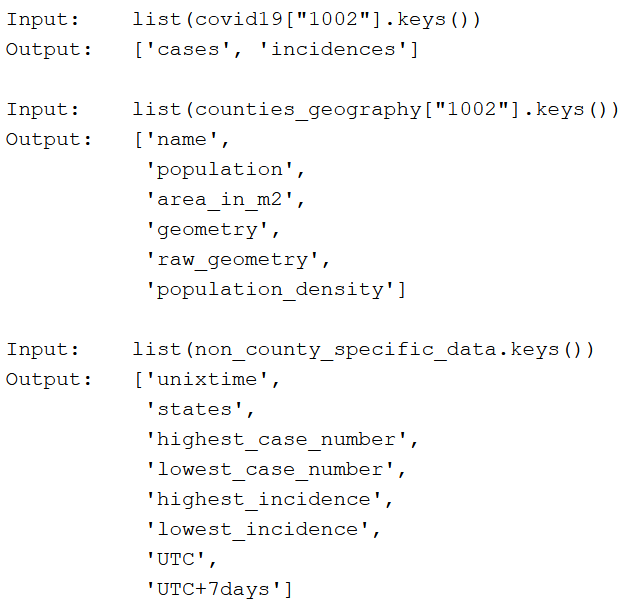
\includegraphics[width=0.8\textwidth]{figures/Vorgehensweise/Dictionarys Bachelorprojekt.png}
    \caption{
    Die Dictionaries non\_county\_specific\_data, counties\_geography und covid19 mit ihren jeweiligen Schlüsseln.
    Für die Dictionaries covid19 und counties\_geography wurde jeweils der Landkreis Kiel (Gemeindeschlüssel 1002) zur Veranschaulichung verwendet.}
    \label{fig:dicts_als_code}
\end{figure}

\todo{Daten aus Meldungen einpflegen}
\section{Datendarstellung}
Abschließend werden die Daten wie folgt dargestellt.
\subsection{Allgemeine Daten der Gebiete}
Zuerst werden die folgenden Daten der Landkreise und Regierungsbezirke dargestellt, welche auf einfachen Gleichungen beruhen und lediglich zur Einordnung der anderen Ergebnisse dienen:
\begin{itemize}
    \item Die Bevölkerungsdichte, um diese mit dem Infektionsverhalten in Zusammenhang setzen zu können.
    \item Die Anordnung der Gebiete, wenn man sie nach ihrem Gemeindeschlüssel sortiert - Die Sortierung erfolgt hier lexikographisch, das heißt, das die Länge des Gemeindeschlüssels keine Rolle spielt, sondern immer das erste Zeichen verglichen wird und bei Übereinstimmung das nächste verglichen wird. Dadurch ergibt sich eine einheitlichere Nord-Süd-Aufteilung als die Sortierung nach dem Betrag.
    \item Die Summe der 7-Tage-Inzidenzen als Maß dafür, wie stark ein Gebiet betroffen war.
\end{itemize}
\subsection{SIR-Modell}
Zudem wird anhand der Daten ein SIR-Modell erstellt.


Da jedoch die Zahl der aktiven Fälle sehr niedrig und dementsprechend sensibel gegenüber kleinen Anomalien sind, wird dieses nur auf Bundesebene erstellt. 
Hierfür werden die drei Kennzahlen des SIR-Modells in drei Abbildungen dargestellt.
\subsection{Korrelationsanalyse}
Für alle Korrelationsanalysen werden aus den in \autoref{sec:Grundlagen:7-Tages Inzidenz} genannten Gründen die 7-Tage-Inzidenzen nach \autoref{eq:7-Tages_Inzidenz} verwendet. Folgenden Gebiete werden nach den in \autoref{sec:BeschreibungKorrelationsanalyse} beschriebenen Methoden untersucht:
\begin{itemize}
    \item Die Korrelation der in \autoref{fig:selected_counties} dargestellten Landkreise mit den Stadtkreisen, die sie umgeben, siehe \autoref{sec:selected_counties}
    \item Die Korrelationen aller Landkreise untereinander
    \item Die Korrelationen aller Regierungsbezirke untereinander
\end{itemize}

\begin{figure}[H]
    \centering
    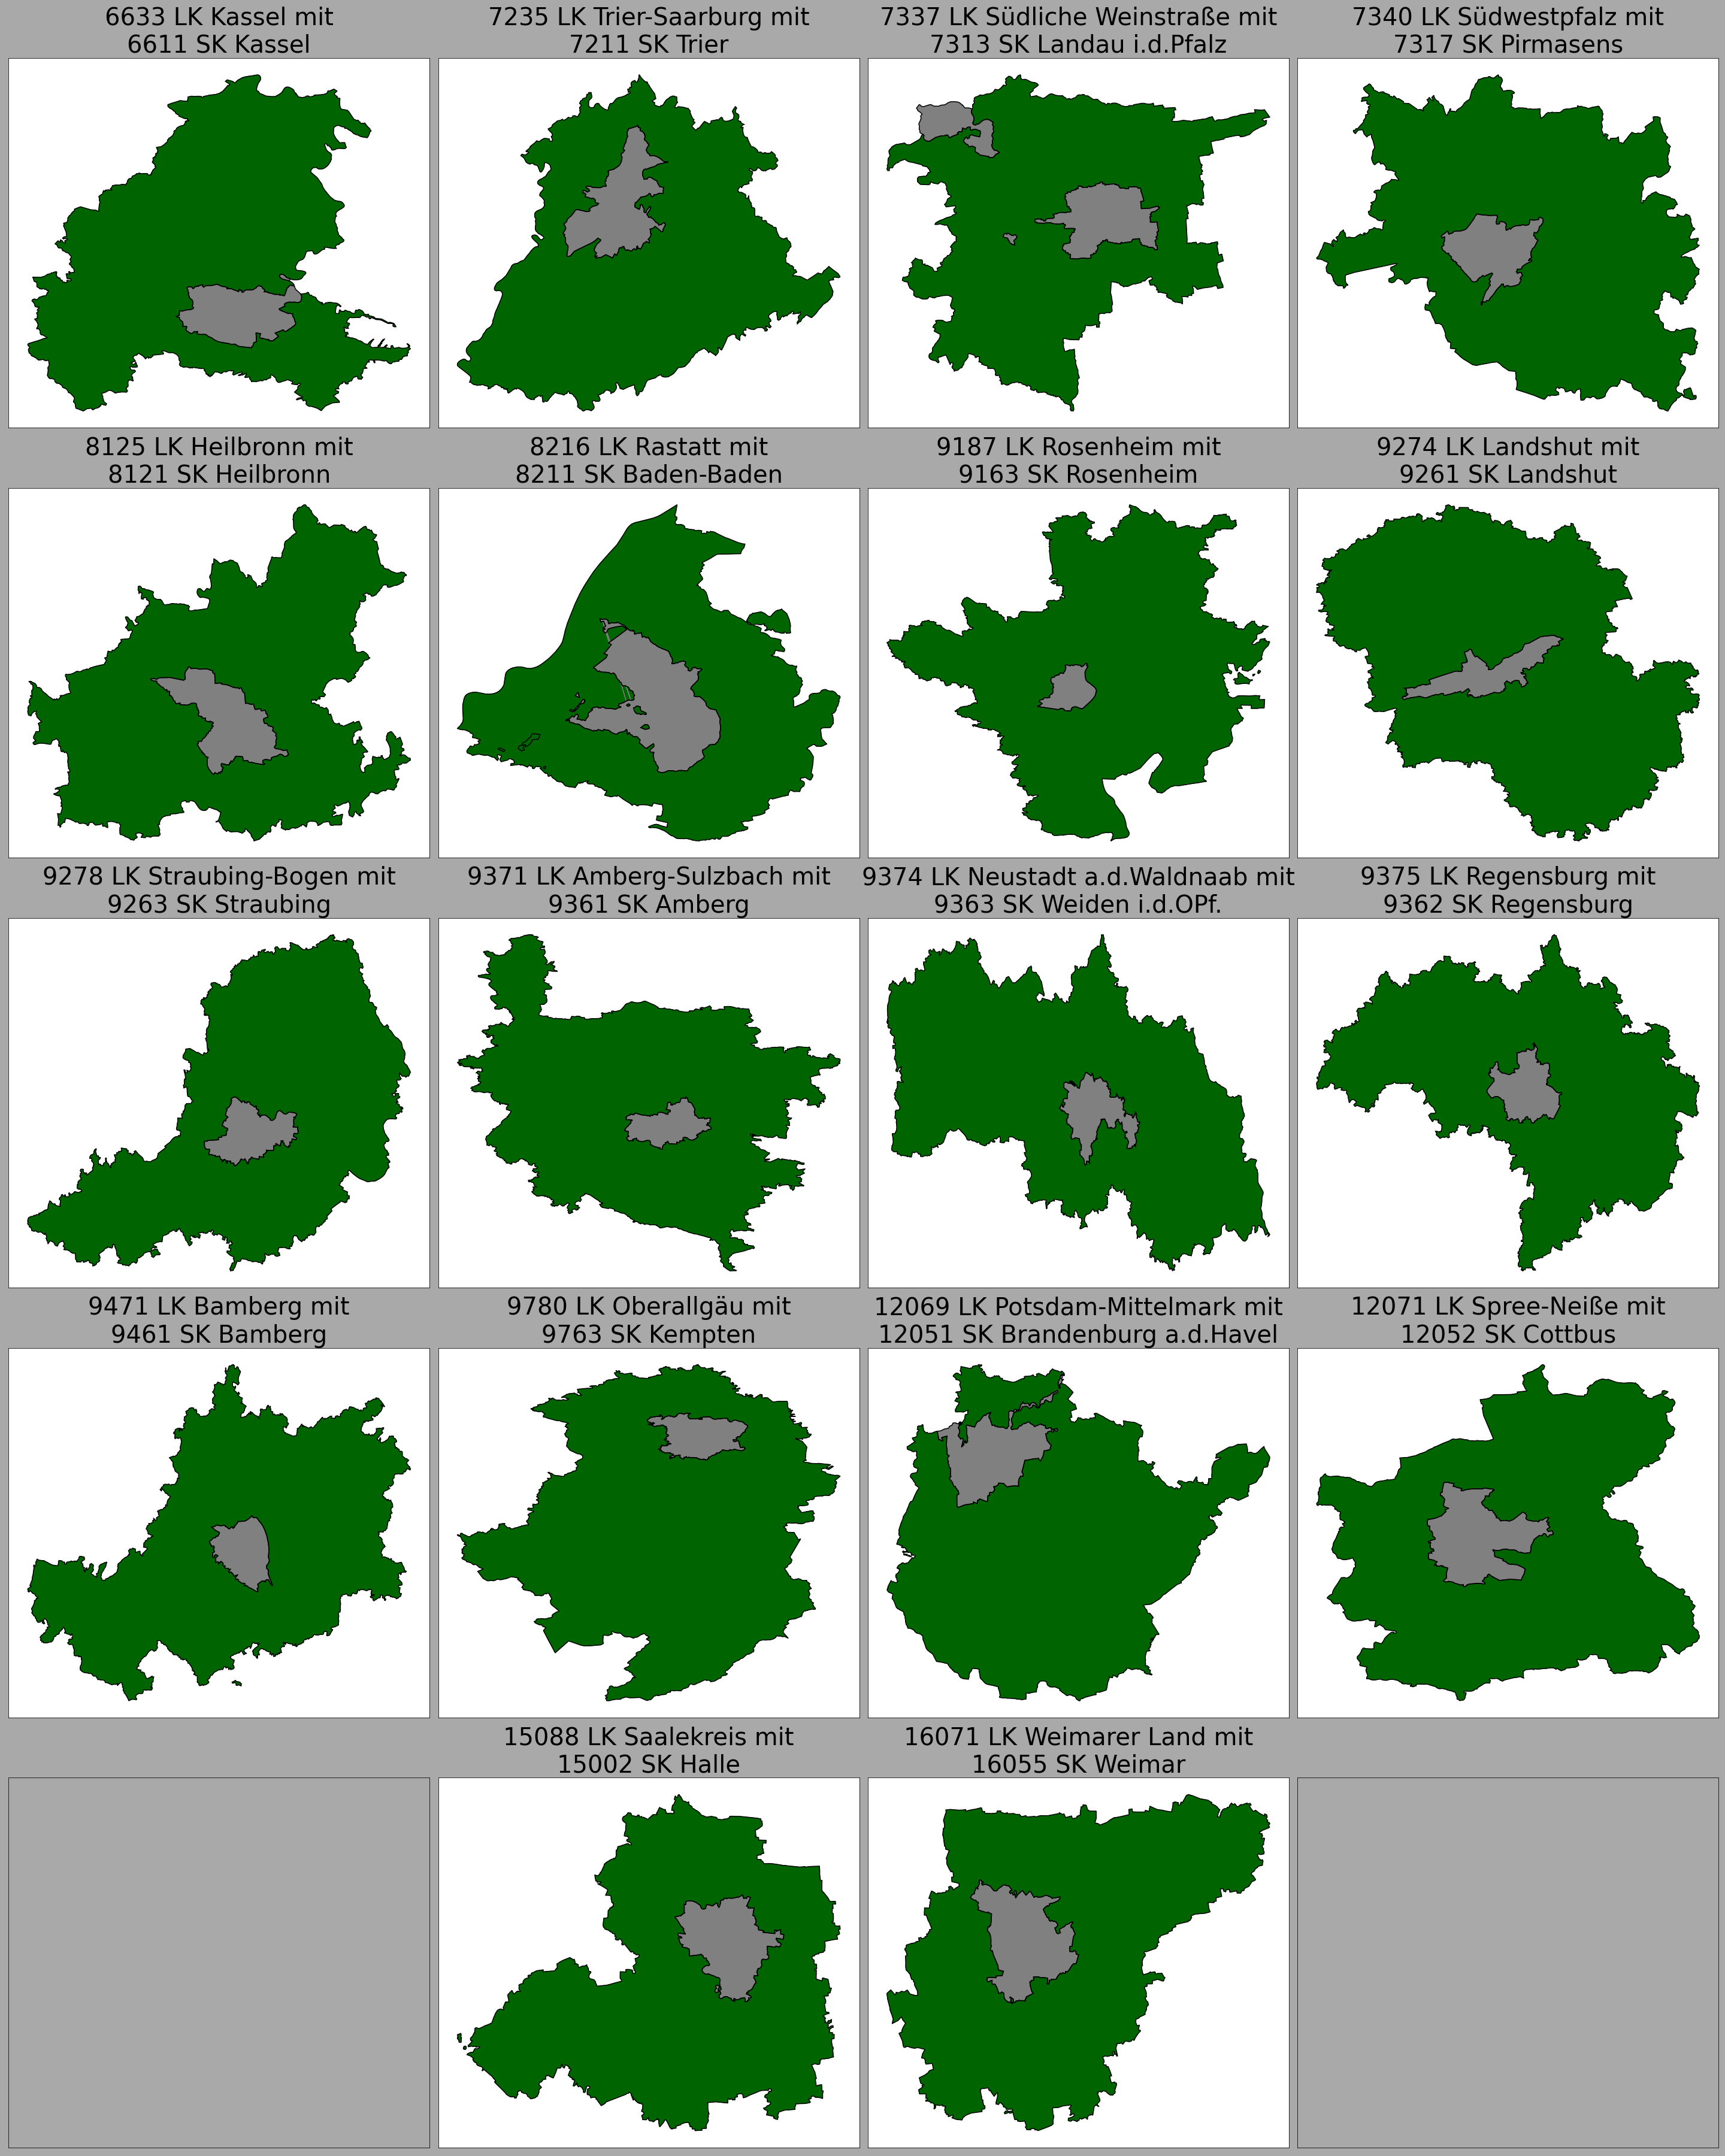
\includegraphics[width=\textwidth]{figures/Vorgehensweise/selected_counties.png}
    \caption{Die ausgewählten Landkreise mit den Stadtkreisen, die sie jeweils umgeben. In Grün jeweils der Landkreis und in Dunkelgrau der Stadtkreis, der umschlossen wird.}
    \label{fig:selected_counties}
\end{figure}
In dieser Arbeit werden nur Korrelationen mit einem zeitlichen Versatz zwischen $\tau=-50$ und $\tau=50$ betrachtet, da zum einen eine Interpretation für eine Verschiebung von mehr als 50 Tagen sehr schwierig ist und zum anderen einzelne Ausreißer bei größeren Verschiebungen stärker ins Gewicht fallen, weil immer weniger Produkte aufsummiert werden. Dies fällt auch in \autoref{fig:correlation_Flensburg_Kiel_scaled_autocorrelation} im Vergleich zu \autoref{fig:correlation_Flensburg_Kiel} an den Rändern der Graphen auf.

Um ein detailliertes Bild zu erhalten, werden zudem Korrelationsanalysen für die Verschiebungen $\tau\in[-30,30]$ und $\tau\in[-14,14]$ durchgeführt.

\subsection{Korrelation einzelner ausgewählter Städte und Landkreise}\label{sec:selected_counties}
Zum Einstieg werden die Korrelationen zwischen den Landkreisen aus \autoref{fig:selected_counties} und den Stadtkreisen, die sie umgeben, berechnet.
An ihnen lässt sich besonders gut testen, ob sich in den Korrelationswerten zwischen einer Stadt und ihrem Umland eine zeitliche Verschiebung feststellen lässt.
Um die festgestellten zeitlichen Verschiebungen einzuordnen, wird zudem ermittelt, bei wieviel Prozent der Korrelationen aller deutschen Landkreise untereinander der höchste Korrelationswert bei einer Verschiebung von $\tau = 0$ zu finden ist.

Für die ausgewählten Landkreis-Stadtkreis-Paare werden Korrelationsanalysen durchgeführt, wie in \autoref{sec:BeschreibungKorrelationsanalyse} beschrieben. Da es sich um eine übersichtliche Datenmenge handelt und für jedes Gebiet nur eine Korrelation geprüft wird, werden die Werte, welche normalerweise in Matrixform dargestellt werden, explizit ausgegeben.
\subsection{Korrelationsanalysen aller Landkreise und Regierungsbezirke}\label{sec:Vorgehensweise:Korrelationsanalysen aller Landkreise und Regierungsbezirke}


    \chapter{Resultate}\label{chap:Durchführung}
\section{Korrelationsanalysen}
Im folgenden werden die Korrelation der Corona-Fälle der einzelnen deutschen Landkreise untersucht.
%\section{Datenquelle}
\section{Datenaufbereitung}\label{sec:Datenaufbereitung}
\section{Darstellung der Daten}\label{sec:Darstellung der Daten}
\section{Bevölkerungsdichten der Landkreise}
Zuallererst folgen die genutzten Daten, welche nichts mit Corona zutun haben: Die Landkreise und ihre Bevölkerungsdichte. Die Bevölkerungsdichte wird aus der Bevölkerungszahl und der Fläche des Landkreises berechnet, welche von der API bereitgestellt werden \todo{adäquate Verlinkung auf API}.

In Abbildung \autoref{fig:distribution_pop_density_counties} sind die Bevölkerungsdichten der einzelnen Landkreise dargestellt. Auf der linken Seite befindet sich die Verteilung und auf der rechten Seite die räumliche Anordnung.
Die Bezirke Berlins sind einzeln gelistet, daher entsprechen die sechs höchsten Bevölkerungsdichten den Berliner Bezirken  Friedrichshain-Kreuzberg, Mitte, Neukölln, Tempelhof-Schöneberg, Lichtenberg, Charlottenburg-Wilmersdorf, obwohl die Bevölkerungsdichte des gesamten Berliner Stadtkreises niedriger ist als die Bevölkerungsdichte Münchens (in dieser Auflistung Platz 7, ohne Berliner Bezirke Platz 1).

\begin{figure}[H]
    \centering
    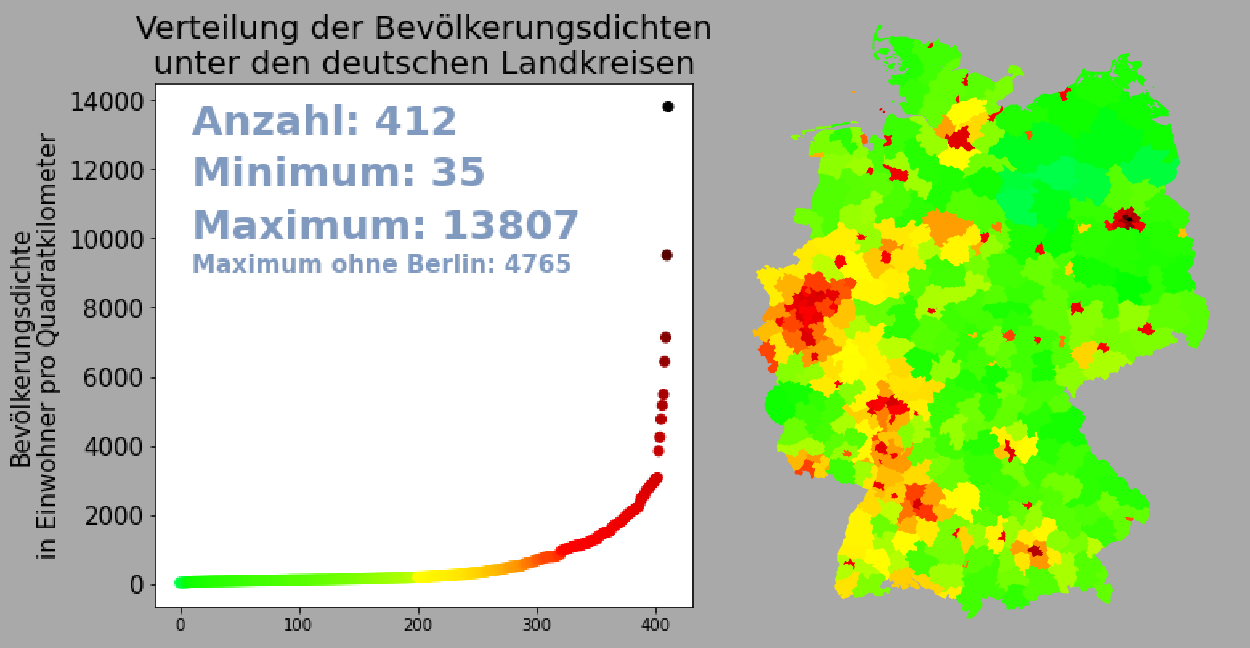
\includegraphics[width = 0.95\textwidth]{figures/Durchführung/population_density_counties_Distribution_and_map.png}
    \caption{Verteilung der Bevölkerungsdichten unter den deutschen Landkreisen.}
    \label{fig:distribution_pop_density_counties}
\end{figure}

\todo{klarstellen, das die Landkreise nicht den Landkreisen entsprechen (Berlin ist aufgeteilt) Aus Wikipedia "Landkreis": In Deutschland gibt es 294 Landkreise. Zusammen mit den 106 kreisfreien Städten bilden sie die insgesamt 400 Gebietskörperschaften auf Kreisebene. Wir haben 412.}
In Abbildung 


\begin{figure}[H]
    \centering
    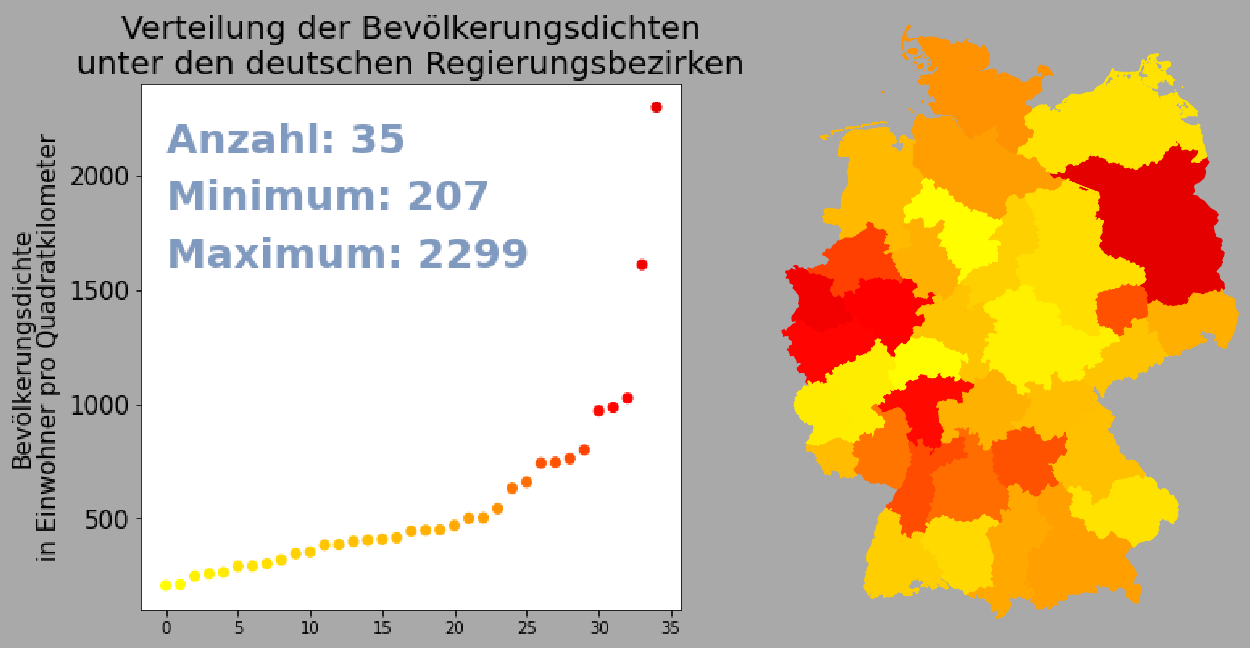
\includegraphics[width = 0.95\textwidth]{figures/Durchführung/population_density_districts_Distribution_and_map.png}
    \caption{Verteilung der Bevölkerungsdichten unter den deutschen Regierungsbezirken. Die Skalierung entspricht der Farbgebung in \autoref{fig:distribution_pop_density_counties}.}
    \label{fig:distribution_pop_density_districts}
\end{figure}

Klar zu erkennen sind die Stadtkreise in Abbildung \ref{fig:distribution_pop_density_counties}: Sie weisen eine hohe Bevölkerungsdichte auf und sind in der Regel von weniger stark bevölkerten Landkreisen umgeben.

\section{Bevölkerungsdichte der Regierungsbezirke}
Teilt man die Landkreise nach den ersten beiden Kennzahlen des Landkreises, die des Bundeslandes und die des aktuellen (teils auch vergangenen) Regierungsbezirks, ein, ergibt sich für die Bevölkerungsdichte das in \autoref{fig:distribution_pop_density_districts} dargestellte Bild.
\section{SRI-Modell}\label{sec:SRI-Modell}
\subsection{Korrelationen nach Bevölkerungsdichte}


\subsection{Die deutschen Landkreise und Ihre Bevölkerungsdichte}
Zuallererst folgen die genutzten Daten, welche nichts mit Corona zutun haben: Die Landkreise und ihre Bevölkerungsdichte. Die Bevölkerungsdichte wird aus der Bevölkerungszahl und der Fläche des Landkreises berechnet, welche von der API bereitgestellt werden \todo{adäquate Verlinkung auf API}.

In Abbildung \autoref{fig:distribution_pop_density_counties} sind die Bevölkerungsdichten der einzelnen Landkreise dargestellt. Auf der linken Seite befindet sich die Verteilung und auf der rechten Seite die räumliche Anordnung.
Die Bezirke Berlins sind einzeln gelistet, daher entsprechen die sechs höchsten Bevölkerungsdichten den Berliner Bezirken  Friedrichshain-Kreuzberg, Mitte, Neukölln, Tempelhof-Schöneberg, Lichtenberg, Charlottenburg-Wilmersdorf, obwohl die Bevölkerungsdichte des gesamten Berliner Stadtkreises niedriger ist als die Bevölkerungsdichte Münchens (in dieser Auflistung Platz 7, ohne Berliner Bezirke Platz 1).

\begin{figure}[H]
    \centering
    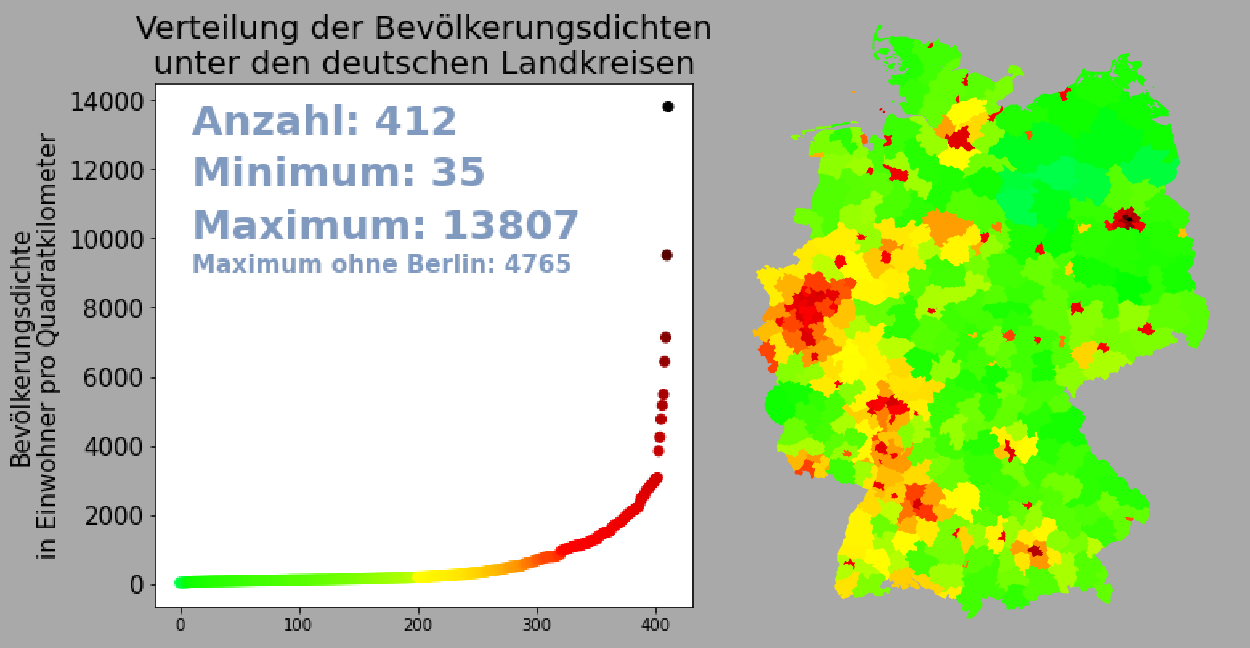
\includegraphics[width = 0.95\textwidth]{figures/Durchführung/population_density_counties_Distribution_and_map.png}
    \caption{Verteilung der Bevölkerungsdichten unter den deutschen Landkreisen.}
    \label{fig:distribution_pop_density_counties}
\end{figure}

\todo{klarstellen, das die Landkreise nicht den Landkreisen entsprechen (Berlin ist aufgeteilt) Aus Wikipedia "Landkreis": In Deutschland gibt es 294 Landkreise. Zusammen mit den 106 kreisfreien Städten bilden sie die insgesamt 400 Gebietskörperschaften auf Kreisebene. Wir haben 412.}
In Abbildung 


Teilt man die Landkreise nach den ersten beiden Kennzahlen des Landkreises, die des Bundeslandes und die des aktuellen (teils auch vergangenen) Regierungsbezirks, ein, ergibt sich für die Bevölkerungsdichte das in \autoref{fig:distribution_pop_density_districts} dargestellte Bild.

Nicht alle Bundesländer wurden in Regierungsbezirke unterteilt, in diesem Fall wird die Bevölkerungsdichte des Landkreises gewählt. Im folgenden wird dennoch von \glqq{}den Regierungsbezirken\grqq{} gesprochen. Zudem sind die Stadtstaaten Bremen und Hamburg zum Regierungsbezirk Lüneburg hinzugefügt und der Stadtstaat Berlin zum Bundesland Brandenburg hinzugefügt.

\begin{figure}[H]
    \centering
    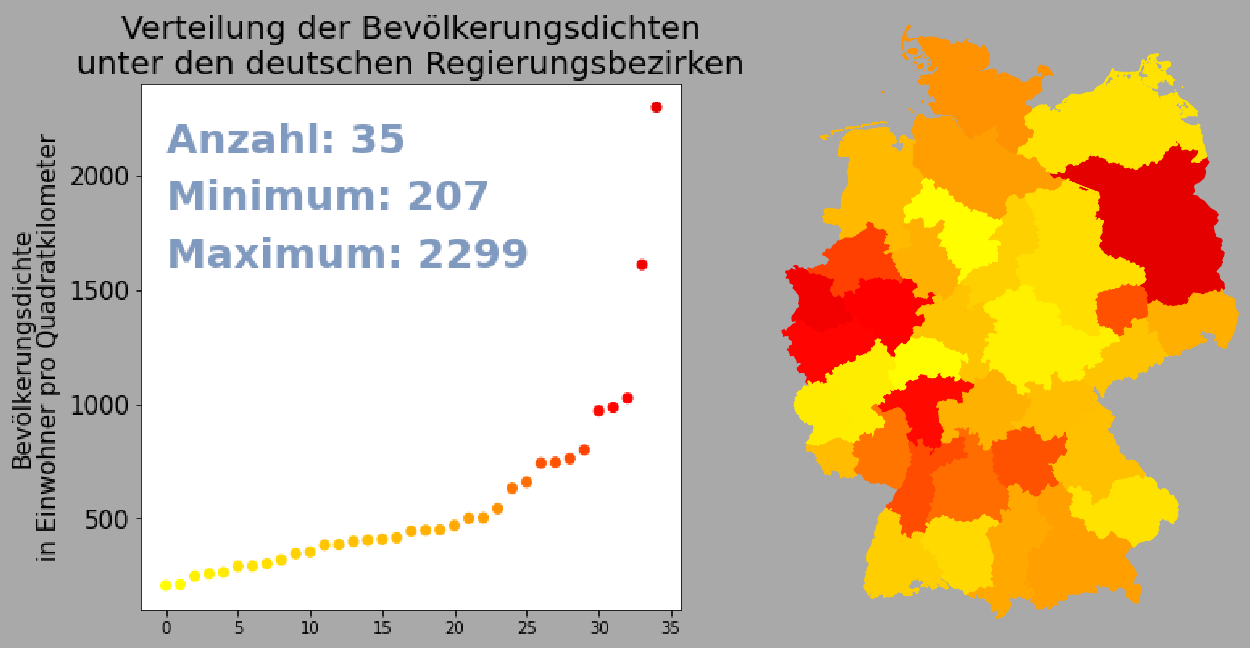
\includegraphics[width = 0.95\textwidth]{figures/Durchführung/population_density_districts_Distribution_and_map.png}
    \caption{Verteilung der Bevölkerungsdichten unter den deutschen Regierungsbezirken. Die Skalierung entspricht der Farbgebung in \autoref{fig:distribution_pop_density_counties}.}
    \label{fig:distribution_pop_density_districts}
\end{figure}

Klar zu erkennen sind die Stadtkreise in Abbildung \ref{fig:distribution_pop_density_counties}: Sie weisen eine hohe Bevölkerungsdichte auf und sind in der Regel von weniger stark bevölkerten Landkreisen umgeben.

Als erstes Beispiel zu Demonstrationszwecken ausführlich gezeigt.

Die Städte in Tabelle \ref{tab:landkreise_um_städte} von einem Landkreis umgeben, an Ihnen lässt sich besonders gut testen, ob sich in den Korrelationswahrscheinlichkeiten zwischen einer Stadt und ihrem Umland eine zeitliche Verschiebung feststellen lässt.
\begin{table}[H]
    \centering
    \begin{tabular}{c|c|c|c}
    Name des Land-&AGS &Umgebener  &AGS\\
    kreises (LK)  &Landkreis&Stadtkreis (SK)&Stadtkreis\\
    \hline
Kassel & 6633 & Kassel & 6611 \\\hdashline
Trier-Saarburg & 7235 & Trier & 7211 \\\hdashline
Südliche Weinstraße & 7337 & Landau i.d.Pfalz & 7313 \\\hdashline
Südwestpfalz & 7340 & Pirmasens & 7317 \\\hdashline
Heilbronn & 8125 & Heilbronn & 8121 \\\hdashline
Rastatt & 8216 & Baden-Baden & 8211 \\\hdashline
Rosenheim & 9187 & Rosenheim & 9163 \\\hdashline
Landshut & 9274 & Landshut & 9261 \\\hdashline
Straubing-Bogen & 9278 & Straubing & 9263 \\\hdashline
Amberg-Sulzbach & 9371 & Amberg & 9361 \\\hdashline
Neustadt a.d.Waldnaab & 9374 & Weiden i.d.OPf & 9363 \\\hdashline
Regensburg & 9375 & Regensburg & 9362 \\\hdashline
Bamberg & 9471 & Bamberg & 9461 \\\hdashline
\begin{comment}
Bayreuth & 9472 &  &  \\\hdashline
Coburg & 9473 &  &  \\\hdashline
Hof & 9475 &  &  \\\hdashline
Ansbach & 9571 &  &  \\\hdashline
Schweinfurt & 9678 &  &  \\\hdashline
Würzburg & 9679 &  &  \\\hdashline
Ostallgäu & 9777 &  &  \\\hdashline
\end{comment}
Oberallgäu & 9780 & Kempten & 9763 \\\hdashline
Potsdam-Mittelmark & 12069 & Brandenburg a.d. Havel & 12051 \\\hdashline
Spree-Neiße & 12071 & Cottbus & 12052 \\\hdashline
Saalekreis & 15088 & Halle (Saale) & 15002 \\\hdashline
Weimarer Land & 16071 & Weimar & 16055
    \end{tabular}
    \caption{Landkreise mit Name und Gemeindeschlüssel (AGS), die den jeweils mit Name und Gemeindeschlüssel gekennzeichneten Stadtkreis komplett umgeben.}
    \label{tab:landkreise_um_städte}
\end{table}

In Abbildung \autoref{fig:selected_counties} sind die ausgewählten Landkreise mit den Stadtkreisen, die sie umgeben abbgebildet.
\begin{figure}
    \centering
    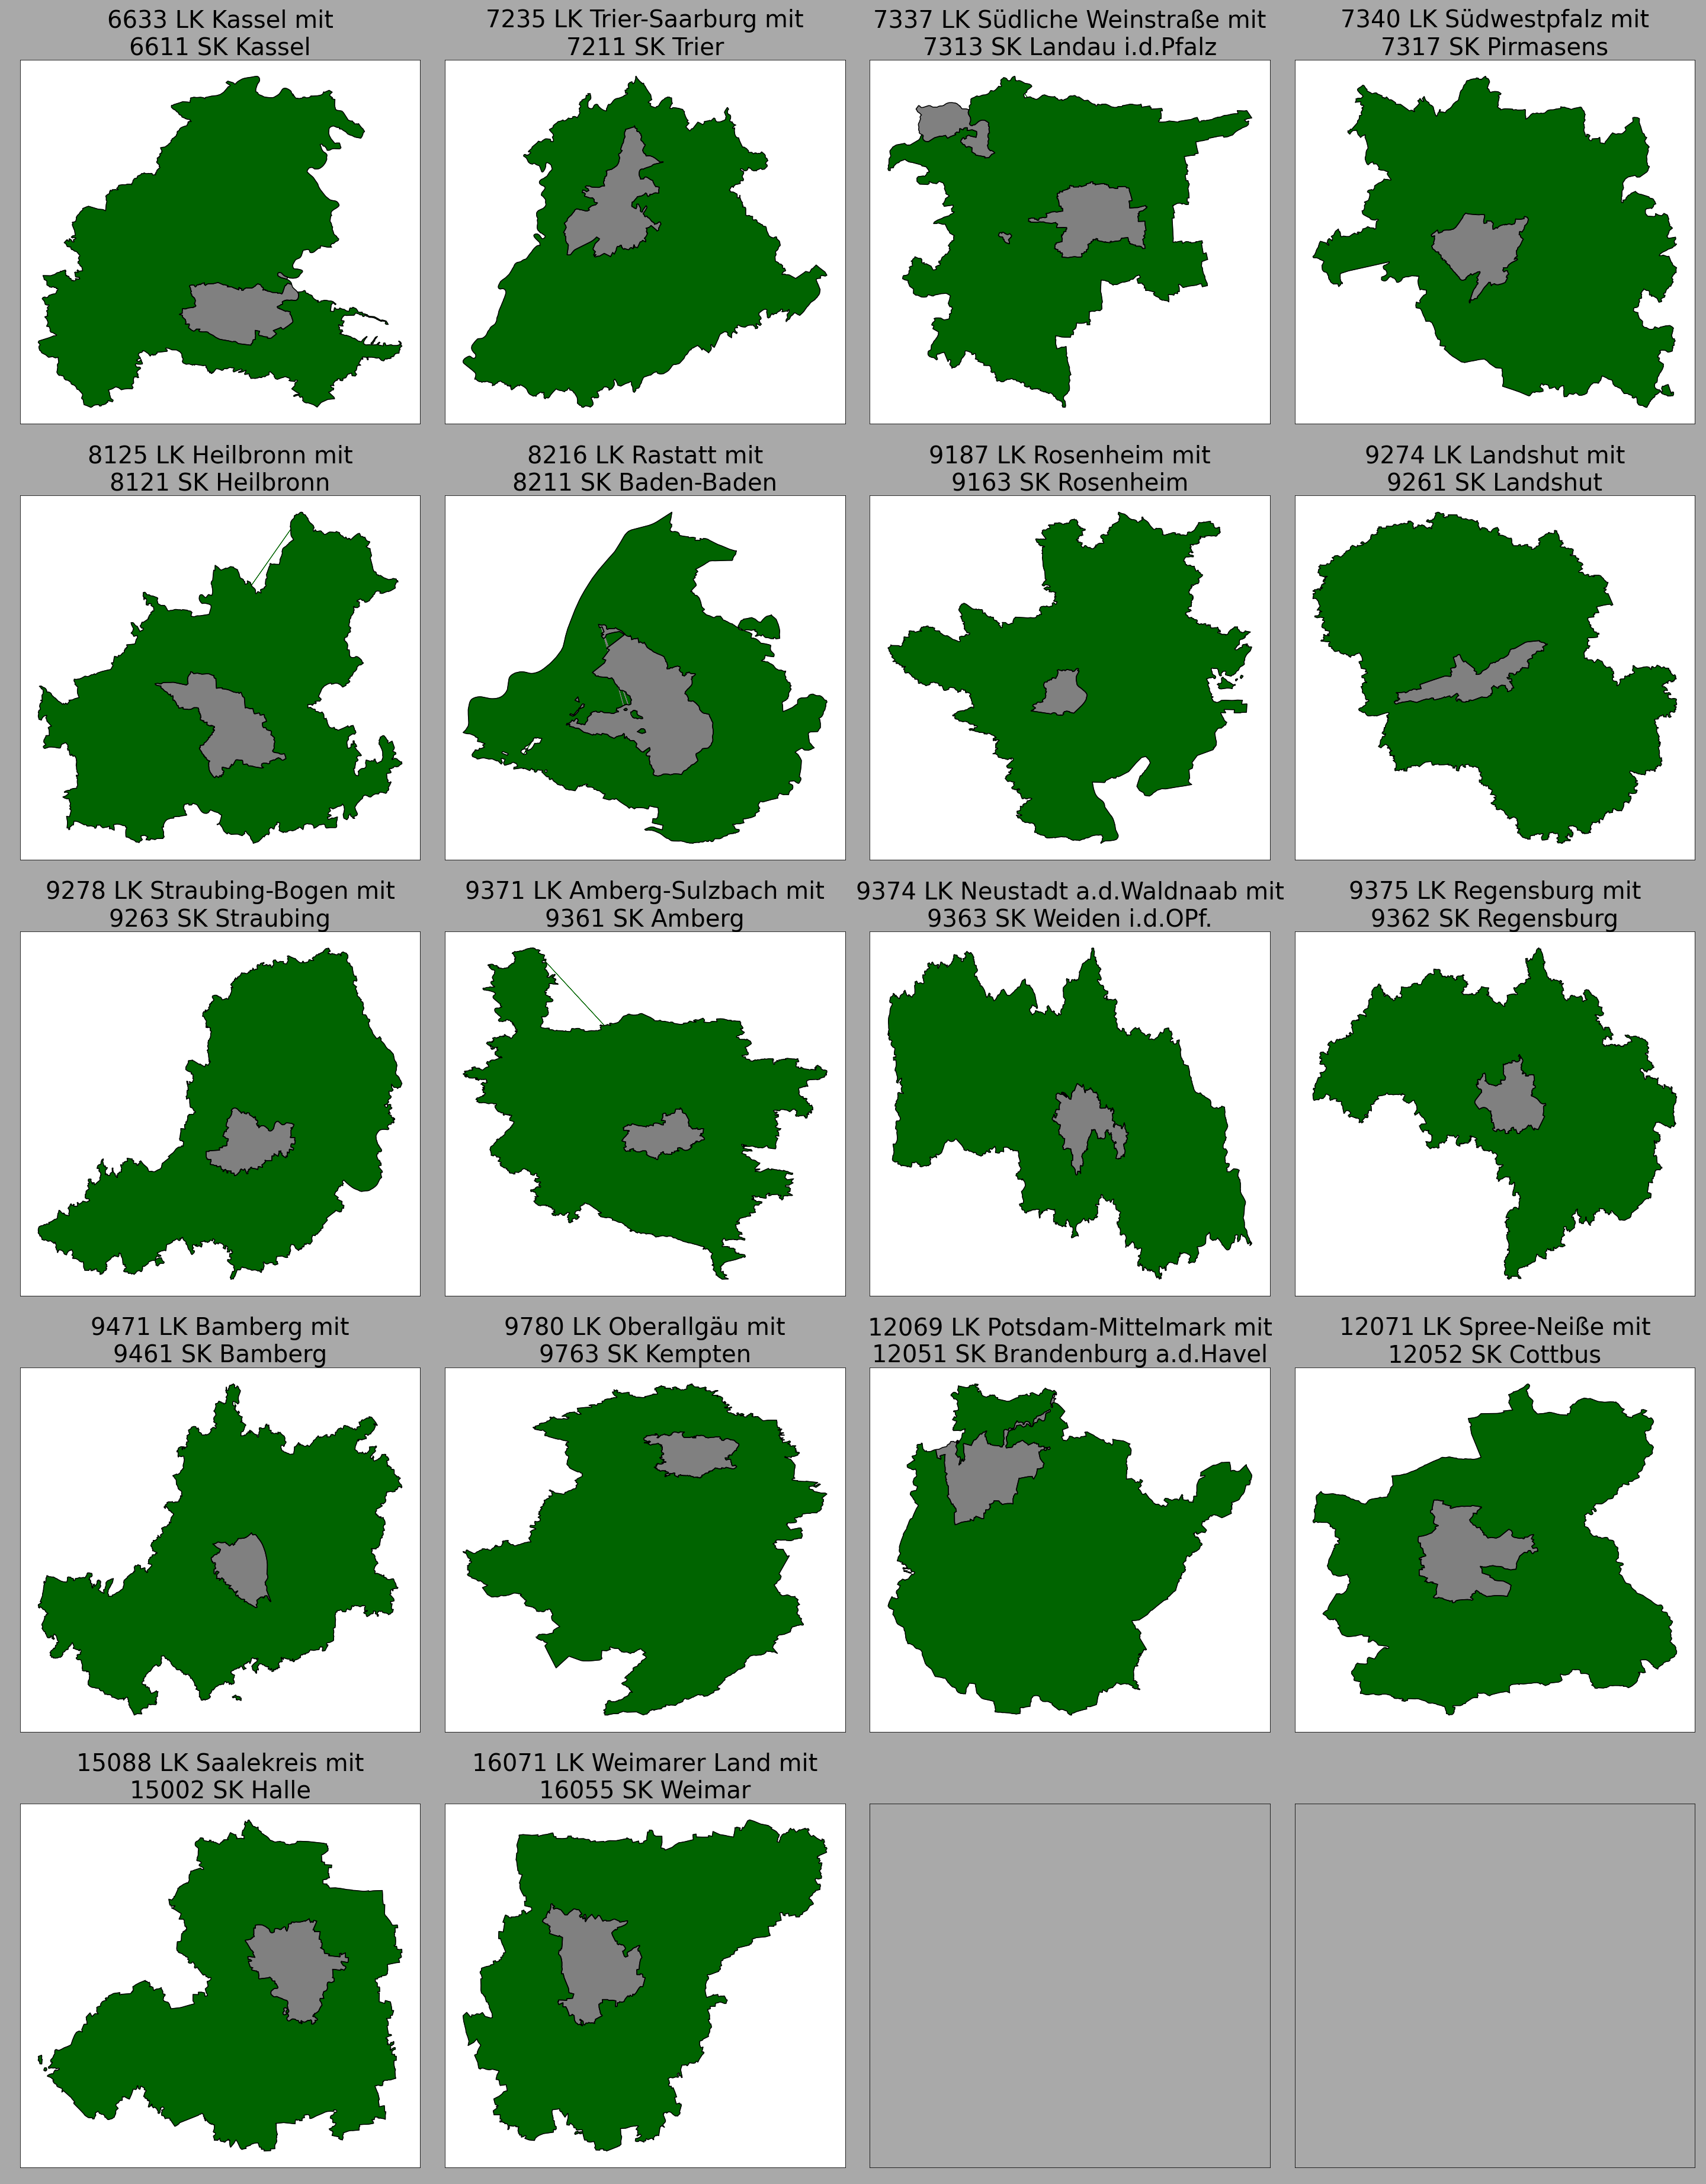
\includegraphics[width=\textwidth]{figures/Durchführung/selected_counties.png}
    \caption{Die ausgewählten Landkreise mit den Stadtkreisen, die sie jeweils umgeben.}
    \label{fig:selected_counties}
\end{figure}
    \chapter{Diskussion}\label{chap:Diskussion}
\todo{Vergleiche mit (kommentar siehe Code)}
% https://www.rki.de/DE/Content/Infekt/EpidBull/Archiv/2020/Ausgaben/17_20.pdf?__blob=publicationFile
    \chapter{Zusammenfassung}\label{chap:Zusammenfassun}
Nach den Erkentnissen dieser Arbeit scheinen Anstiege in den 7-Tages Inzidenzen der deutschen Stadtstaaten bis jetzt als Vorwarnung gut geeignet gewesen zu sein. Die vielen Anomalien wie beispielsweise das Superspreading-Event in Cloppenburg im Oktober 2020 zeigen jedoch auf, das sich diese Ausbrüche nicht an trivialen Charakteristiken der Landkreise, Regierungsbezirke oder Bundesländer festmachen lassen.

Die Meldungen der einzelnen Landkreise, welche das Robert-Koch-Institut (RKI) zur Verfügung stellt, enthalten leider sehr viele fragwürdige Meldungen (Genesungsdatum liegt vor dem Ansteckungsdatum oder außergewöhnlich lange Infektionszeiten). Da zudem die Anzahl der aktiven Fälle innerhalb einer Woche beachtlich schwankt, lässt sich aus dem SIR-Modell nicht ohne weitere Annahmen und Maßnahmen, wie sie das RKI bei seinen Berechnungen benutzt, Wissen generieren.

Die Zahl der Ansteckungen, welche täglich vom RKI herausgegeben wird eignet sich jedoch sehr gut zur Berechnung der 7-Tages Inzidenz.
Bei der Korrelation der 7-Tages Inzidenzen der deutschen Landkreise und Regierungsbezirke ergeben sich einige interessante Erkentnisse:
\begin{itemize}
    \item Die 7-Tages Inzidenzen von 18 Städten, welche von einem Landkreis komplett umgeben sind, steigen nahezu zeitgleich mit den 7-Tages Inzidenzen der Landkreise.
    \item Die Inzidenzwerte scheinen in dichter besiedelten Gebieten tendenziell früher zu steigen als in dünner besiedelten Gebieten.
    \item Einzelne Superspreading-Events können für einen signifkanten früheren Ausschlag der 7-Tages Inzidenz eines ganzen Regierungsbezirks sorgen.
    \item Die 7-Tages Inzidenzen in den neuen Bundesländern scheinen vor den 7-Tages Inzidenzen in den alten Bundesländern zu steigen, ansonsten lässt sich jedoch kein Nord-West-Verlauf oder ähnliches feststellen.
\end{itemize}
    \chapter{Danksagung}
Vielen herzlichen Dank den zahlreichen Helfern, welche mich mental und inhaltlich unterstützt haben!

Zuallererst danke ich meinem Betreuer Dr. Andreas Greiner, welcher mich vor einem Jahr mit der Idee für diese Arbeit infiziert hat und seither dieses Abenteuer mit mir gewagt hat. Er hat mich durch seine Motivation und sein Wissen auch nach tiefen Rückschlägen immer wieder dazu gebracht, weiterzumachen und neue Möglichkeiten zu finden. Vielen Dank für deine Expertise und deine höchst sympathische Art!\\
Zudem möchte ich mich bei Prof. Moritz Mathias Diehl bedanken, dass er sich mit seiner immensen Fachexpertise, in die ich durch seine Vorlesungen einen winzigen Einblick erhaschen durfte, mit meiner Bachelorarbeit befasst und sie begutachtet. Vielen Dank!

An zweiter Stelle möchte ich meinen Mitbewohnern Sarah Weitz und Sebastian Rauser danken, welchen ich meine Programme und Gedankengänge an langen Abenden erklären durfte und ich so logische Fehler korrigieren oder schwer verständliche Dinge zugänglicher machen konnte. Vielen Dank für eure Geduld und eure Wissbegierde!

Nicht zu vernachlässigen ist zudem der Beitrag meiner Familie: Im gesamten Studium boten mit meine Geschwister Elena und Fabian Bürkin Orientierung und Halt, wenn ich nicht mehr weiter wußte oder auf einem falschen Weg war. Beide konnten mir durch ihre Erfahrungen aus dem Mikrosystemtechnik- bzw. Mathematik-master einen Strauß an Tipps und Tricks mitgeben, mit denen ich theoretisch schon an meinem Master wäre, wenn ich sie richtig umgesetzt hätte. Vielen herzlichen Dank für eure Geduld mit eurem kleinen Bruder und eure Hilfsbereitschaft zu jeder Zeit!

Zu guter Letzt möchte ich meinen Kollegen, Komilitonen, Korrekturlesern und vor allem Freunden Andreas Philipp, Franz Kostelzky, Lea Hohl und Ellen Hermle bedanken, die sich durch diese Arbeit gequält haben und die mir bei Dr. Andreas Greiners teils schwierigen mathematischen Ausführungen Hoffnung gegeben haben, weil sie auch nicht alles beim ersten Mal verstanden haben. Auf einen Kaffee und vielen Dank!
    \chapter{Anhang}\label{Anhang}
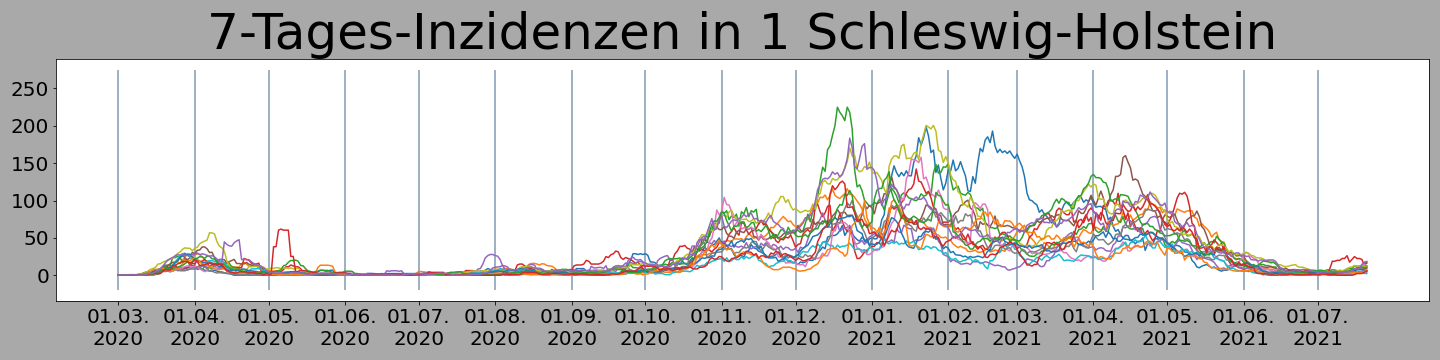
\includegraphics[width=\textwidth]{figures/Anhang/1_Schleswig-Holstein.png}
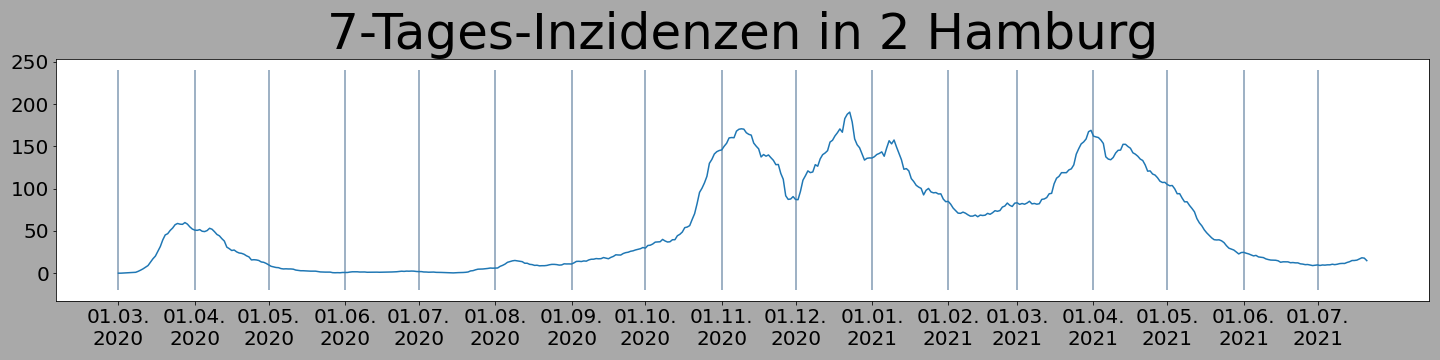
\includegraphics[width=\textwidth]{figures/Anhang/2_Hamburg.png}
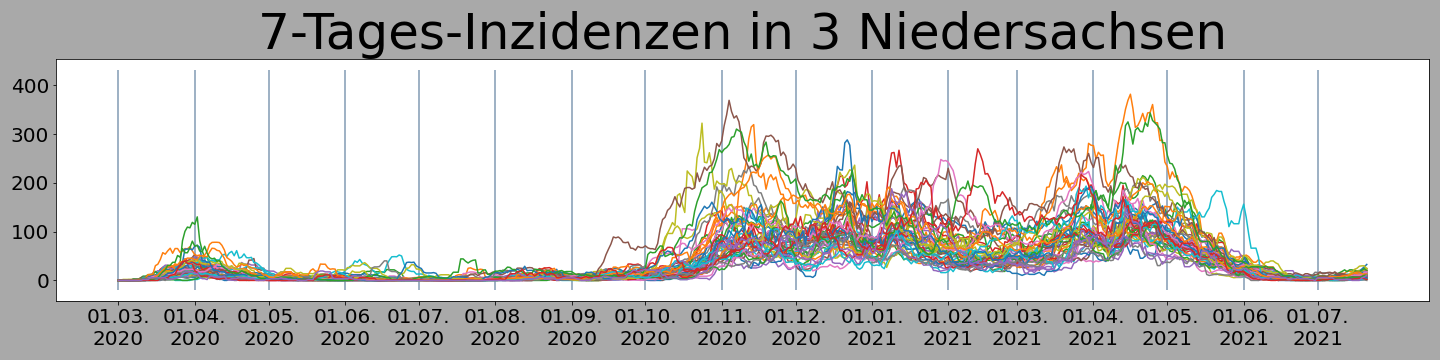
\includegraphics[width=\textwidth]{figures/Anhang/3_Niedersachsen.png}
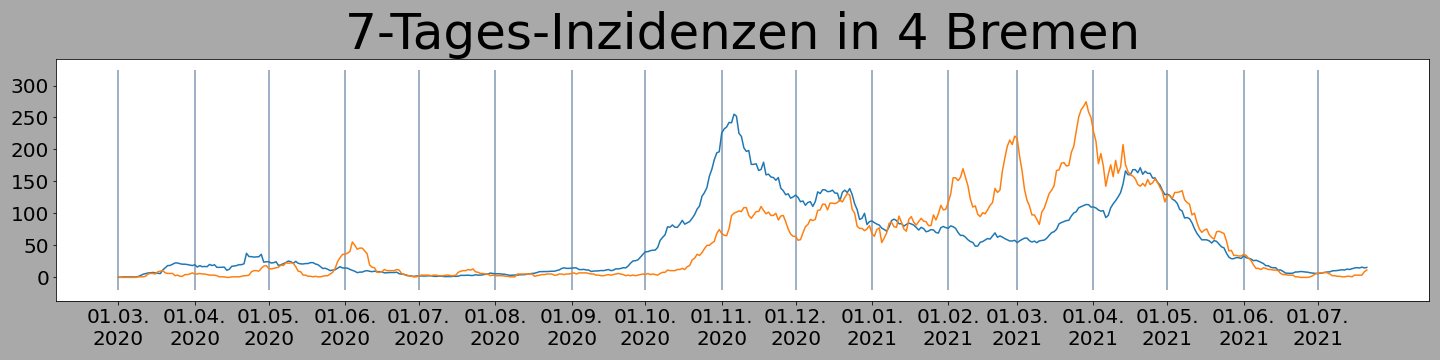
\includegraphics[width=\textwidth]{figures/Anhang/4_Bremen.png}
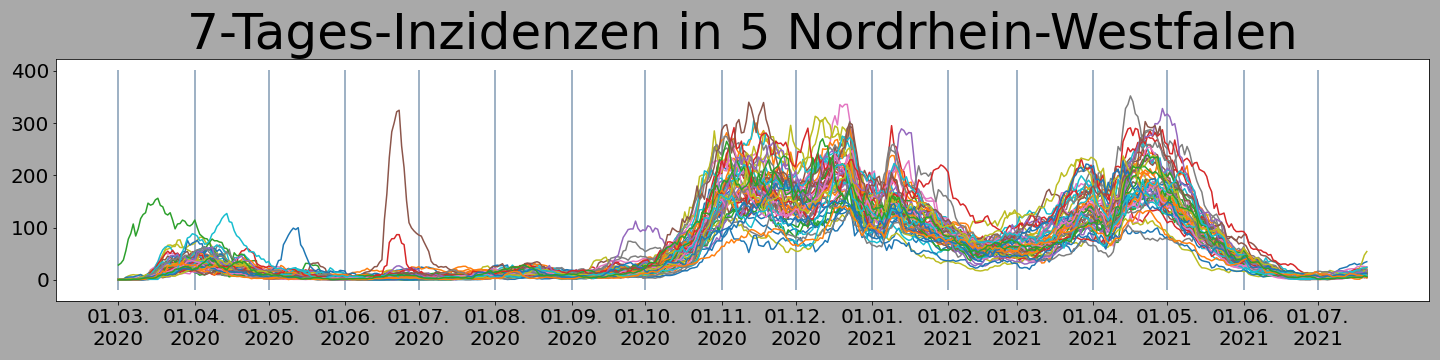
\includegraphics[width=\textwidth]{figures/Anhang/5_Nordrhein-Westfalen.png}
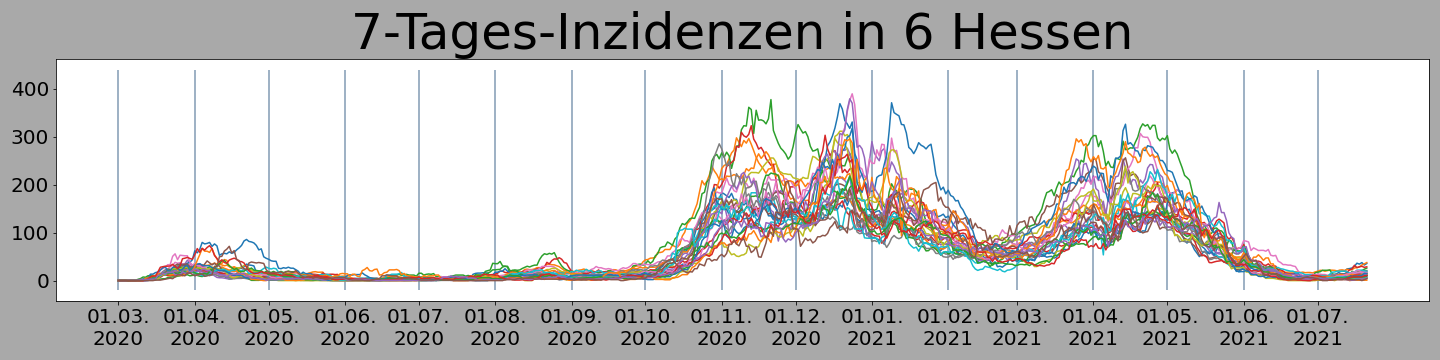
\includegraphics[width=\textwidth]{figures/Anhang/6_Hessen.png}
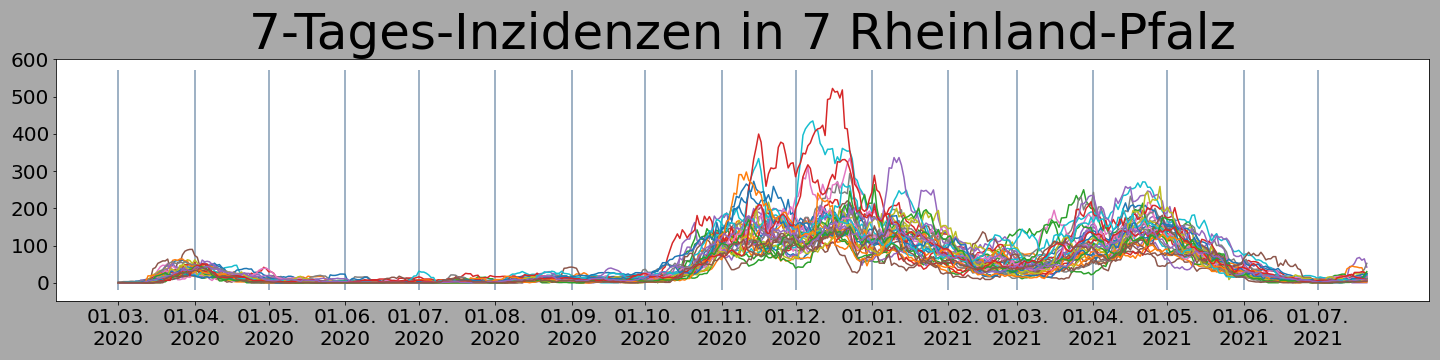
\includegraphics[width=\textwidth]{figures/Anhang/7_Rheinland-Pfalz.png}
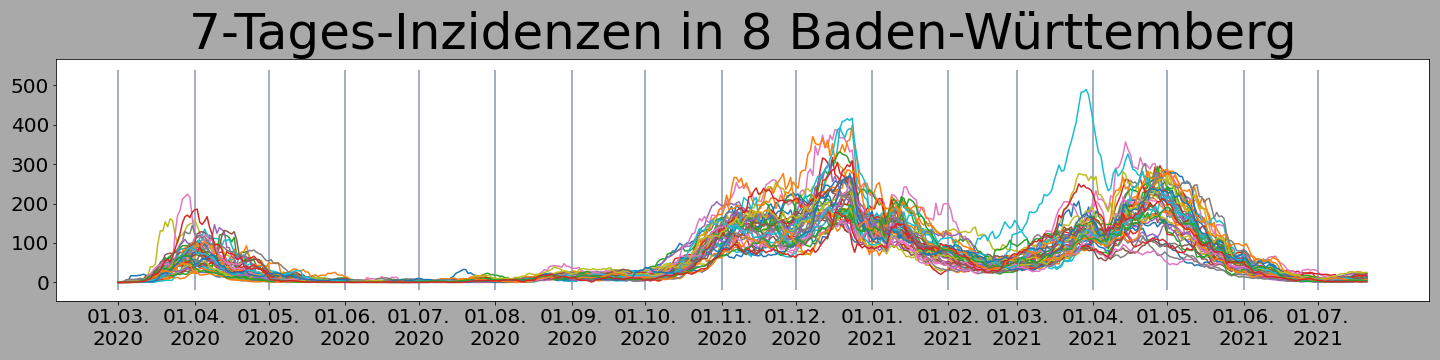
\includegraphics[width=\textwidth]{figures/Anhang/8_Baden-Württemberg.png}
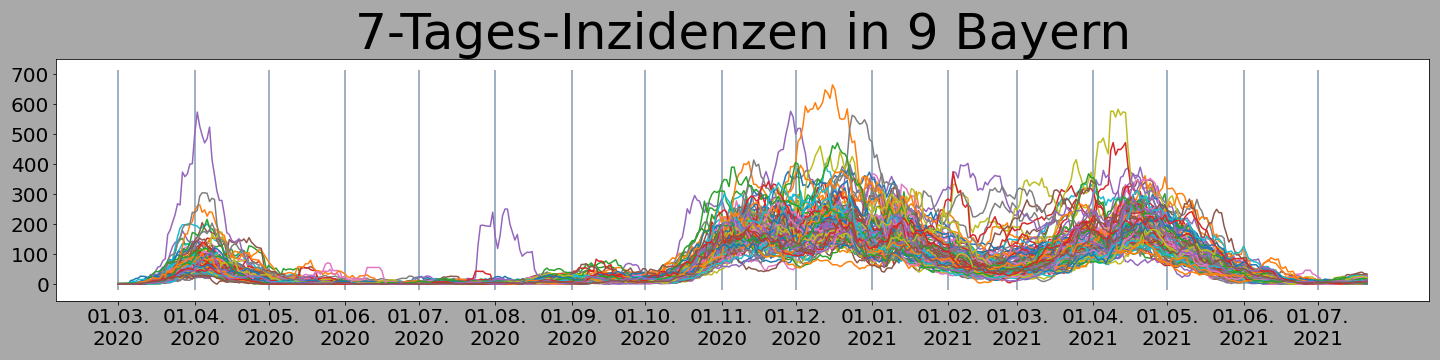
\includegraphics[width=\textwidth]{figures/Anhang/9_Bayern.png}
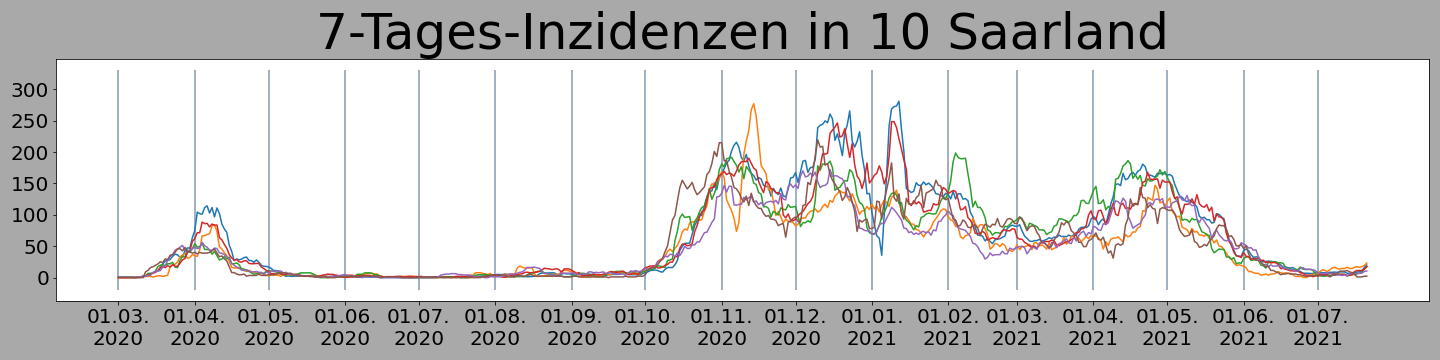
\includegraphics[width=\textwidth]{figures/Anhang/10_Saarland.png}
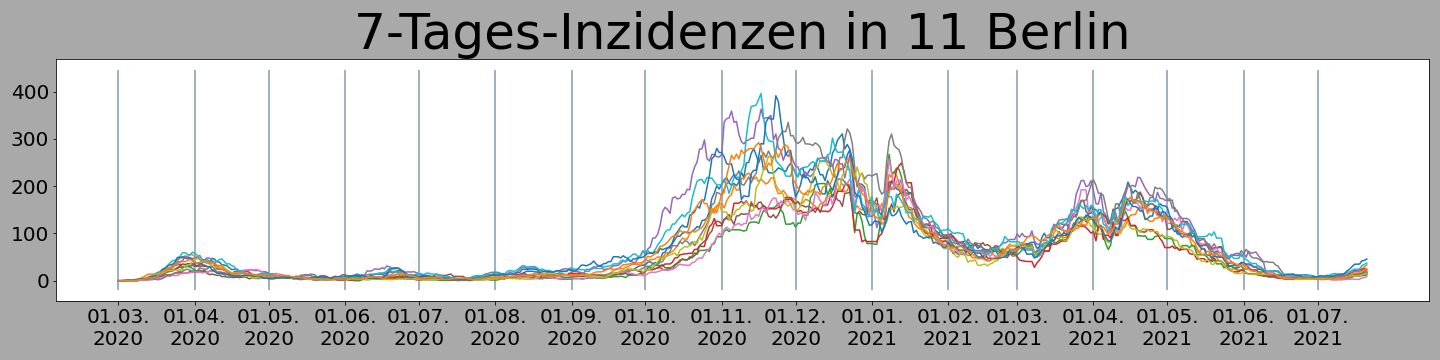
\includegraphics[width=\textwidth]{figures/Anhang/11_Berlin.png}
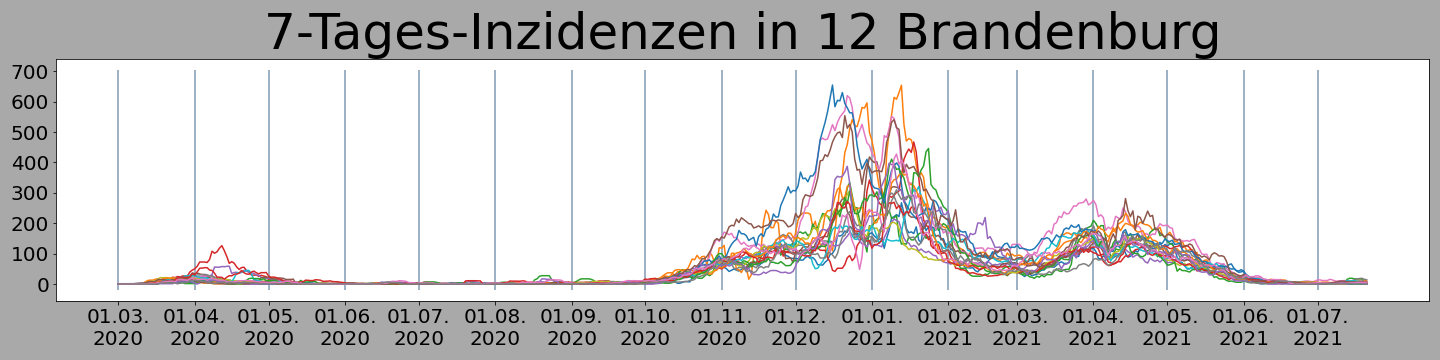
\includegraphics[width=\textwidth]{figures/Anhang/12_Brandenburg.png}
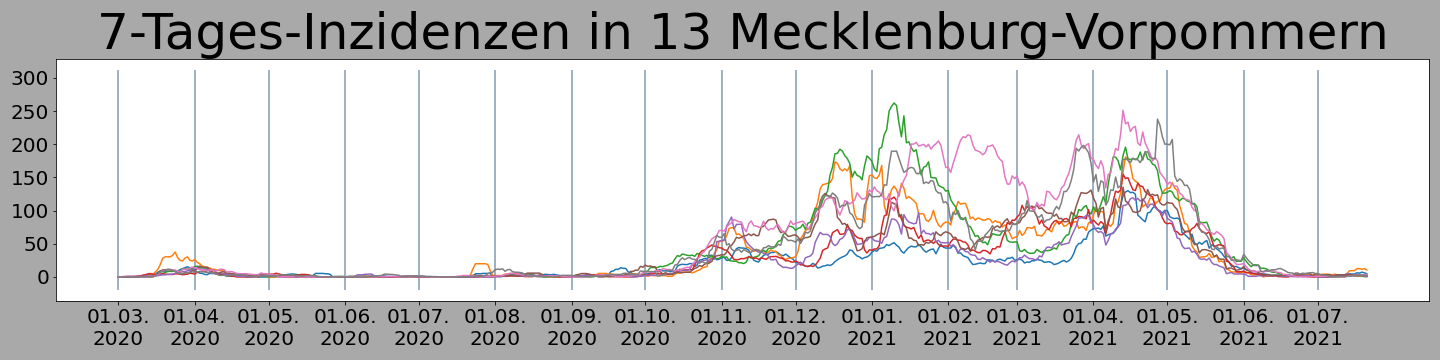
\includegraphics[width=\textwidth]{figures/Anhang/13_Mecklenburg-Vorpommern.png}
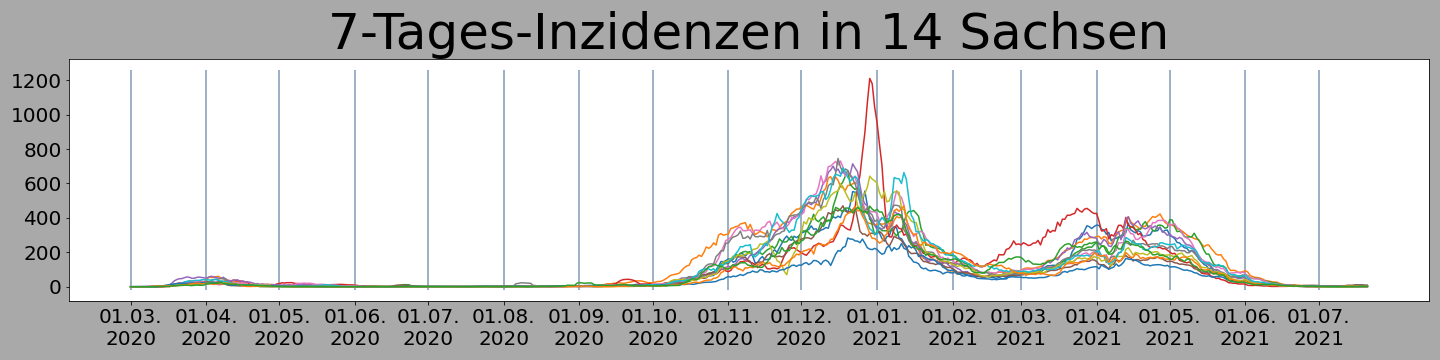
\includegraphics[width=\textwidth]{figures/Anhang/14_Sachsen.png}
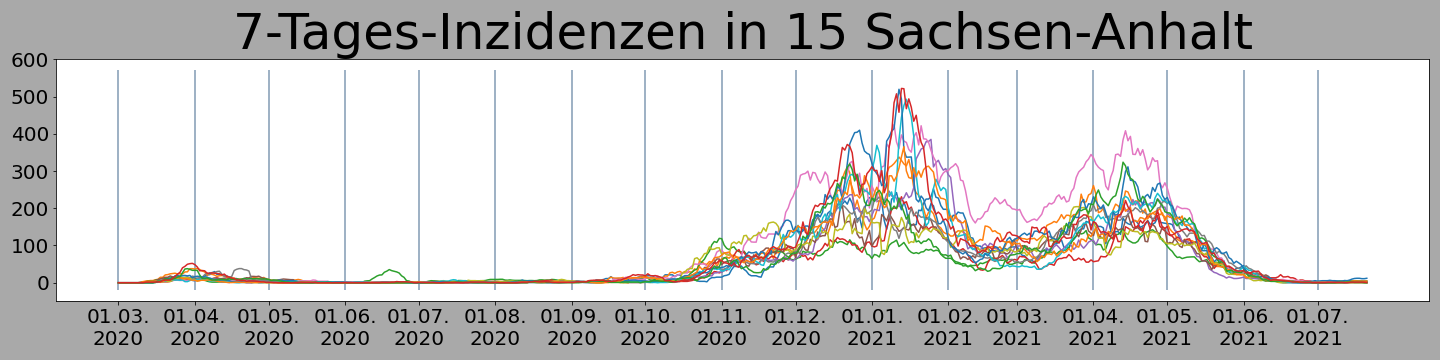
\includegraphics[width=\textwidth]{figures/Anhang/15_Sachsen-Anhalt.png}
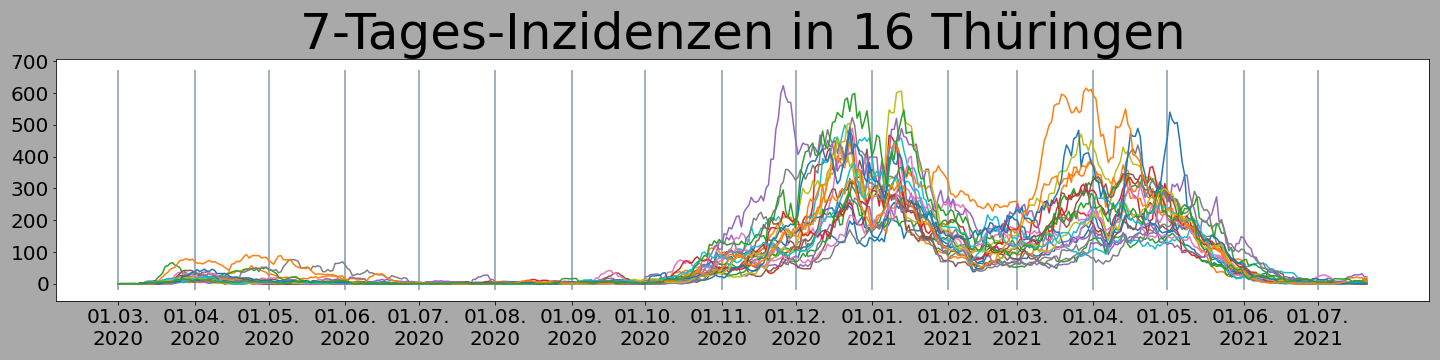
\includegraphics[width=\textwidth]{figures/Anhang/16_Thüringen.png}
\newpage
\section{Die deutschen Landkreise sortiert nach ihrer Bevölkerungsdichte}
\label{tab:counties_by_pop_density}
\begin{enumerate}[itemsep=-6mm]
\item 12070 LK Prignitz (35.60)
\item 15081 LK Altmarkkreis Salzwedel (36.11)
\item 12073 LK Uckermark (38.60)
\item 12068 LK Ostprignitz-Ruppin (39.11)
\item 3354 LK Lüchow-Dannenberg (39.48)
\item 13076 LK Ludwigslust-Parchim (44.43)
\item 15090 LK Stendal (45.62)
\item 13071 LK Mecklenburgische Seenplatte (46.92)
\item 12062 LK Elbe-Elster (53.50)
\item 15086 LK Jerichower Land (56.35)
\item 7232 LK Bitburg-Prüm (60.84)
\item 13075 LK Vorpommern-Greifswald (62.00)
\item 13072 LK Rostock (62.91)
\item 3360 LK Uelzen (63.21)
\item 15091 LK Wittenberg (64.26)
\item 9374 LK Neustadt a.d.Waldnaab (66.10)
\item 9377 LK Tirschenreuth (66.40)
\item 7233 LK Vulkaneifel (66.54)
\item 16069 LK Hildburghausen (67.42)
\item 12071 LK Spree-Neiße (68.45)
\item 16075 LK Saale-Orla-Kreis (69.73)
\item 13073 LK Vorpommern-Rügen (70.97)
\item 16065 LK Kyffhäuserkreis (71.52)
\item 15083 LK Börde (71.91)
\item 6535 LK Vogelsbergkreis (72.50)
\item 13074 LK Nordwestmecklenburg (74.06)
\item 3358 LK Heidekreis (74.80)
\item 12061 LK Dahme-Spreewald (74.91)
\item 9673 LK Rhön-Grabfeld (78.00)
\item 12067 LK Oder-Spree (79.03)
\item 3357 LK Rotenburg (Wümme) (79.04)
\item 9276 LK Regen (79.30)
\item 1054 LK Nordfriesland (79.47)
\item 9272 LK Freyung-Grafenau (79.49)
\item 9575 LK Neustadt a.d.Aisch-Bad Windsheim (79.71)
\item 12072 LK Teltow-Fläming (80.69)
\item 9472 LK Bayreuth (81.39)
\item 9371 LK Amberg-Sulzbach (82.09)
\item 12069 LK Potsdam-Mittelmark (83.45)
\item 9372 LK Cham (83.74)
\item 9278 LK Straubing-Bogen (84.12)
\item 6635 LK Waldeck-Frankenberg (84.71)
\item 16068 LK Sömmerda (86.06)
\item 3462 LK Wittmund (86.26)
\item 3256 LK Nienburg (Weser) (86.70)
\item 9180 LK Garmisch-Partenkirchen (87.40)
\item 9674 LK Haßberge (88.26)
\item 7135 LK Cochem-Zell (88.59)
\item 12066 LK Oberspreewald-Lausitz (89.24)
\item 12064 LK Märkisch-Oderland (90.52)
\item 9672 LK Bad Kissingen (90.80)
\item 16063 LK Wartburgkreis (91.14)
\item 15087 LK Mansfeld-Südharz (92.68)
\item 1051 LK Dithmarschen (93.44)
\item 9571 LK Ansbach (93.62)
\item 12063 LK Havelland (94.29)
\item 9277 LK Rottal-Inn (94.73)
\item 9677 LK Main-Spessart (95.51)
\item 3352 LK Cuxhaven (96.24)
\item 7231 LK Bernkastel-Wittlich (96.28)
\item 14730 LK Nordsachsen (97.44)
\item 9577 LK Weißenburg-Gunzenhausen (97.66)
\item 6636 LK Werra-Meißner-Kreis (98.30)
\item 7340 LK Südwestpfalz (99.44)
\item 16073 LK Saalfeld-Rudolstadt (99.59)
\item 9373 LK Neumarkt i.d.OPf. (100.08)
\item 1059 LK Schleswig-Flensburg (101.12)
\item 15085 LK Harz (101.23)
\item 9376 LK Schwandorf (101.34)
\item 9777 LK Ostallgäu (101.38)
\item 3255 LK Holzminden (101.53)
\item 8128 LK Main-Tauber-Kreis (101.53)
\item 16074 LK Saale-Holzland-Kreis (101.70)
\item 9780 LK Oberallgäu (102.13)
\item 16071 LK Weimarer Land (102.15)
\item 9476 LK Kronach (102.46)
\item 16066 LK Schmalkalden-Meiningen (103.22)
\item 7140 LK Rhein-Hunsrück-Kreis (104.13)
\item 7134 LK Birkenfeld (104.21)
\item 3155 LK Northeim (104.25)
\item 16064 LK Unstrut-Hainich-Kreis (104.46)
\item 9779 LK Donau-Ries (105.04)
\item 9475 LK Hof (106.08)
\item 16061 LK Eichsfeld (106.16)
\item 3461 LK Wesermarsch (107.00)
\item 15082 LK Anhalt-Bitterfeld (108.46)
\item 8437 LK Sigmaringen (108.71)
\item 9477 LK Kulmbach (108.76)
\item 3251 LK Diepholz (109.14)
\item 9176 LK Eichstätt (109.43)
\item 6632 LK Hersfeld-Rotenburg (110.04)
\item 9279 LK Dingolfing-Landau (110.09)
\item 3151 LK Gifhorn (112.55)
\item 3454 LK Emsland (113.43)
\item 16076 LK Greiz (115.05)
\item 9173 LK Bad Tölz-Wolfratshausen (115.06)
\item 9182 LK Miesbach (115.35)
\item 9273 LK Kelheim (115.54)
\item 3351 LK Celle (115.56)
\item 9189 LK Traunstein (115.56)
\item 6634 LK Schwalm-Eder-Kreis (116.79)
\item 16062 LK Nordhausen (116.84)
\item 5762 LK Höxter (116.89)
\item 7333 LK Donnersbergkreis (116.92)
\item 12065 LK Oberhavel (117.63)
\item 9778 LK Unterallgäu (118.24)
\item 9274 LK Landshut (118.60)
\item 1057 LK Plön (118.89)
\item 14626 LK Görlitz (119.33)
\item 9479 LK Wunsiedel i.Fichtelgebirge (119.82)
\item 3453 LK Cloppenburg (120.19)
\item 9773 LK Dillingen a.d.Donau (122.04)
\item 7336 LK Kusel (122.58)
\item 3458 LK Oldenburg (122.98)
\item 14625 LK Bautzen (124.81)
\item 12060 LK Barnim (124.88)
\item 9275 LK Passau (125.70)
\item 9172 LK Berchtesgadener Land (125.97)
\item 16070 LK Ilm-Kreis (126.01)
\item 15084 LK Burgenlandkreis (126.02)
\item 9471 LK Bamberg (126.15)
\item 1058 LK Rendsburg-Eckernförde (126.44)
\item 15088 LK Saalekreis (127.60)
\item 8225 LK Neckar-Odenwald-Kreis (127.72)
\item 9478 LK Lichtenfels (128.50)
\item 1061 LK Steinburg (128.78)
\item 9185 LK Neuburg-Schrobenhausen (131.50)
\item 15089 LK Salzlandkreis (131.77)
\item 5958 LK Hochsauerlandkreis (132.65)
\item 8127 LK Schwäbisch Hall (132.68)
\item 16072 LK Sonneberg (133.32)
\item 9675 LK Kitzingen (133.37)
\item 7235 LK Trier-Saarburg (135.17)
\item 3154 LK Helmstedt (135.17)
\item 8237 LK Freudenstadt (135.84)
\item 9678 LK Schweinfurt (137.29)
\item 9271 LK Deggendorf (138.55)
\item 3355 LK Lüneburg (138.82)
\item 9375 LK Regensburg (139.25)
\item 3456 LK Grafschaft Bentheim (139.72)
\item 9190 LK Weilheim-Schongau (140.07)
\item 3153 LK Goslar (140.74)
\item 9576 LK Roth (141.63)
\item 8426 LK Biberach (142.87)
\item 14522 LK Mittelsachsen (143.64)
\item 9183 LK Mühldorf a.Inn (143.83)
\item 16067 LK Gotha (144.19)
\item 1055 LK Ostholstein (144.71)
\item 8126 LK Hohenlohekreis (145.07)
\item 8425 LK Alb-Donau-Kreis (145.30)
\item 3452 LK Aurich (146.62)
\item 9473 LK Coburg (146.85)
\item 14628 LK Sächsische Schweiz-Osterzgebirge (148.19)
\item 9181 LK Landsberg a.Lech (149.75)
\item 8337 LK Waldshut (151.31)
\item 6437 LK Odenwaldkreis (154.88)
\item 5366 LK Euskirchen (154.93)
\item 14729 LK Leipzig (156.19)
\item 7141 LK Rhein-Lahn-Kreis (156.59)
\item 16077 LK Altenburger Land (156.89)
\item 1053 LK Herzogtum Lauenburg (156.90)
\item 9177 LK Erding (158.61)
\item 3455 LK Friesland (159.86)
\item 14523 LK Vogtlandkreis (159.94)
\item 3457 LK Leer (160.07)
\item 6631 LK Fulda (161.64)
\item 3158 LK Wolfenbüttel (165.26)
\item 7131 LK Ahrweiler (165.35)
\item 7335 LK Kaiserslautern (165.50)
\item 14627 LK Meißen (165.56)
\item 9774 LK Günzburg (166.46)
\item 9679 LK Würzburg (167.94)
\item 9186 LK Pfaffenhofen a.d.Ilm (168.55)
\item 3459 LK Osnabrück (168.94)
\item 3359 LK Stade (169.58)
\item 3451 LK Ammerland (171.21)
\item 9771 LK Aichach-Friedberg (172.72)
\item 7337 LK Südliche Weinstraße (172.92)
\item 3361 LK Verden (173.92)
\item 3356 LK Osterholz (174.55)
\item 8436 LK Ravensburg (175.02)
\item 3460 LK Vechta (175.60)
\item 9676 LK Miltenberg (180.13)
\item 9474 LK Forchheim (180.78)
\item 9187 LK Rosenheim (181.30)
\item 8325 LK Rottweil (181.89)
\item 10046 LK Sankt Wendel (182.70)
\item 6633 LK Kassel (182.92)
\item 14521 LK Erzgebirgskreis (183.13)
\item 7133 LK Bad Kreuznach (183.36)
\item 10042 LK Merzig-Wadern (185.42)
\item 3159 LK Göttingen (185.91)
\item 3252 LK Hameln-Pyrmont (186.33)
\item 5966 LK Olpe (188.36)
\item 8315 LK Breisgau-Hochschwarzwald (191.57)
\item 8327 LK Tuttlingen (191.93)
\item 9171 LK Altötting (195.65)
\item 6534 LK Marburg-Biedenkopf (195.93)
\item 5558 LK Coesfeld (198.41)
\item 8235 LK Calw (199.83)
\item 7132 LK Altenkirchen (201.01)
\item 3353 LK Harburg (203.83)
\item 7143 LK Westerwaldkreis (204.03)
\item 1060 LK Segeberg (206.07)
\item 8417 LK Zollernalbkreis (206.60)
\item 8326 LK Schwarzwald-Baar-Kreis (207.28)
\item 8136 LK Ostalbkreis (208.03)
\item 5570 LK Warendorf (210.84)
\item 8135 LK Heidenheim (211.76)
\item 9574 LK Nürnberger Land (214.11)
\item 7331 LK Alzey-Worms (220.71)
\item 7332 LK Bad Dürkheim (223.52)
\item 9178 LK Freising (225.41)
\item 5974 LK Soest (227.15)
\item 3254 LK Hildesheim (228.55)
\item 6439 LK Rheingau-Taunus-Kreis (230.66)
\item 8317 LK Ortenaukreis (231.89)
\item 6533 LK Limburg-Weilburg (232.80)
\item 3257 LK Schaumburg (233.54)
\item 9772 LK Augsburg (236.64)
\item 6532 LK Lahn-Dill-Kreis (237.96)
\item 9572 LK Erlangen-Höchstadt (243.24)
\item 5970 LK Siegen-Wittgenstein (244.38)
\item 8316 LK Emmendingen (244.71)
\item 5774 LK Paderborn (247.09)
\item 9671 LK Aschaffenburg (249.37)
\item 5566 LK Steinfurt (249.78)
\item 3157 LK Peine (251.49)
\item 5154 LK Kleve (253.32)
\item 9776 LK Lindau (253.85)
\item 9175 LK Ebersberg (261.16)
\item 5554 LK Borken (261.34)
\item 7137 LK Mayen-Koblenz (262.71)
\item 8415 LK Reutlingen (263.02)
\item 9174 LK Dachau (267.29)
\item 5770 LK Minden-Lübbecke (269.65)
\item 7334 LK Germersheim (278.61)
\item 5766 LK Lippe (279.17)
\item 6440 LK Wetteraukreis (280.31)
\item 9188 LK Starnberg (280.75)
\item 5358 LK Düren (281.41)
\item 8336 LK Lörrach (283.52)
\item 7138 LK Neuwied (291.39)
\item 5374 LK Oberbergischer Kreis (296.44)
\item 6435 LK Main-Kinzig-Kreis (301.30)
\item 8216 LK Rastatt (313.54)
\item 8125 LK Heilbronn (313.72)
\item 12051 SK Brandenburg a.d.Havel (314.58)
\item 6531 LK Gießen (316.70)
\item 1062 LK Stormarn (318.89)
\item 15001 SK Dessau-Roßlau (325.08)
\item 8435 LK Bodenseekreis (327.11)
\item 14524 LK Zwickau (331.45)
\item 10045 LK Saarpfalz-Kreis (339.44)
\item 9775 LK Neu-Ulm (339.97)
\item 8236 LK Enzkreis (348.34)
\item 7339 LK Mainz-Bingen (349.30)
\item 8335 LK Konstanz (350.57)
\item 16054 SK Suhl (359.18)
\item 6431 LK Bergstraße (376.28)
\item 5754 LK Gütersloh (376.70)
\item 9573 LK Fürth (383.80)
\item 5962 LK Märkischer Kreis (386.81)
\item 12053 SK Frankfurt (Oder) (389.89)
\item 8211 SK Baden-Baden (394.48)
\item 8117 LK Göppingen (402.00)
\item 16056 SK Eisenach (404.58)
\item 5370 LK Heinsberg (407.38)
\item 8215 LK Karlsruhe (410.76)
\item 9561 SK Ansbach (418.95)
\item 10044 LK Saarlouis (423.45)
\item 8416 LK Tübingen (440.13)
\item 5170 LK Wesel (441.33)
\item 3402 SK Emden (449.07)
\item 6432 LK Darmstadt-Dieburg (453.14)
\item 7316 SK Neustadt a.d.Weinstraße (454.29)
\item 3102 SK Salzgitter (463.65)
\item 7320 SK Zweibrücken (483.04)
\item 6434 LK Hochtaunuskreis (493.09)
\item 1056 LK Pinneberg (496.40)
\item 8119 LK Rems-Murr-Kreis (498.77)
\item 3241 Region Hannover (504.02)
\item 9179 LK Fürstenfeldbruck (504.63)
\item 7338 LK Rhein-Pfalz-Kreis (508.00)
\item 8226 LK Rhein-Neckar-Kreis (517.37)
\item 5382 LK Rhein-Sieg-Kreis (521.57)
\item 9184 LK München (527.71)
\item 10043 LK Neunkirchen (529.77)
\item 5166 LK Viersen (530.26)
\item 5758 LK Herford (556.29)
\item 7313 SK Landau i.d.Pfalz (565.34)
\item 12052 SK Cottbus (602.29)
\item 9363 SK Weiden i.d.OPf. (605.20)
\item 3103 SK Wolfsburg (606.93)
\item 6433 LK Groß-Gerau (608.61)
\item 16052 SK Gera (611.24)
\item 9764 SK Memmingen (631.64)
\item 8115 LK Böblingen (636.92)
\item 5378 LK Rheinisch-Bergischer Kreis (646.79)
\item 7317 SK Pirmasens (654.05)
\item 5362 LK Rhein-Erft-Kreis (669.34)
\item 9263 SK Straubing (705.98)
\item 3405 SK Wilhelmshaven (708.12)
\item 7312 SK Kaiserslautern (713.74)
\item 5978 LK Unna (727.94)
\item 13004 SK Schwerin (735.67)
\item 9262 SK Passau (750.62)
\item 7319 SK Worms (768.65)
\item 16055 SK Weimar (772.60)
\item 5162 LK Rhein-Kreis Neuss (783.40)
\item 9464 SK Hof (786.98)
\item 5954 LK Ennepe-Ruhr-Kreis (789.06)
\item 5334 StädteRegion Aachen (790.54)
\item 5915 SK Hamm (790.88)
\item 16051 SK Erfurt (791.77)
\item 8118 LK Ludwigsburg (794.77)
\item 10041 LK Stadtverband Saarbrücken (798.94)
\item 5562 LK Recklinghausen (806.93)
\item 9361 SK Amberg (836.63)
\item 8116 LK Esslingen (836.83)
\item 9463 SK Coburg (853.31)
\item 12054 SK Potsdam (963.50)
\item 7211 SK Trier (964.92)
\item 16053 SK Jena (969.41)
\item 6438 LK Offenbach (1000.03)
\item 9565 SK Schwabach (1007.16)
\item 1003 SK Lübeck (1022.93)
\item 9161 SK Ingolstadt (1028.17)
\item 5515 SK Münster (1039.25)
\item 8421 SK Ulm (1063.04)
\item 7111 SK Koblenz (1076.89)
\item 6436 LK Main-Taunus-Kreis (1077.20)
\item 9763 SK Kempten (1093.88)
\item 9762 SK Kaufbeuren (1098.03)
\item 9261 SK Landshut (1108.96)
\item 14511 SK Chemnitz (1112.67)
\item 7311 SK Frankenthal (1116.06)
\item 9462 SK Bayreuth (1116.14)
\item 1004 SK Neumünster (1123.16)
\item 9661 SK Aschaffenburg (1146.90)
\item 5512 SK Bottrop (1173.13)
\item 5914 SK Hagen (1177.24)
\item 7318 SK Speyer (1181.35)
\item 15003 SK Magdeburg (1184.71)
\item 5158 LK Mettmann (1190.65)
\item 13003 SK Rostock (1236.48)
\item 3401 SK Delmenhorst (1242.49)
\item 8121 SK Heilbronn (1258.60)
\item 8231 SK Pforzheim (1283.68)
\item 5711 SK Bielefeld (1290.85)
\item 3101 SK Braunschweig (1297.31)
\item 6411 SK Darmstadt (1299.31)
\item 6414 SK Wiesbaden (1367.95)
\item 3404 SK Osnabrück (1375.78)
\item 9461 SK Bamberg (1407.94)
\item 9562 SK Erlangen (1443.07)
\item 9663 SK Würzburg (1458.20)
\item 8221 SK Heidelberg (1478.74)
\item 4012 SK Bremerhaven (1483.07)
\item 8311 SK Freiburg i.Breisgau (1500.23)
\item 5120 SK Remscheid (1503.35)
\item 9662 SK Schweinfurt (1506.19)
\item 5116 SK Mönchengladbach (1528.98)
\item 11009 SK Berlin Treptow-Köpenick (1586.19)
\item 3403 SK Oldenburg (1631.36)
\item 5114 SK Krefeld (1664.19)
\item 14612 SK Dresden (1694.41)
\item 9163 SK Rosenheim (1727.63)
\item 4011 SK Bremen (1743.98)
\item 15002 SK Halle (1758.65)
\item 5122 SK Solingen (1789.94)
\item 8212 SK Karlsruhe (1794.67)
\item 1001 SK Flensburg (1833.24)
\item 5117 SK Mülheim a.d.Ruhr (1870.33)
\item 9362 SK Regensburg (1917.84)
\item 6611 SK Kassel (1936.46)
\item 14713 SK Leipzig (1982.44)
\item 9761 SK Augsburg (2025.77)
\item 9563 SK Fürth (2030.43)
\item 5316 SK Leverkusen (2078.83)
\item 5913 SK Dortmund (2104.24)
\item 5124 SK Wuppertal (2109.81)
\item 5112 SK Duisburg (2140.13)
\item 8222 SK Mannheim (2142.45)
\item 1002 SK Kiel (2198.97)
\item 7314 SK Ludwigshafen (2213.76)
\item 7315 SK Mainz (2238.90)
\item 5314 SK Bonn (2328.50)
\item 5513 SK Gelsenkirchen (2466.57)
\item 2000 SK Hamburg (2489.29)
\item 5911 SK Bochum (2525.55)
\item 11005 SK Berlin Spandau (2571.74)
\item 5315 SK Köln (2675.86)
\item 5119 SK Oberhausen (2720.89)
\item 9564 SK Nürnberg (2762.59)
\item 5113 SK Essen (2769.50)
\item 5111 SK Düsseldorf (2861.04)
\item 6413 SK Offenbach (2875.04)
\item 11012 SK Berlin Reinickendorf (2903.61)
\item 11006 SK Berlin Steglitz-Zehlendorf (2942.69)
\item 8111 SK Stuttgart (3033.65)
\item 5916 SK Herne (3039.06)
\item 6412 SK Frankfurt am Main (3077.83)
\item 11003 SK Berlin Pankow (3850.86)
\item 11010 SK Berlin Marzahn-Hellersdorf (4247.24)
\item 9162 SK München (4765.75)
\item 11004 SK Berlin Charlottenburg-Wilmersdorf (5162.54)
\item 11011 SK Berlin Lichtenberg (5489.14)
\item 11007 SK Berlin Tempelhof-Schöneberg (6433.60)
\item 11008 SK Berlin Neukölln (7136.56)
\item 11001 SK Berlin Mitte (9511.23)
\item 11002 SK Berlin Friedrichshain-Kreuzberg (13807.03)
\end{enumerate}
\section{Die deutschen Landkreise lexikographisch sortiert nach ihren Gemeindeschlüsseln}
\label{tab:counties_by_admunitid}
\begin{tabular}{c c}
    1001&SK Flensburg\\ 
    1002&SK Kiel\\ 
    1003&SK Lübeck\\ 
    1004&SK Neumünster\\ 
    10041&LK Stadtverband Saarbrücken\\ 
    10042&LK Merzig-Wadern\\ 
    10043&LK Neunkirchen\\ 
    10044&LK Saarlouis\\ 
    10045&LK Saarpfalz-Kreis\\ 
    10046&LK Sankt Wendel\\ 
    1051&LK Dithmarschen\\ 
    1053&LK Herzogtum Lauenburg\\ 
    1054&LK Nordfriesland\\ 
    1055&LK Ostholstein\\ 
    1056&LK Pinneberg\\ 
    1057&LK Plön\\ 
    1058&LK Rendsburg-Eckernförde\\ 
    1059&LK Schleswig-Flensburg\\ 
    1060&LK Segeberg\\ 
    1061&LK Steinburg\\ 
    1062&LK Stormarn\\ 
    11001&SK Berlin Mitte\\ 
    11002&SK Berlin Friedrichshain-Kreuzberg\\ 
    11003&SK Berlin Pankow\\ 
    11004&SK Berlin Charlottenburg-Wilmersdorf\\ 
    11005&SK Berlin Spandau\\ 
    11006&SK Berlin Steglitz-Zehlendorf\\ 
    11007&SK Berlin Tempelhof-Schöneberg\\ 
    11008&SK Berlin Neukölln\\ 
    11009&SK Berlin Treptow-Köpenick\\ 
    11010&SK Berlin Marzahn-Hellersdorf\\ 
    11011&SK Berlin Lichtenberg\\ 
    11012&SK Berlin Reinickendorf\\ 
    12051&SK Brandenburg a.d.Havel\\ 
    12052&SK Cottbus\\ 
    12053&SK Frankfurt (Oder)\\ 
    12054&SK Potsdam\\ 
    12060&LK Barnim\\ 
    12061&LK Dahme-Spreewald\\ 
    12062&LK Elbe-Elster\\ 
    12063&LK Havelland\\ 
    12064&LK Märkisch-Oderland\\ 
    12065&LK Oberhavel\\ 
    12066&LK Oberspreewald-Lausitz\\ 
    12067&LK Oder-Spree\\ 
    12068&LK Ostprignitz-Ruppin\\ 
    12069&LK Potsdam-Mittelmark\\ 
    12070&LK Prignitz\\ 
    12071&LK Spree-Neiße\\ 
    12072&LK Teltow-Fläming\\ 
    12073&LK Uckermark\\ 
    13003&SK Rostock\\ 
    13004&SK Schwerin\\ 
    13071&LK Mecklenburgische Seenplatte\\ 
    13072&LK Rostock\\ 
    13073&LK Vorpommern-Rügen\\ 
    13074&LK Nordwestmecklenburg\\ 
    13075&LK Vorpommern-Greifswald\\ 
    13076&LK Ludwigslust-Parchim\\ 
    14511&SK Chemnitz\\ 
    14521&LK Erzgebirgskreis\\ 
    14522&LK Mittelsachsen\\ 
    14523&LK Vogtlandkreis\\ 
    14524&LK Zwickau\\ 
    14612&SK Dresden\\ 
    14625&LK Bautzen\\ 
    14626&LK Görlitz\\ 
    14627&LK Meißen\\ 
    14628&LK Sächsische Schweiz-Osterzgebirge\\ 
    14713&SK Leipzig\\ 
    14729&LK Leipzig\\ 
    14730&LK Nordsachsen\\ 
    15001&SK Dessau-Roßlau\\ 
    15002&SK Halle\\ 
    15003&SK Magdeburg\\ 
    15081&LK Altmarkkreis Salzwedel\\ 
    15082&LK Anhalt-Bitterfeld\\ 
    15083&LK Börde\\ 
    15084&LK Burgenlandkreis\\ 
    15085&LK Harz\\ 
    15086&LK Jerichower Land\\ 
    15087&LK Mansfeld-Südharz\\ 
    15088&LK Saalekreis\\ 
    15089&LK Salzlandkreis\\ 
    15090&LK Stendal\\ 
    15091&LK Wittenberg\\ 
    16051&SK Erfurt\\ 
    16052&SK Gera\\ 
    16053&SK Jena\\ 
    16054&SK Suhl\\ 
    16055&SK Weimar\\ 
    16056&SK Eisenach\\ 
    16061&LK Eichsfeld\\ 
    16062&LK Nordhausen\\ 
    16063&LK Wartburgkreis\\ 
    16064&LK Unstrut-Hainich-Kreis\\ 
    16065&LK Kyffhäuserkreis\\ 
    16066&LK Schmalkalden-Meiningen\\ 
    16067&LK Gotha\\ 
    16068&LK Sömmerda\\ 
    16069&LK Hildburghausen\\ 
    16070&LK Ilm-Kreis\\ 
    16071&LK Weimarer Land\\ 
    16072&LK Sonneberg\\ 
    16073&LK Saalfeld-Rudolstadt\\ 
    16074&LK Saale-Holzland-Kreis\\ 
    16075&LK Saale-Orla-Kreis\\ 
    16076&LK Greiz\\ 
    16077&LK Altenburger Land\\ 
    2000&SK Hamburg\\ 
    3101&SK Braunschweig\\ 
    3102&SK Salzgitter\\ 
    3103&SK Wolfsburg\\ 
    3151&LK Gifhorn\\ 
    3153&LK Goslar\\ 
    3154&LK Helmstedt\\ 
    3155&LK Northeim\\ 
    3157&LK Peine\\ 
    3158&LK Wolfenbüttel\\ 
    3159&LK Göttingen\\ 
    3241&Region Hannover\\ 
    3251&LK Diepholz\\ 
    3252&LK Hameln-Pyrmont\\ 
    3254&LK Hildesheim\\ 
    3255&LK Holzminden\\ 
    3256&LK Nienburg (Weser)\\ 
    3257&LK Schaumburg\\ 
    3351&LK Celle\\ 
    3352&LK Cuxhaven\\ 
    3353&LK Harburg\\ 
    3354&LK Lüchow-Dannenberg\\ 
    3355&LK Lüneburg\\ 
    3356&LK Osterholz\\ 
    3357&LK Rotenburg (Wümme)\\ 
    3358&LK Heidekreis\\ 
    3359&LK Stade\\ 
    3360&LK Uelzen\\ 
    3361&LK Verden\\ 
    3401&SK Delmenhorst\\ 
    3402&SK Emden\\ 
    3403&SK Oldenburg\\ 
    3404&SK Osnabrück\\ 
    3405&SK Wilhelmshaven\\ 
    3451&LK Ammerland\\ 
    3452&LK Aurich\\ 
    3453&LK Cloppenburg\\ 
    3454&LK Emsland\\ 
    3455&LK Friesland\\ 
    3456&LK Grafschaft Bentheim\\ 
    3457&LK Leer\\ 
    3458&LK Oldenburg\\ 
    3459&LK Osnabrück\\ 
    3460&LK Vechta\\ 
    3461&LK Wesermarsch\\ 
    3462&LK Wittmund\\ 
    4011&SK Bremen\\ 
    4012&SK Bremerhaven\\ 
    5111&SK Düsseldorf\\ 
    5112&SK Duisburg\\ 
    5113&SK Essen\\ 
    5114&SK Krefeld\\ 
    5116&SK Mönchengladbach\\ 
    5117&SK Mülheim a.d.Ruhr\\ 
    5119&SK Oberhausen\\ 
    5120&SK Remscheid\\ 
    5122&SK Solingen\\ 
    5124&SK Wuppertal\\ 
    5154&LK Kleve\\ 
    5158&LK Mettmann\\ 
    5162&LK Rhein-Kreis Neuss\\ 
    5166&LK Viersen\\ 
    5170&LK Wesel\\ 
    5314&SK Bonn\\ 
    5315&SK Köln\\ 
    5316&SK Leverkusen\\ 
    5334&StädteRegion Aachen\\ 
    5358&LK Düren\\ 
    5362&LK Rhein-Erft-Kreis\\ 
    5366&LK Euskirchen\\ 
    5370&LK Heinsberg\\ 
    5374&LK Oberbergischer Kreis\\ 
    5378&LK Rheinisch-Bergischer Kreis\\ 
    5382&LK Rhein-Sieg-Kreis\\ 
    5512&SK Bottrop\\ 
    5513&SK Gelsenkirchen\\ 
    5515&SK Münster\\ 
    5554&LK Borken\\ 
    5558&LK Coesfeld\\ 
    5562&LK Recklinghausen\\ 
    5566&LK Steinfurt\\ 
    5570&LK Warendorf\\ 
    5711&SK Bielefeld\\ 
    5754&LK Gütersloh\\ 
    5758&LK Herford\\ 
    5762&LK Höxter\\ 
    5766&LK Lippe\\ 
    5770&LK Minden-Lübbecke\\ 
    5774&LK Paderborn\\ 
    5911&SK Bochum\\ 
    5913&SK Dortmund\\ 
    5914&SK Hagen\\ 
    5915&SK Hamm\\ 
    5916&SK Herne\\ 
    5954&LK Ennepe-Ruhr-Kreis\\ 
    5958&LK Hochsauerlandkreis\\ 
    5962&LK Märkischer Kreis\\ 
    5966&LK Olpe\\ 
    5970&LK Siegen-Wittgenstein\\ 
    5974&LK Soest\\ 
    5978&LK Unna\\ 
    6411&SK Darmstadt\\ 
    6412&SK Frankfurt am Main\\ 
    6413&SK Offenbach\\ 
    6414&SK Wiesbaden\\ 
    6431&LK Bergstraße\\ 
    6432&LK Darmstadt-Dieburg\\ 
    6433&LK Groß-Gerau\\ 
    6434&LK Hochtaunuskreis\\ 
    6435&LK Main-Kinzig-Kreis\\ 
    6436&LK Main-Taunus-Kreis\\ 
    6437&LK Odenwaldkreis\\ 
    6438&LK Offenbach\\ 
    6439&LK Rheingau-Taunus-Kreis\\ 
    6440&LK Wetteraukreis\\ 
    6531&LK Gießen\\ 
    6532&LK Lahn-Dill-Kreis\\ 
    6533&LK Limburg-Weilburg\\ 
    6534&LK Marburg-Biedenkopf\\ 
    6535&LK Vogelsbergkreis\\ 
    6611&SK Kassel\\ 
    6631&LK Fulda\\ 
    6632&LK Hersfeld-Rotenburg\\ 
    6633&LK Kassel\\ 
    6634&LK Schwalm-Eder-Kreis\\ 
    6635&LK Waldeck-Frankenberg\\ 
    6636&LK Werra-Meißner-Kreis\\ 
    7111&SK Koblenz\\ 
    7131&LK Ahrweiler\\ 
    7132&LK Altenkirchen\\ 
    7133&LK Bad Kreuznach\\ 
    7134&LK Birkenfeld\\ 
    7135&LK Cochem-Zell\\ 
    7137&LK Mayen-Koblenz\\ 
    7138&LK Neuwied\\ 
    7140&LK Rhein-Hunsrück-Kreis\\ 
    7141&LK Rhein-Lahn-Kreis\\ 
    7143&LK Westerwaldkreis\\ 
    7211&SK Trier\\ 
    7231&LK Bernkastel-Wittlich\\ 
    7232&LK Bitburg-Prüm\\ 
    7233&LK Vulkaneifel\\ 
    7235&LK Trier-Saarburg\\ 
    7311&SK Frankenthal\\ 
    7312&SK Kaiserslautern\\ 
    7313&SK Landau i.d.Pfalz\\ 
    7314&SK Ludwigshafen\\ 
    7315&SK Mainz\\ 
    7316&SK Neustadt a.d.Weinstraße\\ 
    7317&SK Pirmasens\\ 
    7318&SK Speyer\\ 
    7319&SK Worms\\ 
    7320&SK Zweibrücken\\ 
    7331&LK Alzey-Worms\\ 
    7332&LK Bad Dürkheim\\ 
    7333&LK Donnersbergkreis\\ 
    7334&LK Germersheim\\ 
    7335&LK Kaiserslautern\\ 
    7336&LK Kusel\\ 
    7337&LK Südliche Weinstraße\\ 
    7338&LK Rhein-Pfalz-Kreis\\ 
    7339&LK Mainz-Bingen\\ 
    7340&LK Südwestpfalz\\ 
    8111&SK Stuttgart\\ 
    8115&LK Böblingen\\ 
    8116&LK Esslingen\\ 
    8117&LK Göppingen\\ 
    8118&LK Ludwigsburg\\ 
    8119&LK Rems-Murr-Kreis\\ 
    8121&SK Heilbronn\\ 
    8125&LK Heilbronn\\ 
    8126&LK Hohenlohekreis\\ 
    8127&LK Schwäbisch Hall\\ 
    8128&LK Main-Tauber-Kreis\\ 
    8135&LK Heidenheim\\ 
    8136&LK Ostalbkreis\\ 
    8211&SK Baden-Baden\\ 
    8212&SK Karlsruhe\\ 
    8215&LK Karlsruhe\\ 
    8216&LK Rastatt\\ 
    8221&SK Heidelberg\\ 
    8222&SK Mannheim\\ 
    8225&LK Neckar-Odenwald-Kreis\\ 
    8226&LK Rhein-Neckar-Kreis\\ 
    8231&SK Pforzheim\\ 
    8235&LK Calw\\ 
    8236&LK Enzkreis\\ 
    8237&LK Freudenstadt\\ 
    8311&SK Freiburg i.Breisgau\\ 
    8315&LK Breisgau-Hochschwarzwald\\ 
    8316&LK Emmendingen\\ 
    8317&LK Ortenaukreis\\ 
    8325&LK Rottweil\\ 
    8326&LK Schwarzwald-Baar-Kreis\\ 
    8327&LK Tuttlingen\\ 
    8335&LK Konstanz\\ 
    8336&LK Lörrach\\ 
    8337&LK Waldshut\\ 
    8415&LK Reutlingen\\ 
    8416&LK Tübingen\\ 
    8417&LK Zollernalbkreis\\ 
    8421&SK Ulm\\ 
    8425&LK Alb-Donau-Kreis\\ 
    8426&LK Biberach\\ 
    8435&LK Bodenseekreis\\ 
    8436&LK Ravensburg\\ 
    8437&LK Sigmaringen\\ 
    9161&SK Ingolstadt\\ 
    9162&SK München\\ 
    9163&SK Rosenheim\\ 
    9171&LK Altötting\\ 
    9172&LK Berchtesgadener Land\\ 
    9173&LK Bad Tölz-Wolfratshausen\\ 
    9174&LK Dachau\\ 
    9175&LK Ebersberg\\ 
    9176&LK Eichstätt\\ 
    9177&LK Erding\\ 
    9178&LK Freising\\ 
    9179&LK Fürstenfeldbruck\\ 
    9180&LK Garmisch-Partenkirchen\\ 
    9181&LK Landsberg a.Lech\\ 
    9182&LK Miesbach\\ 
    9183&LK Mühldorf a.Inn\\ 
    9184&LK München\\ 
    9185&LK Neuburg-Schrobenhausen\\ 
    9186&LK Pfaffenhofen a.d.Ilm\\ 
    9187&LK Rosenheim\\ 
    9188&LK Starnberg\\ 
    9189&LK Traunstein\\ 
    9190&LK Weilheim-Schongau\\ 
    9261&SK Landshut\\ 
    9262&SK Passau\\ 
    9263&SK Straubing\\ 
    9271&LK Deggendorf\\ 
    9272&LK Freyung-Grafenau\\ 
    9273&LK Kelheim\\ 
    9274&LK Landshut\\ 
    9275&LK Passau\\ 
    9276&LK Regen\\ 
    9277&LK Rottal-Inn\\ 
    9278&LK Straubing-Bogen\\ 
    9279&LK Dingolfing-Landau\\ 
    9361&SK Amberg\\ 
    9362&SK Regensburg\\ 
    9363&SK Weiden i.d.OPf.\\ 
    9371&LK Amberg-Sulzbach\\ 
    9372&LK Cham\\ 
    9373&LK Neumarkt i.d.OPf.\\ 
    9374&LK Neustadt a.d.Waldnaab\\ 
    9375&LK Regensburg\\ 
    9376&LK Schwandorf\\ 
    9377&LK Tirschenreuth\\ 
    9461&SK Bamberg\\ 
    9462&SK Bayreuth\\ 
    9463&SK Coburg\\ 
    9464&SK Hof\\ 
    9471&LK Bamberg\\ 
    9472&LK Bayreuth\\ 
    9473&LK Coburg\\ 
    9474&LK Forchheim\\ 
    9475&LK Hof\\ 
    9476&LK Kronach\\ 
    9477&LK Kulmbach\\ 
    9478&LK Lichtenfels\\ 
    9479&LK Wunsiedel i.Fichtelgebirge\\ 
    9561&SK Ansbach\\ 
    9562&SK Erlangen\\ 
    9563&SK Fürth\\ 
    9564&SK Nürnberg\\ 
    9565&SK Schwabach\\ 
    9571&LK Ansbach\\ 
    9572&LK Erlangen-Höchstadt\\ 
    9573&LK Fürth\\ 
    9574&LK Nürnberger Land\\ 
    9575&LK Neustadt a.d.Aisch-Bad Windsheim\\ 
    9576&LK Roth\\ 
    9577&LK Weißenburg-Gunzenhausen\\ 
    9661&SK Aschaffenburg\\ 
    9662&SK Schweinfurt\\ 
    9663&SK Würzburg\\ 
    9671&LK Aschaffenburg\\ 
    9672&LK Bad Kissingen\\ 
    9673&LK Rhön-Grabfeld\\ 
    9674&LK Haßberge\\ 
    9675&LK Kitzingen\\ 
    9676&LK Miltenberg\\ 
    9677&LK Main-Spessart\\ 
    9678&LK Schweinfurt\\ 
    9679&LK Würzburg\\ 
    9761&SK Augsburg\\ 
    9762&SK Kaufbeuren\\ 
    9763&SK Kempten\\ 
    9764&SK Memmingen\\ 
    9771&LK Aichach-Friedberg\\ 
    9772&LK Augsburg\\ 
    9773&LK Dillingen a.d.Donau\\ 
    9774&LK Günzburg\\ 
    9775&LK Neu-Ulm\\ 
    9776&LK Lindau\\ 
    9777&LK Ostallgäu\\ 
    9778&LK Unterallgäu\\ 
    9779&LK Donau-Ries\\ 
    9780&LK Oberallgäu\\ 

\end{tabular}
\section{Die Regierungsbezirke sortiert nach ihrer Bevölkerungsdichte}
\label{tab:districts_by_pop_density}
13  Mecklenburg-Vorpommern

12  Brandenburg

15  Sachsen-Anhalt

72  Trier

33  L�neburg

93  Oberpfalz

92  Niederbayern

16  Th�ringen

66  Kassel

94  Oberfranken

96  Unterfranken

34  Weser-Ems

71  Koblenz

1  Schleswig-Holstein

97  Schwaben

65  Gie�en

31  Braunschweig

146  Dresden

84  T�bingen

145  Chemnitz

32  Hannover

83  Freiburg

95  Mittelfranken

147  Leipzig

91  Oberbayern

73  Rheinhessen-Pfalz

57  Detmold

55  M�nster

10  Saarland

81  Stuttgart

82  Karlsruhe

59  Arnsberg

64  Darmstadt

53  K�ln

51  D�sseldorf

4  Bremen

2  Hamburg

11  Berlin


\section{Die Regierungsbezirke lexikographisch sortiert nach den ersten beiden Teilen der Gemeindeschlüssel ihrer Landkreise}
\label{tab:districts_by_admunitid}
1  Schleswig-Holstein

10  Saarland

11  Berlin

12  Brandenburg

13  Mecklenburg-Vorpommern

145  Chemnitz

146  Dresden

147  Leipzig

15  Sachsen-Anhalt

16  Thüringen

2  Hamburg

31  Braunschweig

32  Hannover

33  Lüneburg

34  Weser-Ems

4  Bremen

51  Düsseldorf

53  Köln

55  Münster

57  Detmold

59  Arnsberg

64  Darmstadt

65  Gießen

66  Kassel

71  Koblenz

72  Trier

73  Rheinhessen-Pfalz

81  Stuttgart

82  Karlsruhe

83  Freiburg

84  Tübingen

91  Oberbayern

92  Niederbayern

93  Oberpfalz

94  Oberfranken

95  Mittelfranken

96  Unterfranken

97  Schwaben


\newpage


    % If you want a list of your ToDos at the end of the document
    % don't forget to remove before submission!
    % place it somewhere in the document
\chapter*{ToDo Counters}
\newcounter{ct}%
To Dos: \arabic{todos}; \hspace{1em}%
\setcounter{ct}{0}%
\whiledo {\value{ct} < \value{todos}}%
{%
	\stepcounter {ct}%
    \ref{todo \thect}%
	\ifnum\value{ct} = \value{todos}{}\else{, }\fi
}

Parts to extend: \arabic{extends}; \hspace{1em}%
\setcounter{ct}{0}%
\whiledo {\value{ct} < \value{extends}}%
{%
	\stepcounter {ct}%
	\ref{extend \thect}%
	\ifnum\value{ct} = \value{extends}{}\else{, }\fi
}

Draft parts: \arabic{drafts}; \hspace{1em}%
\setcounter{ct}{0}%
\whiledo {\value{ct} < \value{drafts}}%
{%
	\stepcounter {ct}%
	\ref{draft \thect}%
	\ifnum\value{ct} = \value{drafts}{}\else{, }\fi
}

    
    \printbibliography 
    % bibliography is not in the table of contents per default, add it manually
    % enable the \renewcommand for german header
    \renewcommand{\bibname}{Literaturverzeichnis}
    \addcontentsline{toc}{chapter}{Literaturverzeichnis}
    \newpage
    \thispagestyle{empty}
    \mbox{}
\end{document}
